\begin{appendix} 
\newpage
\section{TMC4671}\label{Appendix:TMC4671}

\subsection{Standard-Schaltkreis TMC4671}

\begin{figure}[h!]
	\centering
	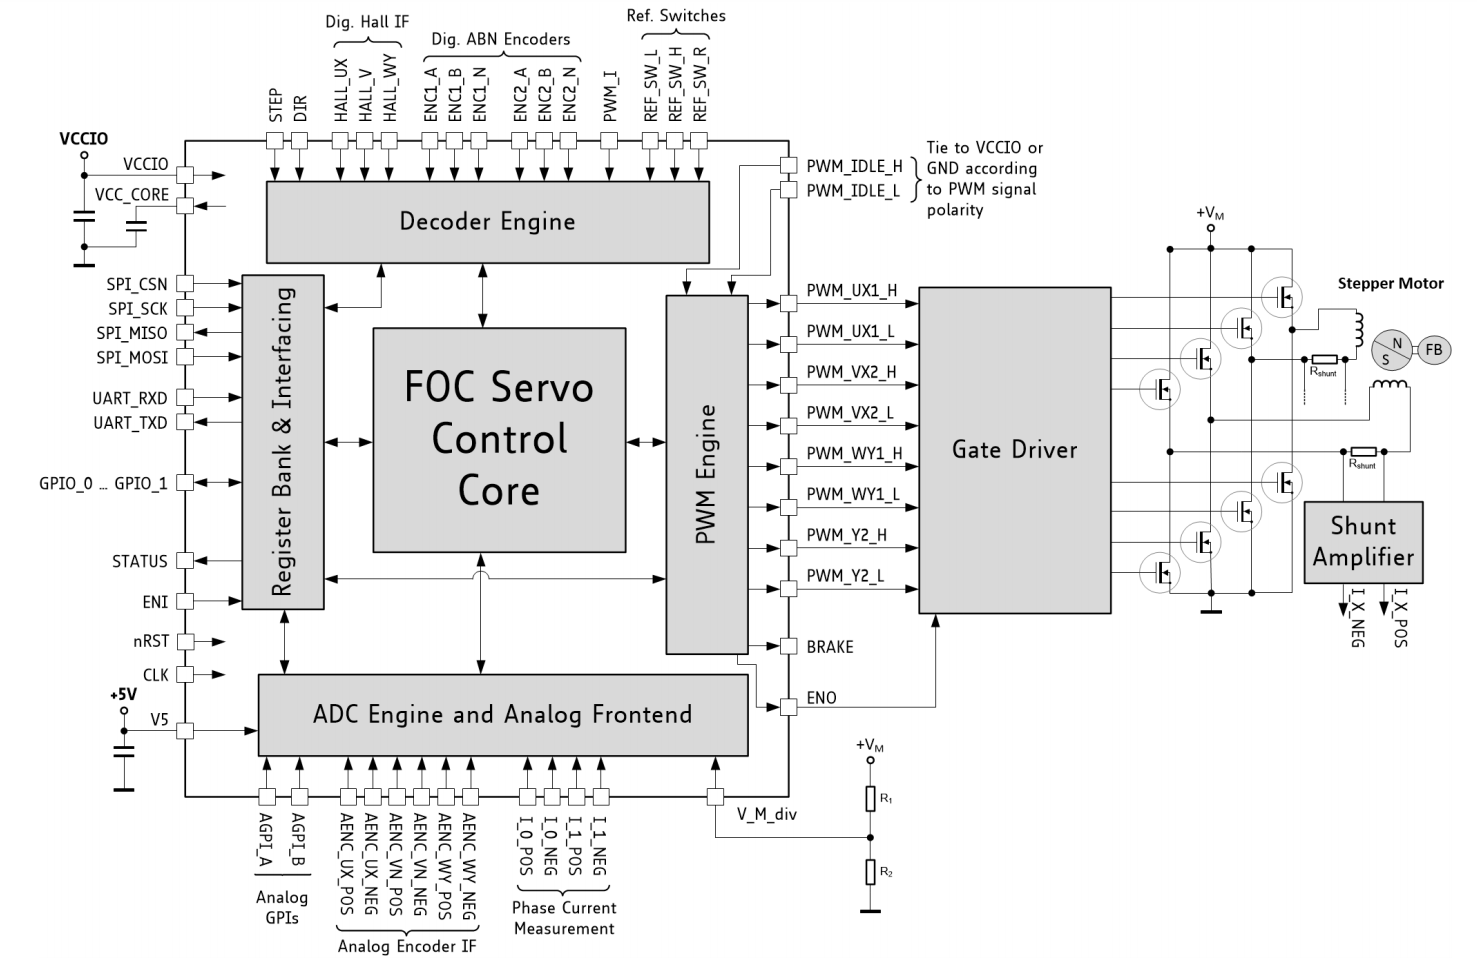
\includegraphics[width=0.8\textwidth]{graphics/Standard_Application_Cirquit_TMC4671}
	\caption{Standard-Anwendungs-Schaltung.}
	\label{fig:Schaltung_TMC4671}
\end{figure}
\todo{cite{TMC4671 Datenblatt}}

\subsection{Blockdiagramm TMC4671}

\begin{figure}[h!]
	\centering
	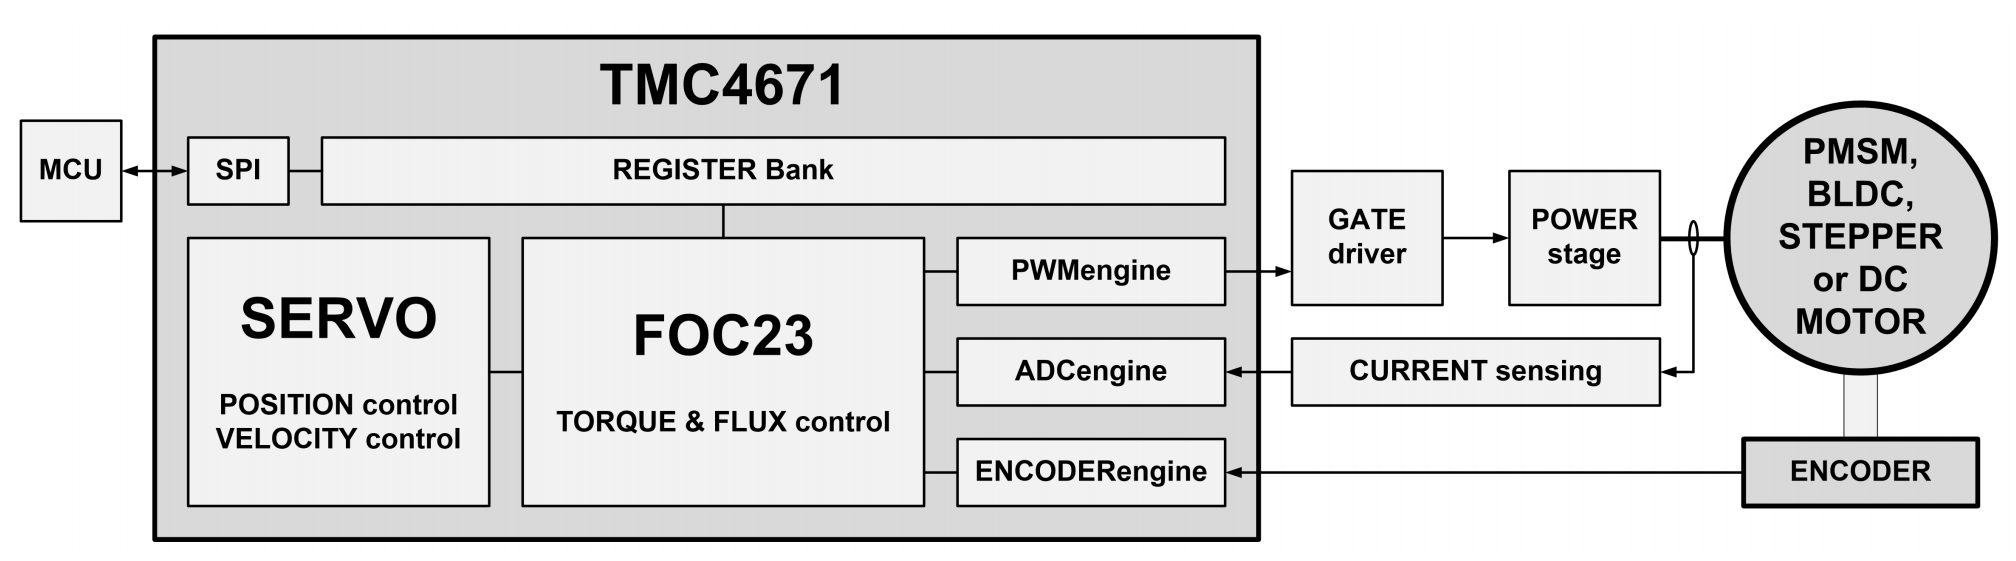
\includegraphics[width=0.8\textwidth]{graphics/Blockdiagramm_TMC4671}
	\caption{Blockdiagramm TMC4671.}
	\label{fig:Blockdiagramm_TMC4671}
\end{figure}

\todo{cite{TMC4671 Datenblatt}}

\newpage

\subsection{Inbetriebnahme TMC4671}

\subsubsection{Setup}\label{Appendix:TMC4671_Setup}

\begin{figure}[h!]
	\centering
	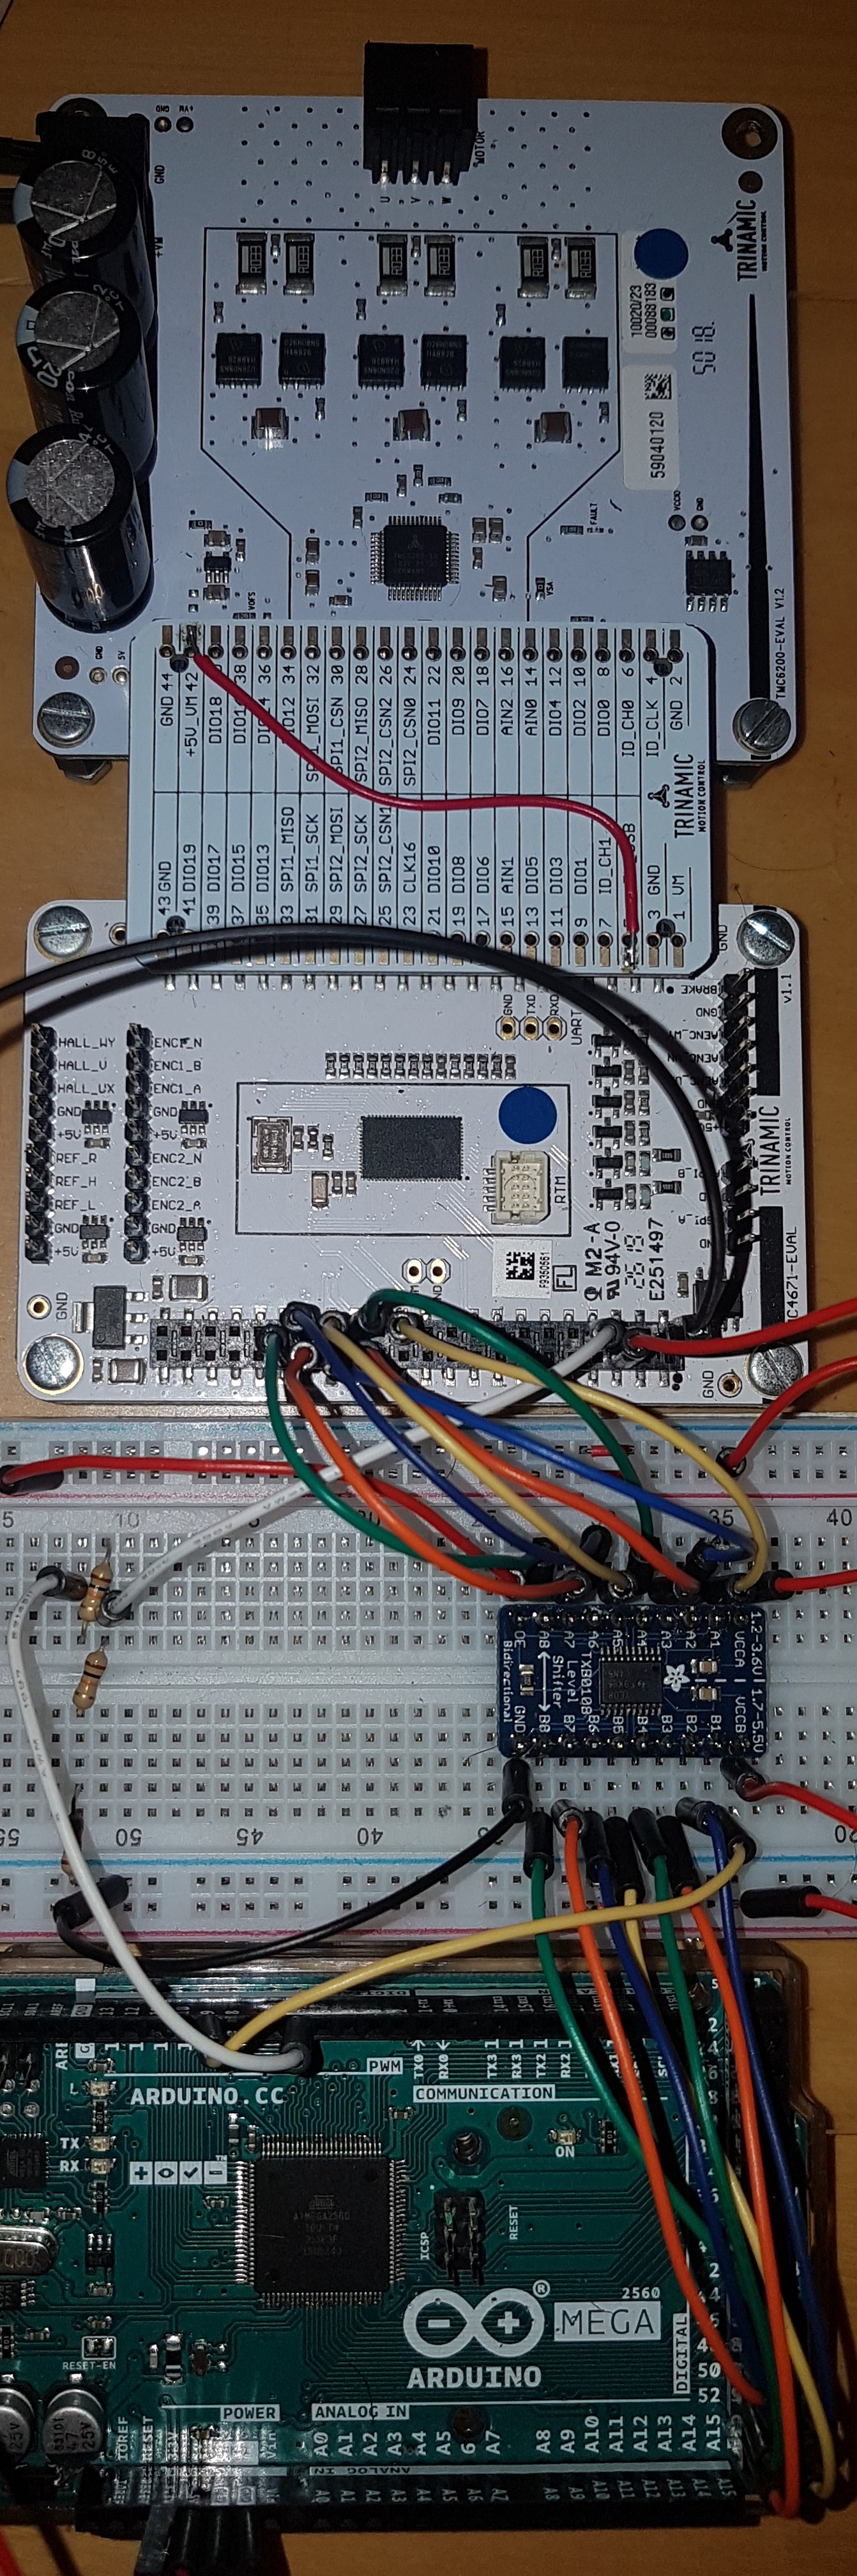
\includegraphics[angle=270,width=\textwidth]{graphics/2_komplett1}
	\caption{Gesamtansicht Setup.}
	\label{fig:2_komplett1}
\end{figure}

\begin{figure}[h!]
	\centering
	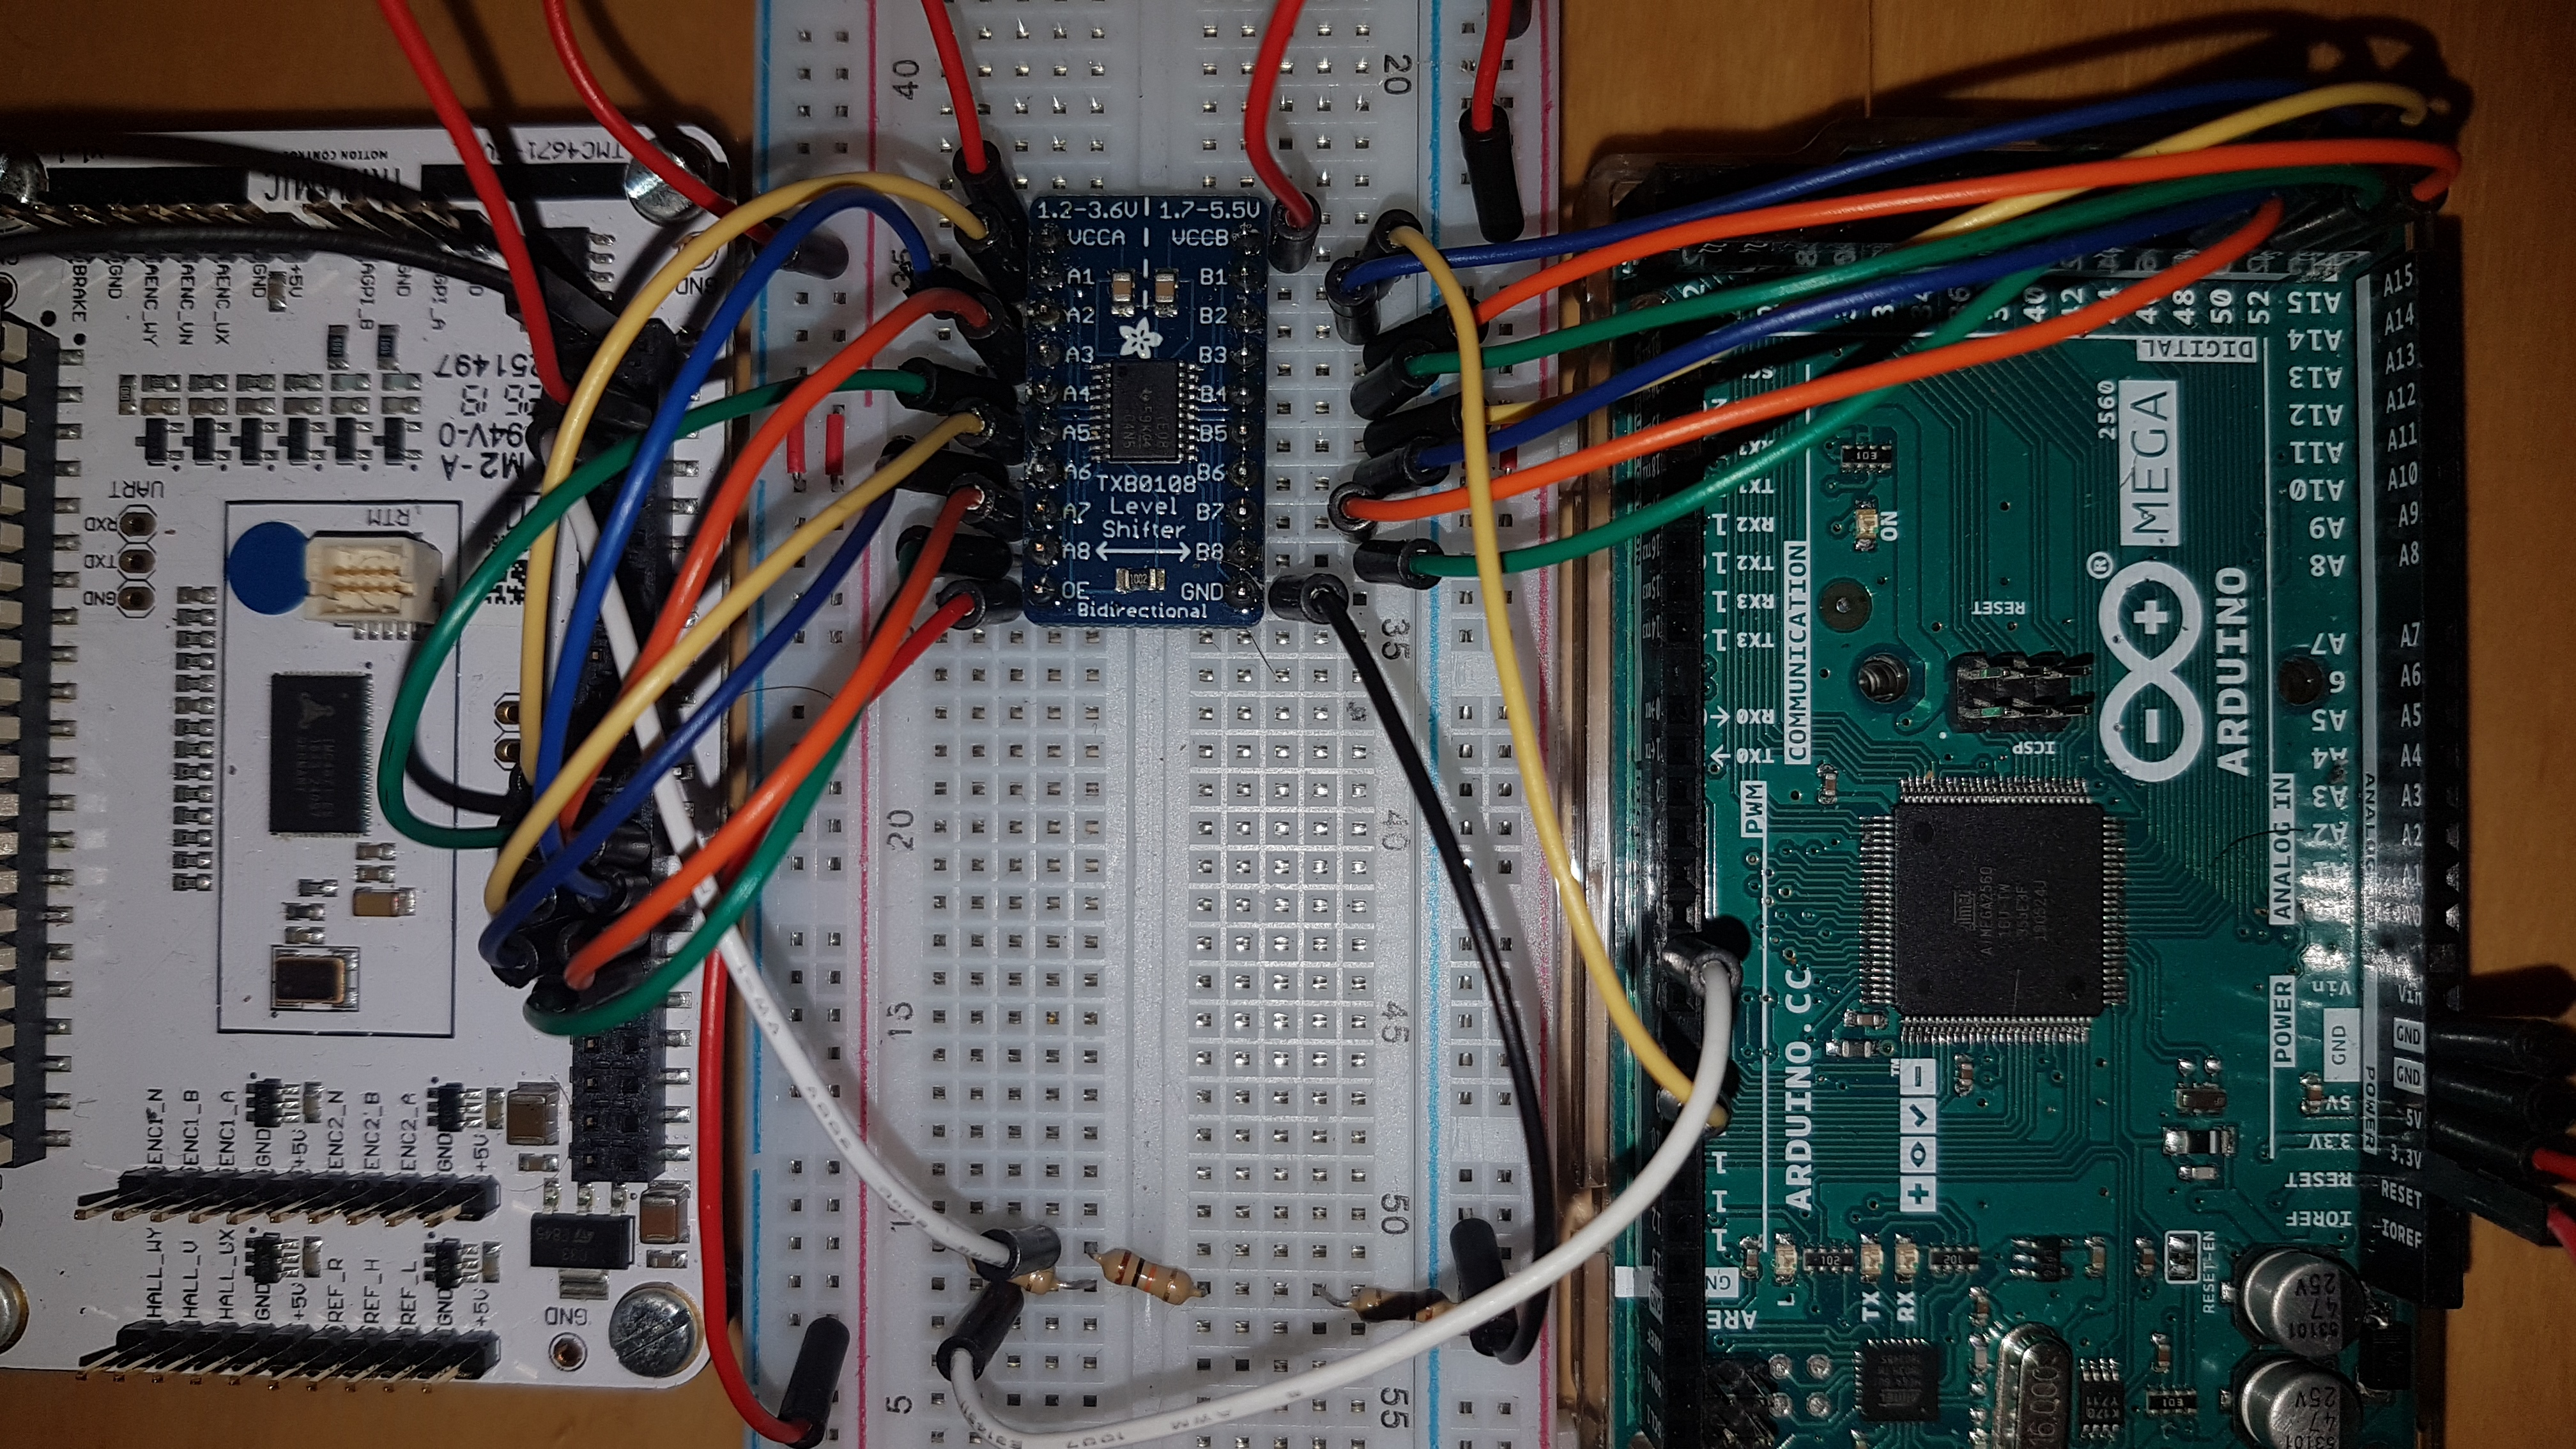
\includegraphics[angle=180,width=\textwidth]{graphics/2_komplett2}
	\caption{Gesamtansicht Setup Wiring.}
	\label{fig:1_komplett}
\end{figure}

\newpage

\begin{figure}[h!]
	\centering
	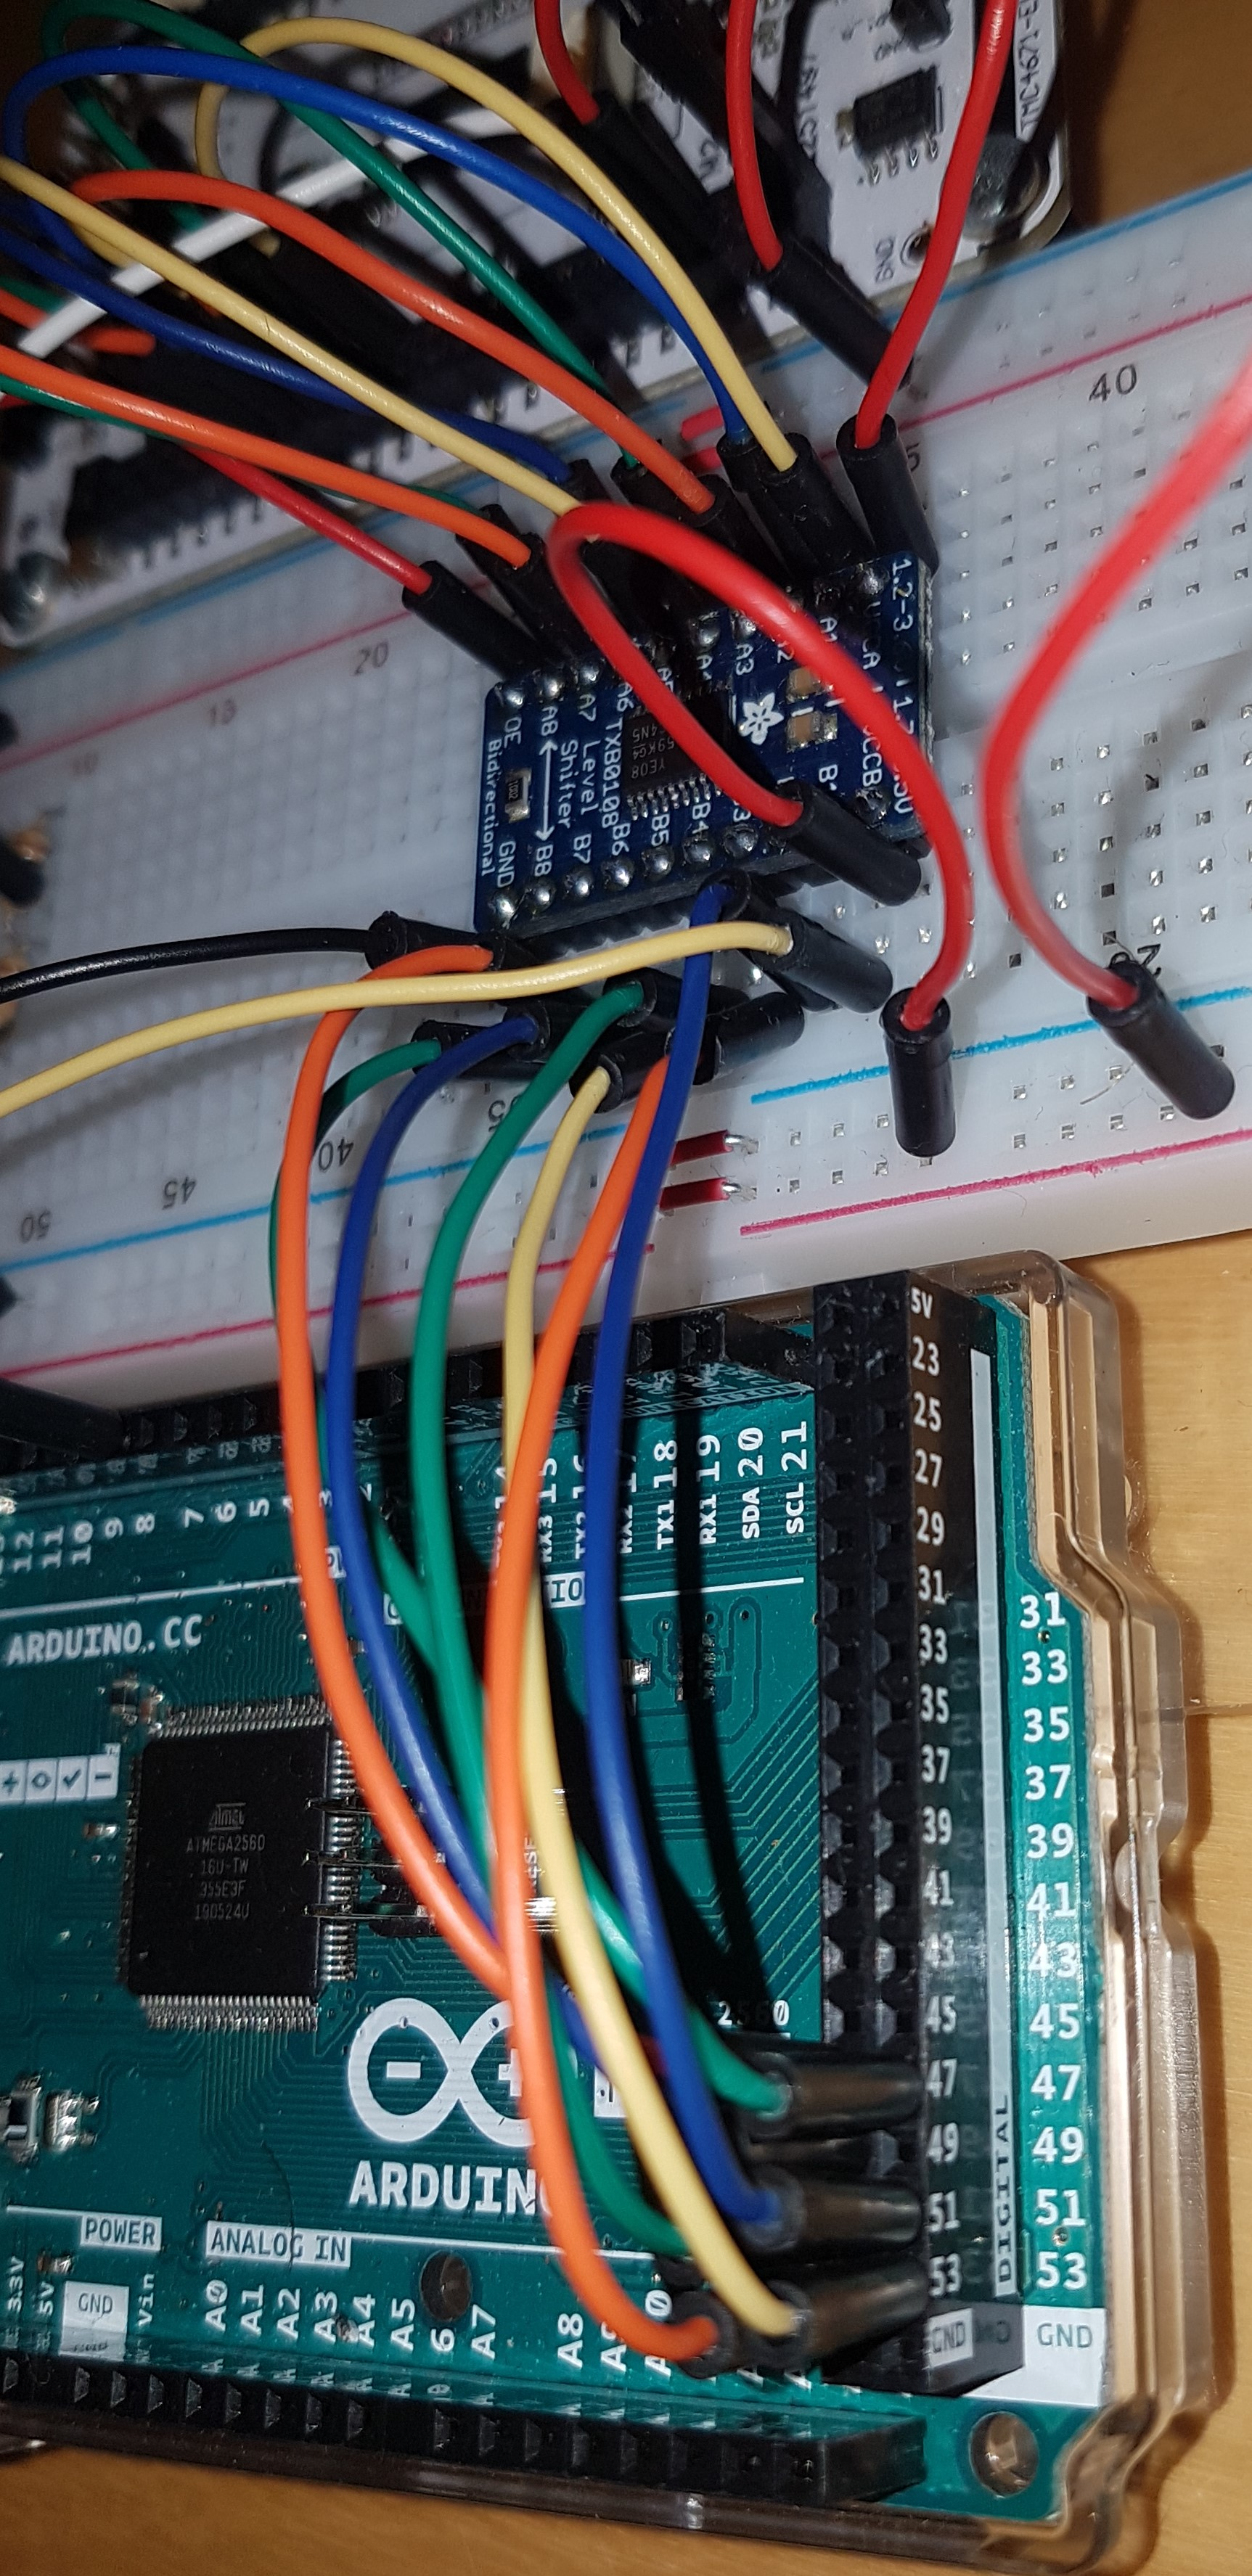
\includegraphics[angle = 270,width=\textwidth]{graphics/2_Arduino}
	\caption{Setup mit Fokus auf Arduino.}
	\label{fig:2_Arduino}
\end{figure}

\begin{figure}[h!]
	\centering
	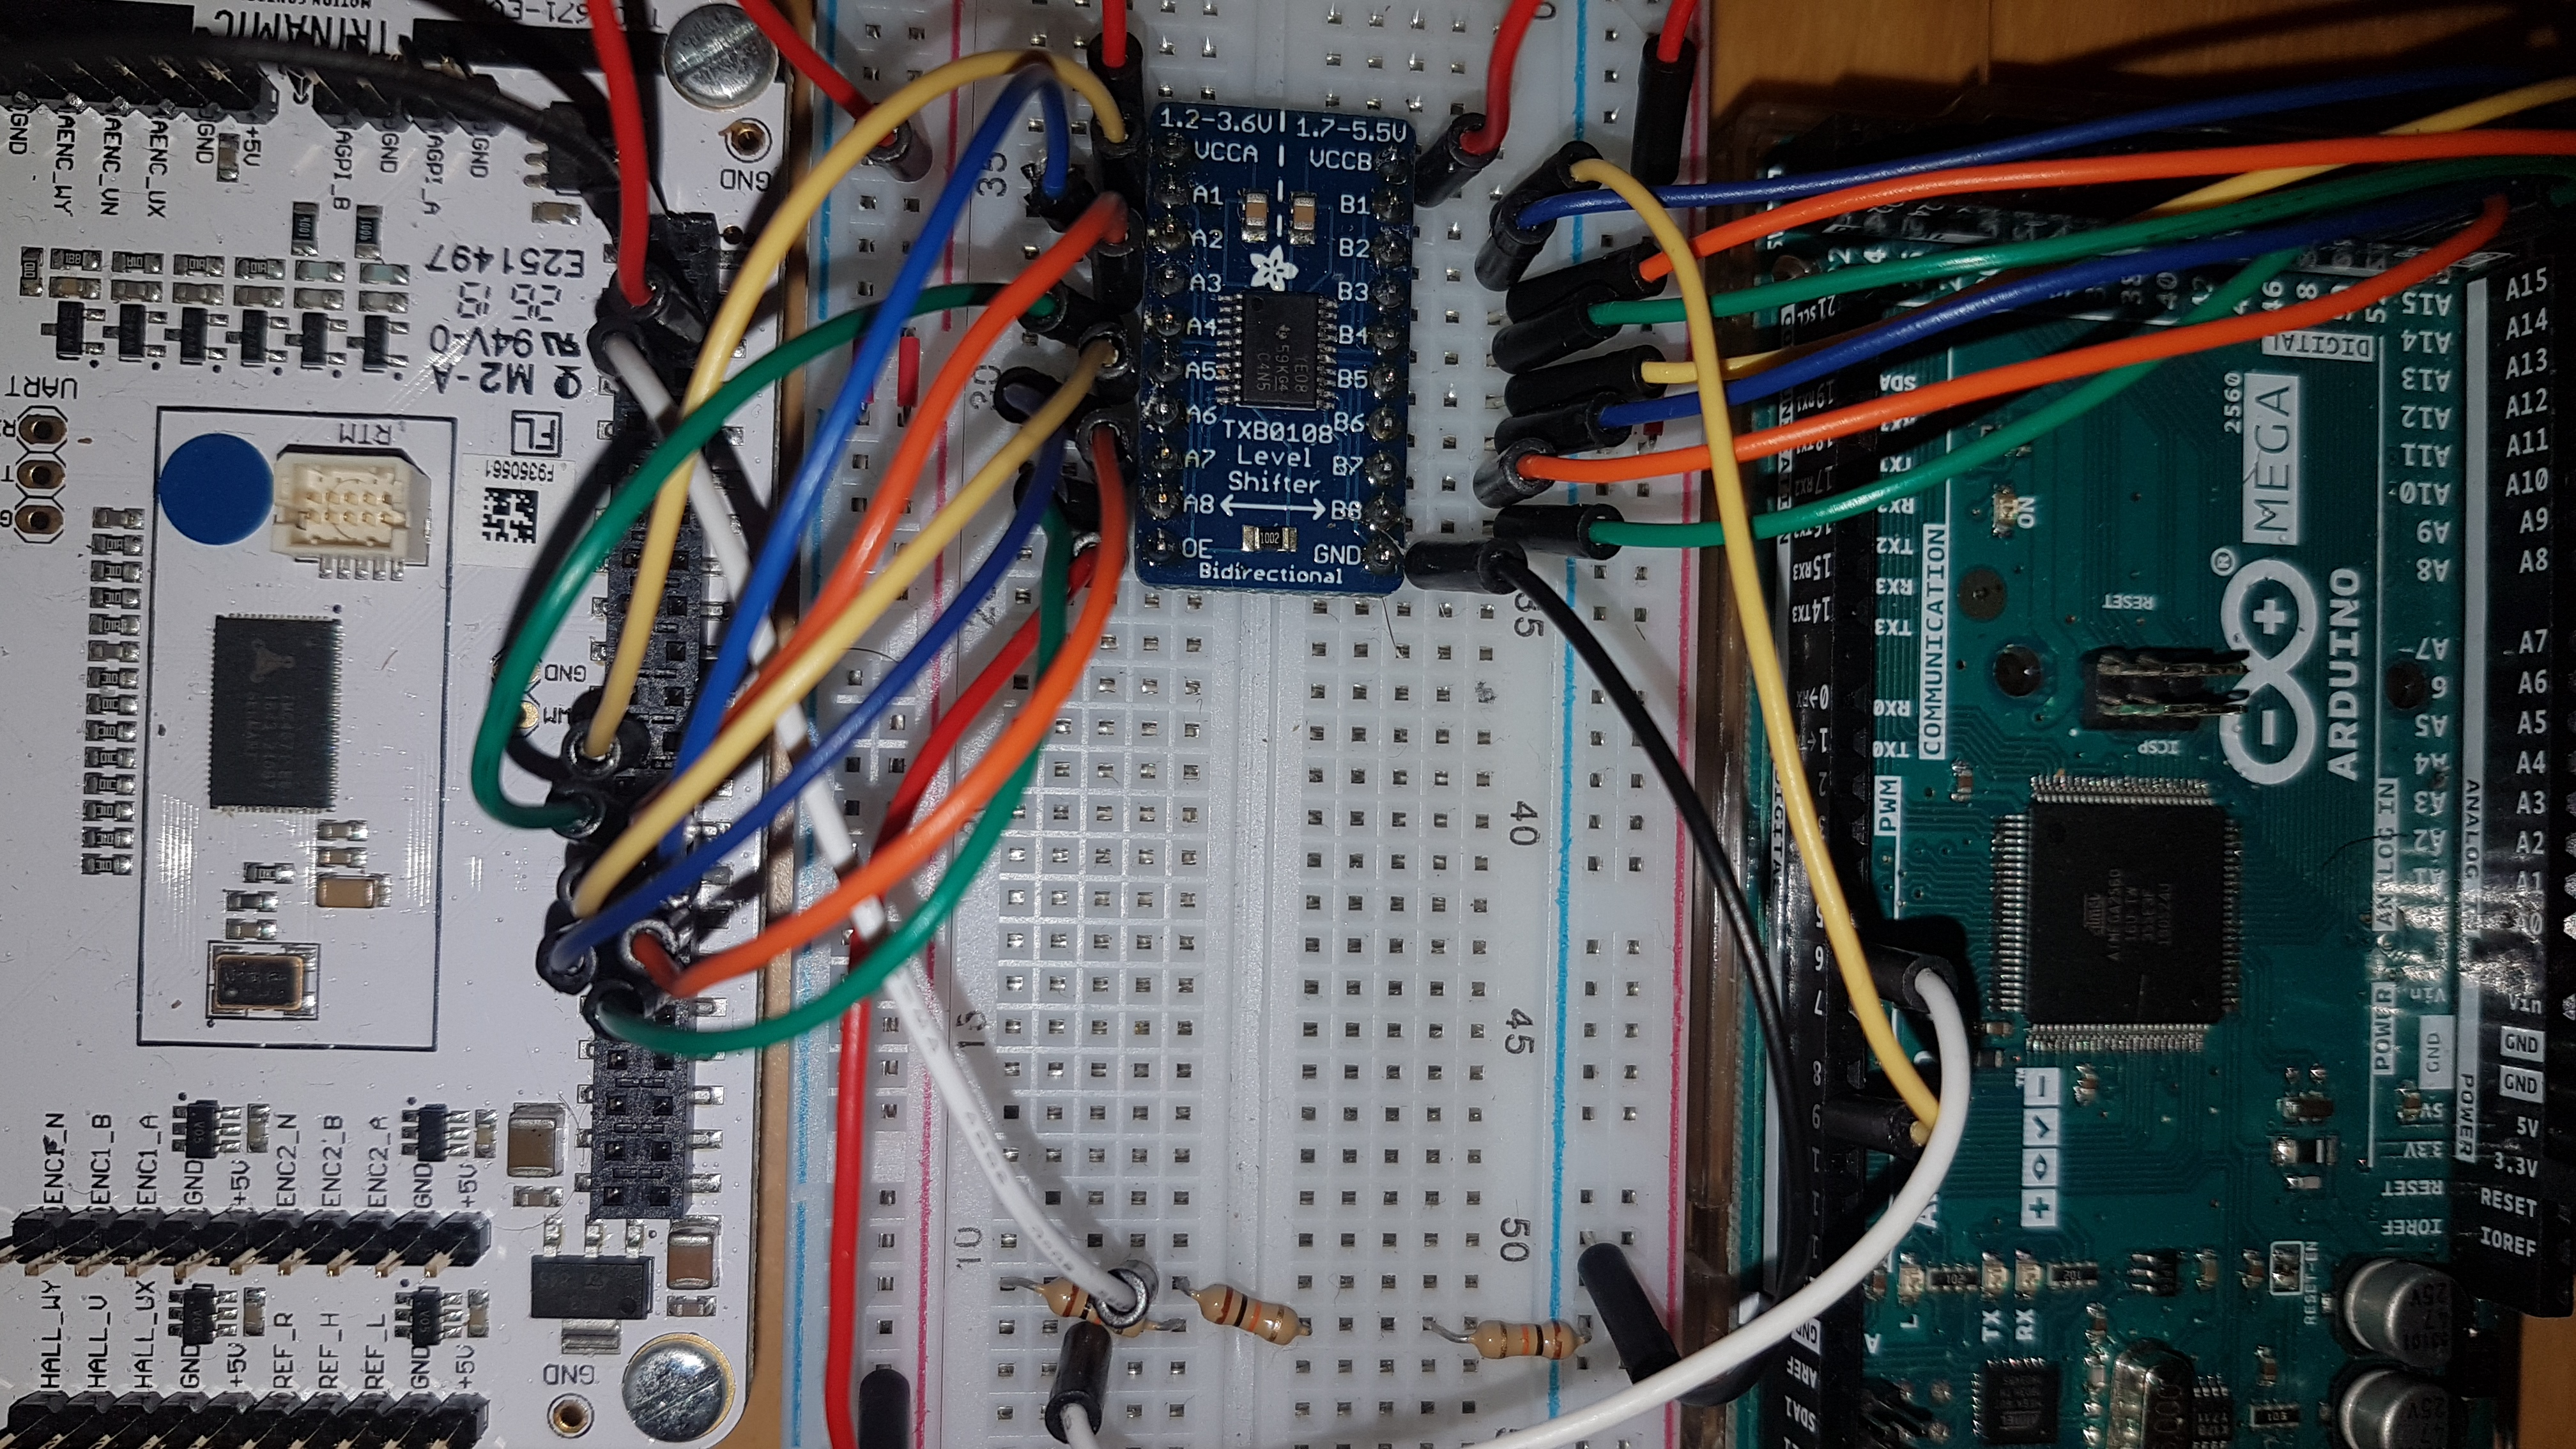
\includegraphics[angle = 180,width=\textwidth]{graphics/2_EVAL}
	\caption{Setup mit Fokus auf TMC4674-EVAL.}
	\label{fig:2_EVAL}
\end{figure}

\newpage

\subsubsection{Inbetriebnahme SPI-Kommunikation}\label{Appendix:TMC4671_SPI}

\begin{figure}[h!]
\center
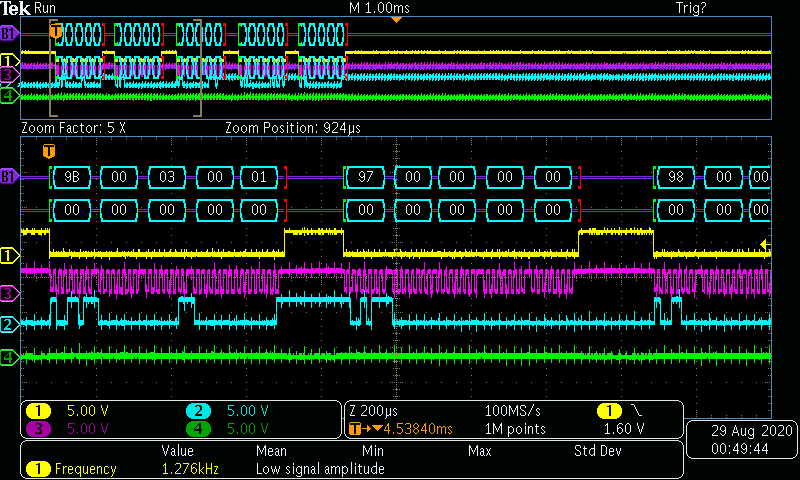
\includegraphics[width = \textwidth]{graphics/TMC4671_Beschreiben_1}
\caption{SPI-Übertragung Write (Hier Motor Pole Pairs).}
\label{fig:TMC4671_Lesen_1}
\end{figure}

\begin{figure}[h!]
\center
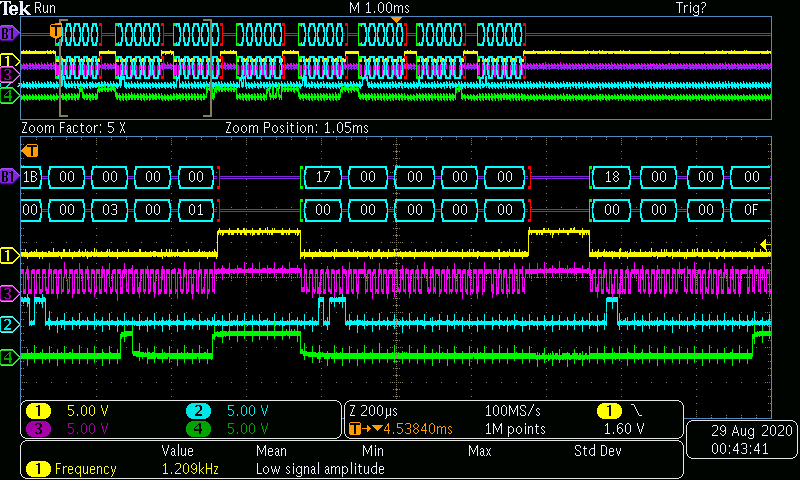
\includegraphics[width = \textwidth]{graphics/TMC4671_Lesen_1}
\caption{SPI-Übertragung Read (Hier Motor Pole Pairs).}
\label{fig:TMC4671_Lesen_1}
\end{figure}

\newpage
\begin{figure}[h!]
\center
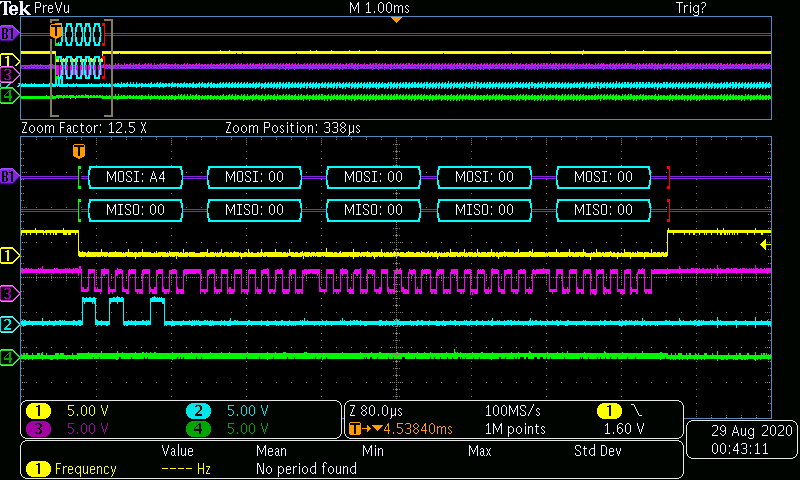
\includegraphics[width = \textwidth]{graphics/TMC4671_TestDrive4}
\caption{Übertragung mit Zoom (Testdrive).}
\label{fig:TMC4671_TestDrive4}
\end{figure}

\newpage

\begin{figure}[h!]
\center
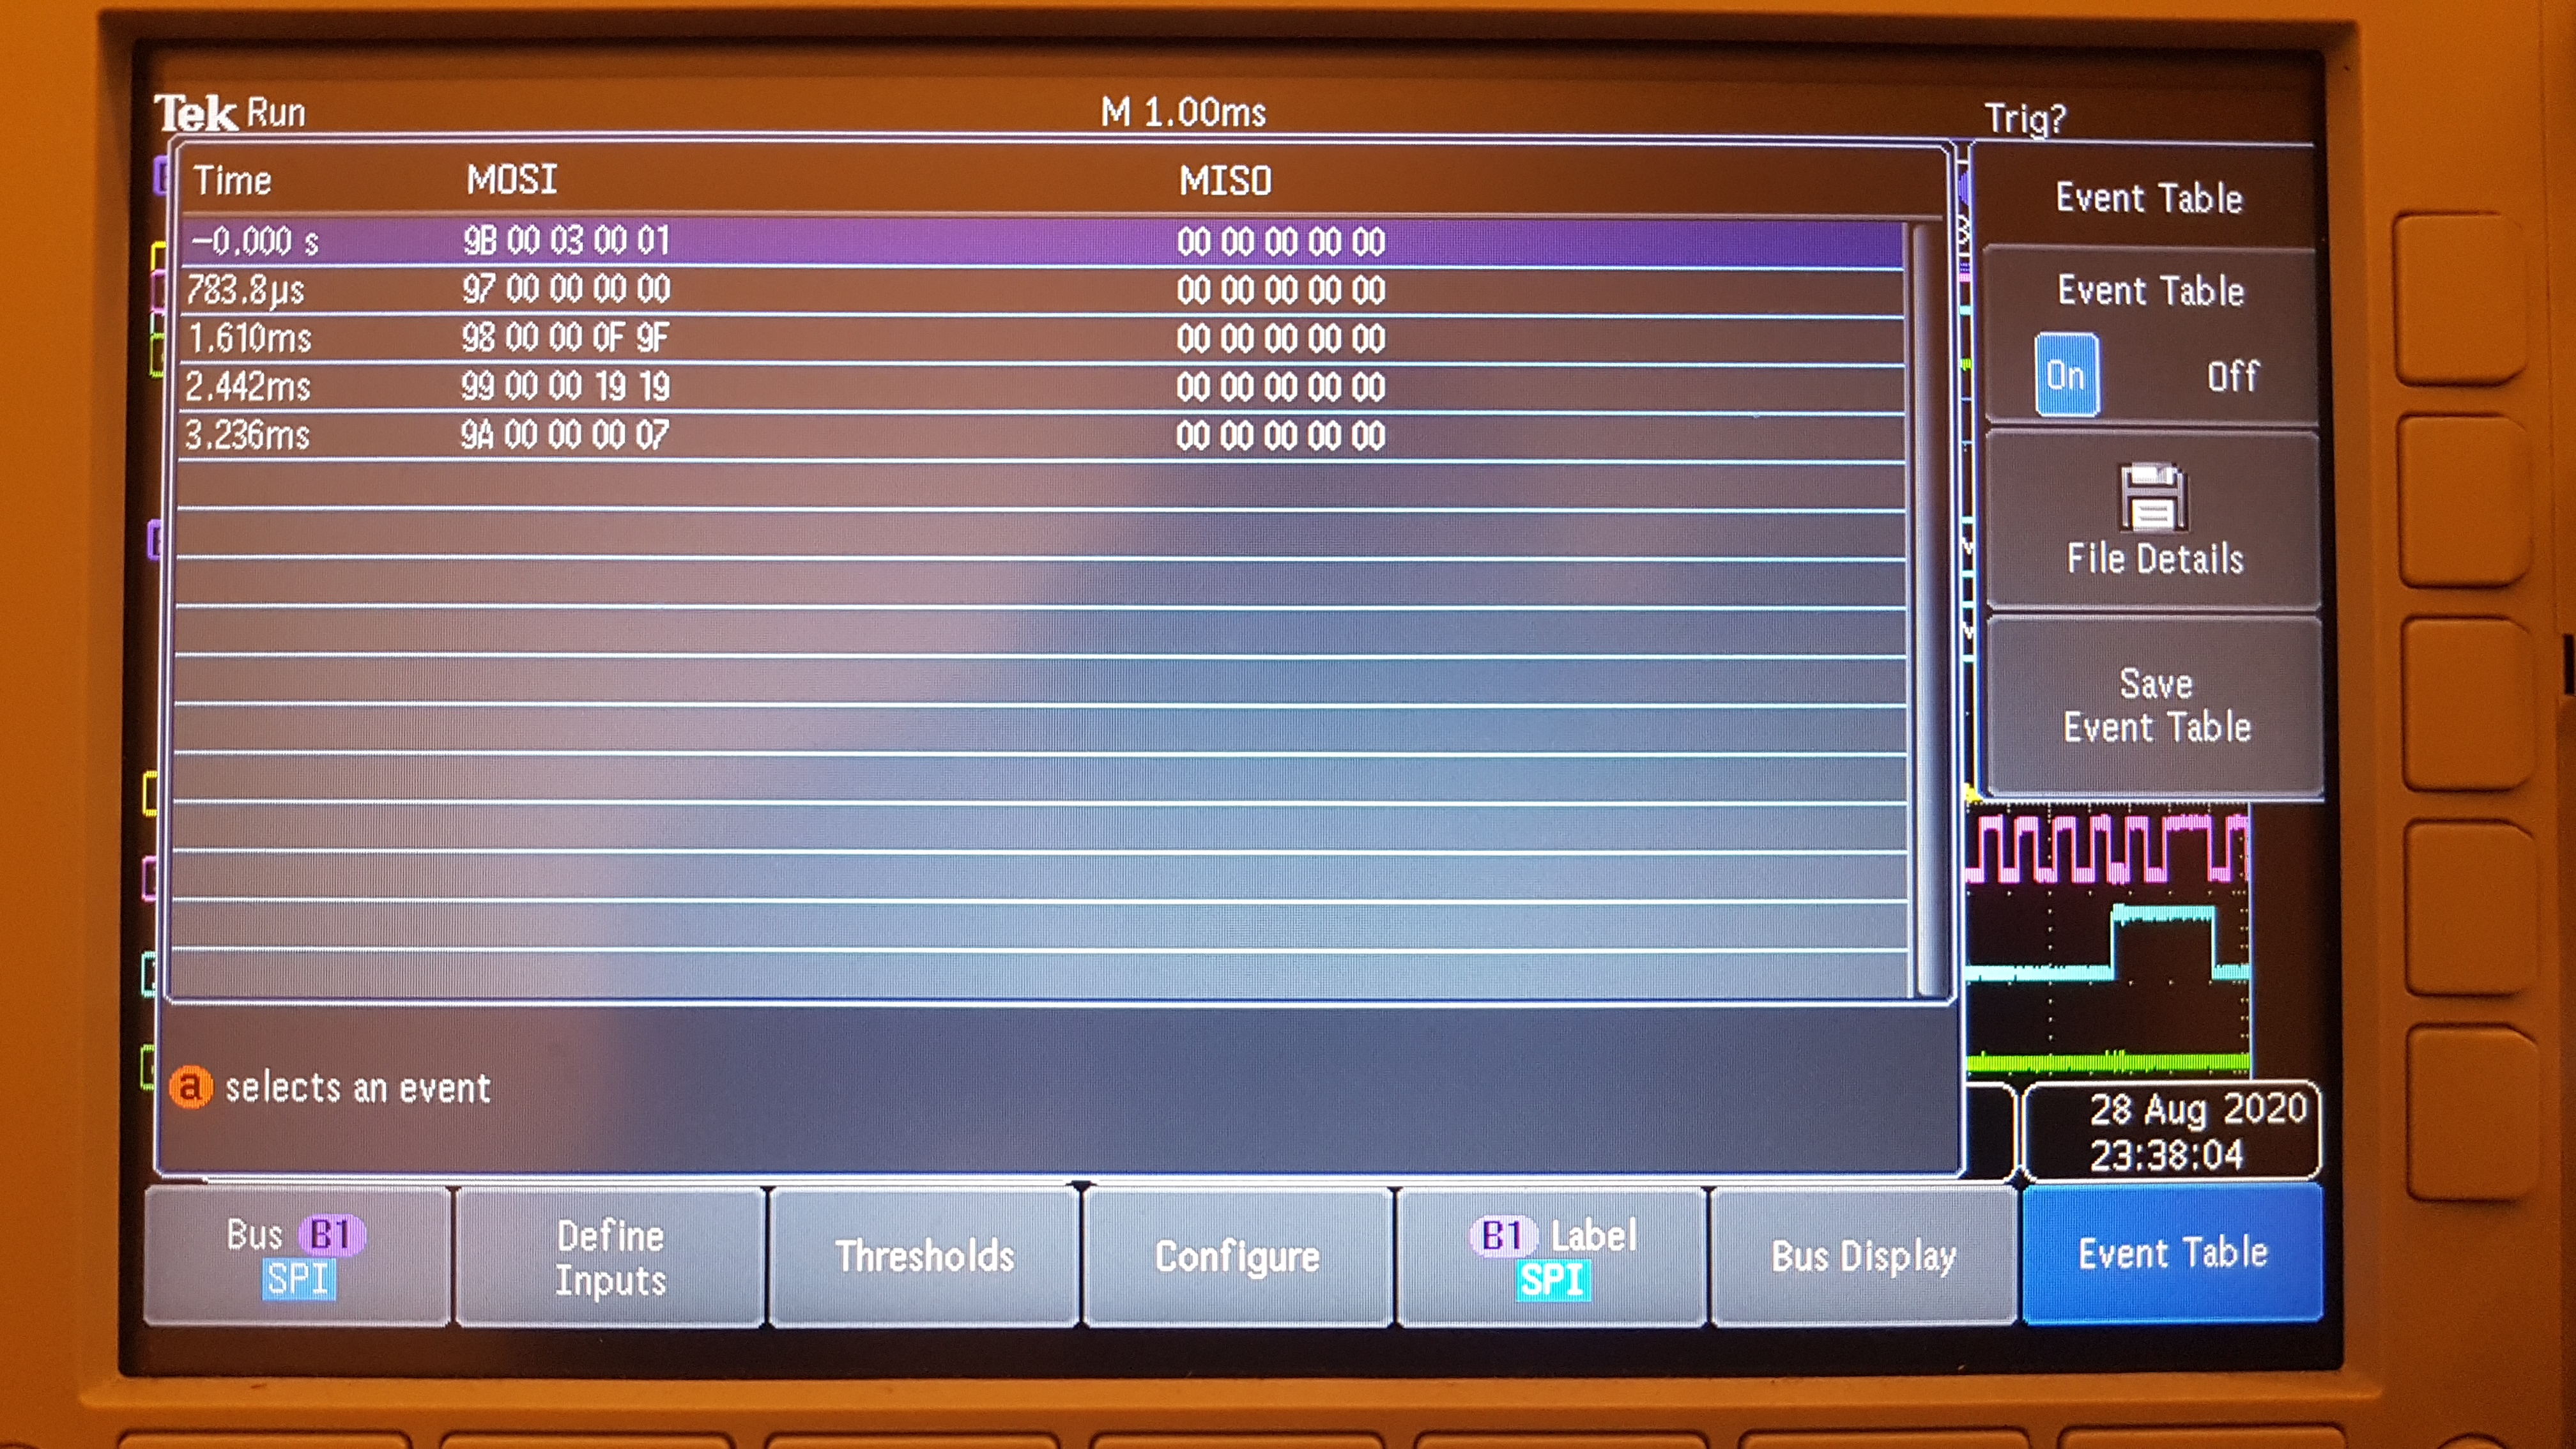
\includegraphics[width = \textwidth]{graphics/TMC4671_TimeTable_Beschreiben1_Bild}
\caption{Event-Table Inbetriebnahme TMC4671.}
\label{fig:TMC4671_TimeTable_Beschreiben1_Bild}
\end{figure}

\begin{figure}[h!]
\center
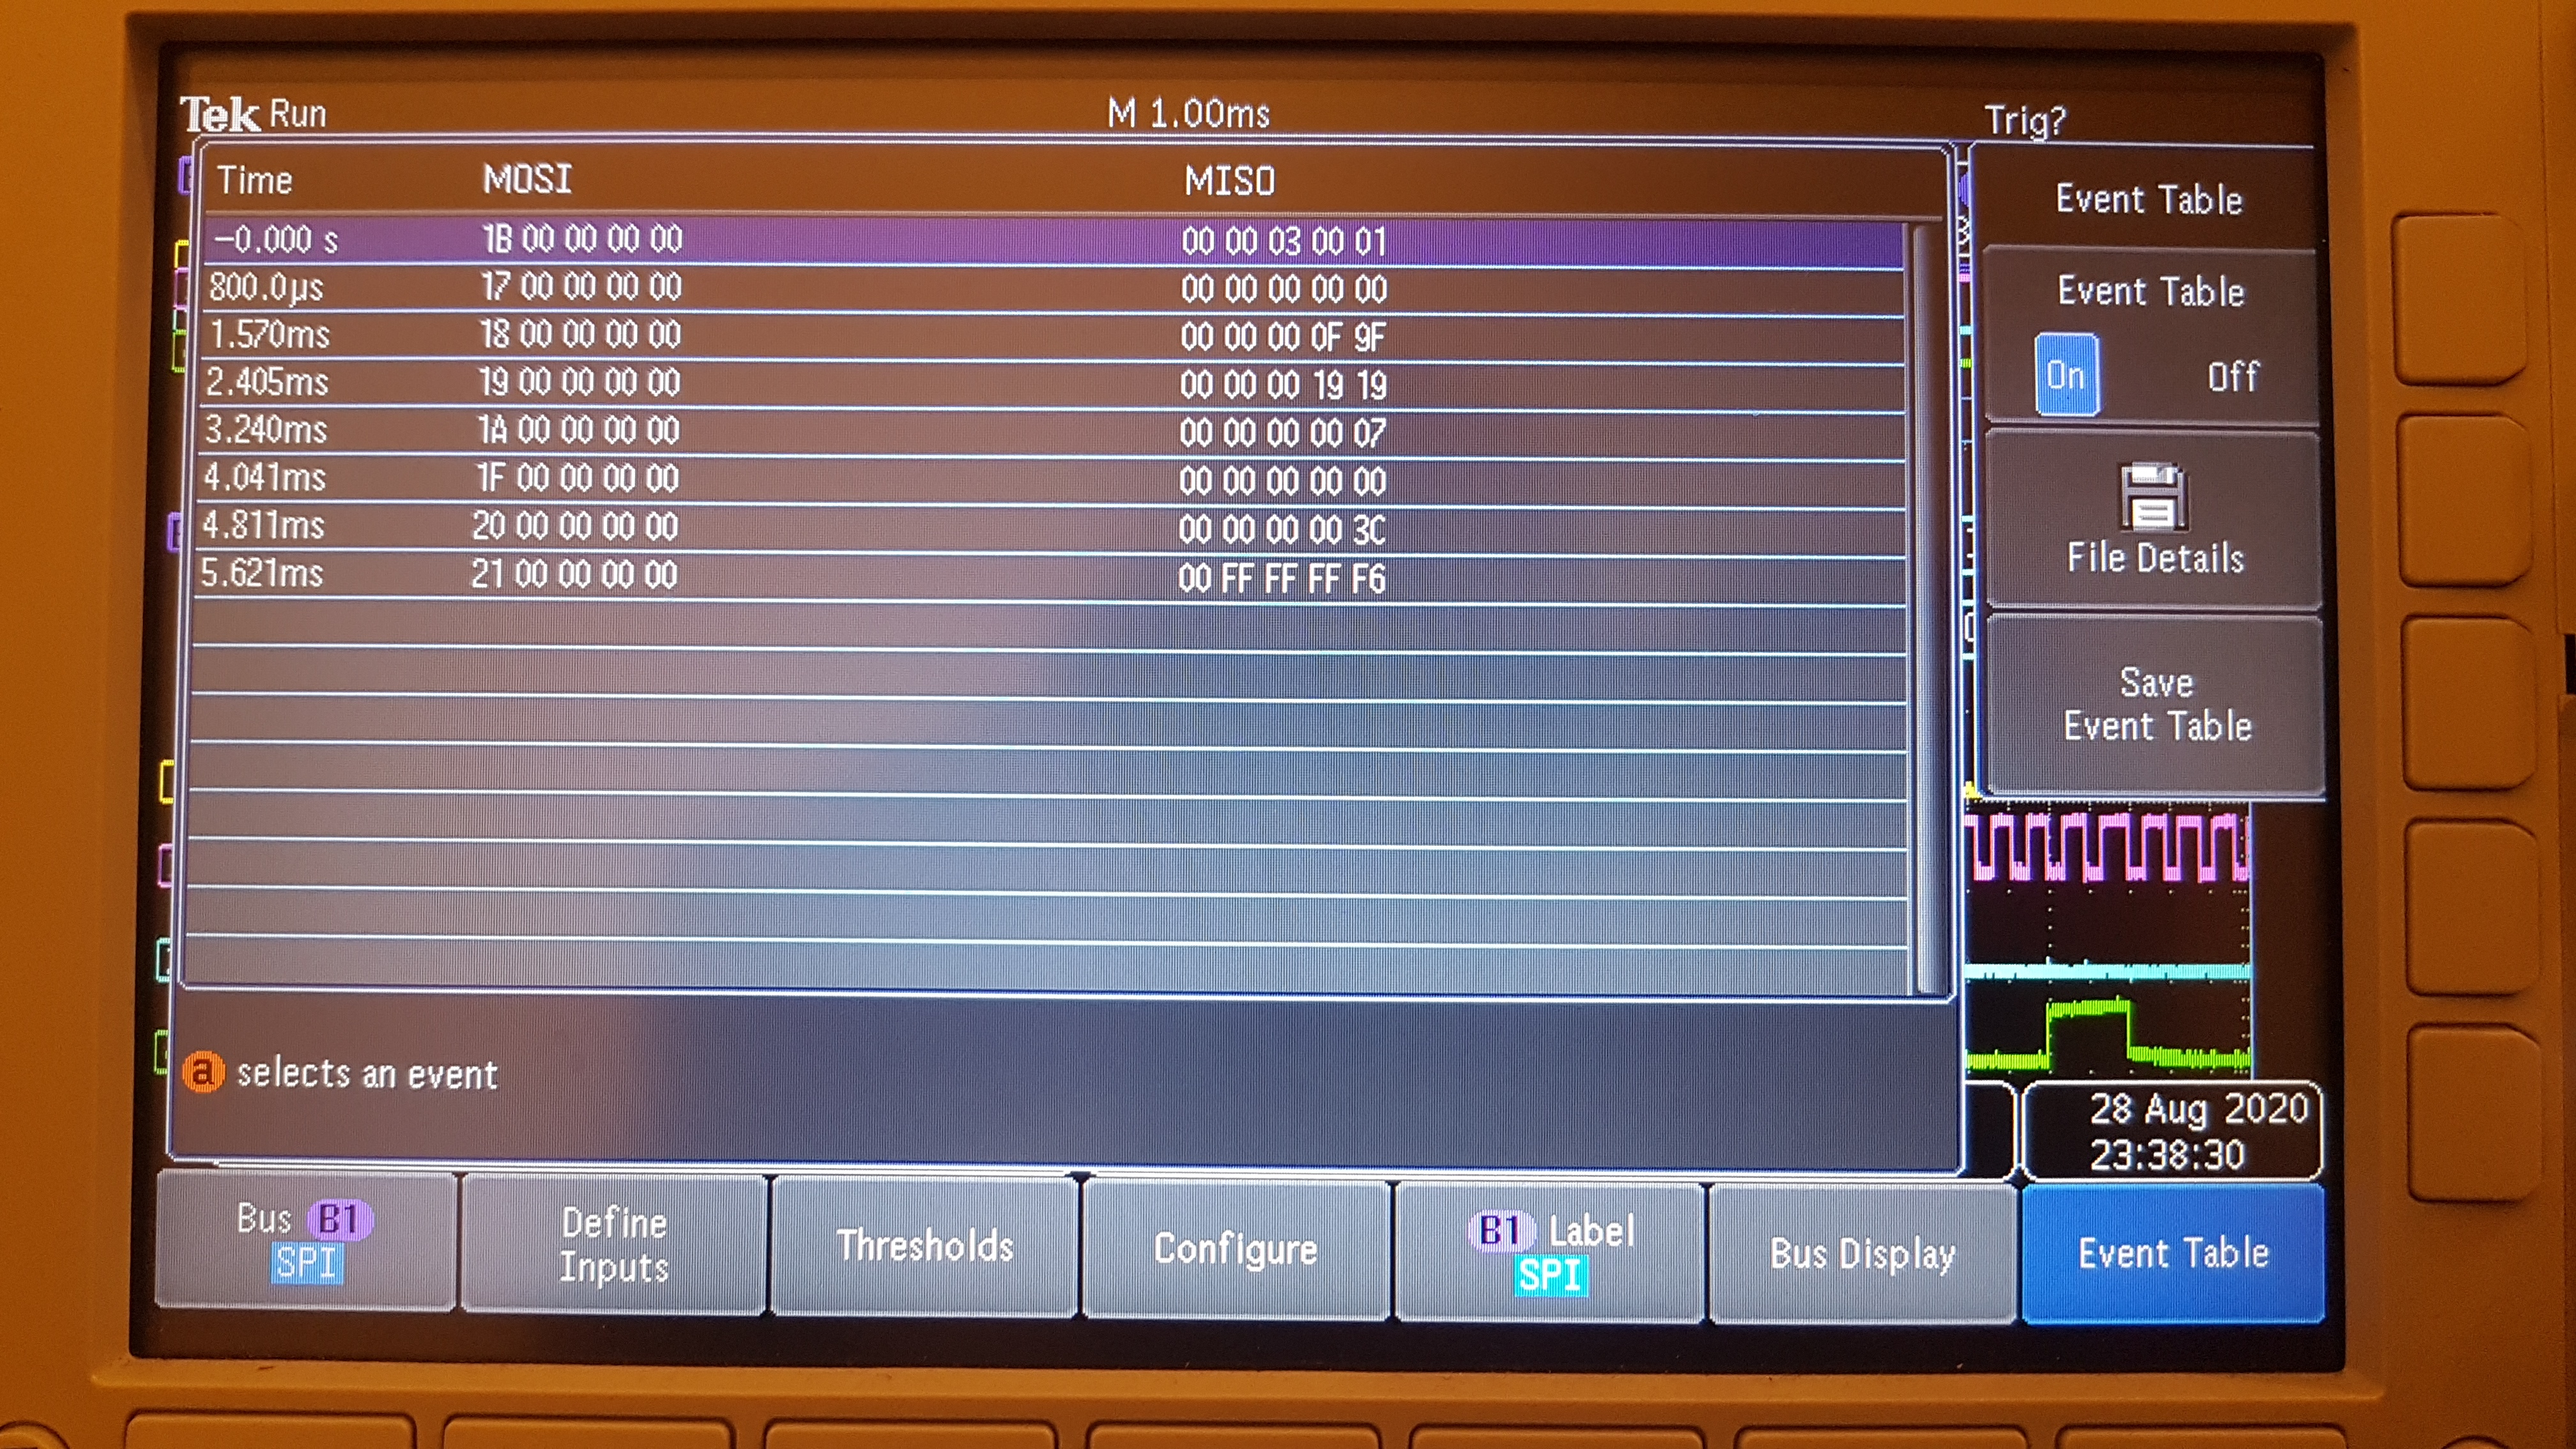
\includegraphics[width = \textwidth]{graphics/TMC4671_TimeTable_Lesen_Bild}
\caption{Event-Table Inbetriebnahme TMC4671.}
\label{fig:TMC4671_TimeTable_Lesen_Bild}
\end{figure}

\newpage

\subsubsection{Inbetriebnahme Gate-Ctrl}\label{Appendix:TMC4671_Gate_Ctrl}

\begin{figure}[h!]
\center
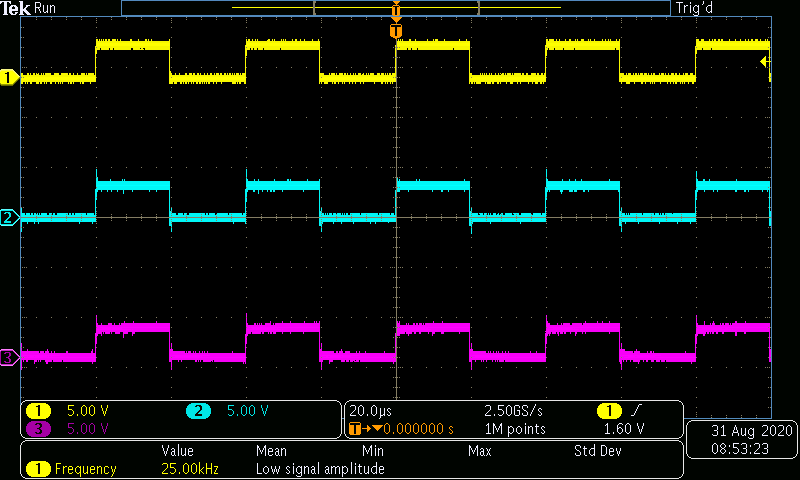
\includegraphics[width = \textwidth]{graphics/TMC4671_Gate_Signal_H}
\caption{Steuersignale PWM 48V. Gelb = U, Blau = V, Magenta = W}
\label{fig:TMC4671_Gate_Signal_H}
\end{figure}

\begin{figure}[h!]
\center
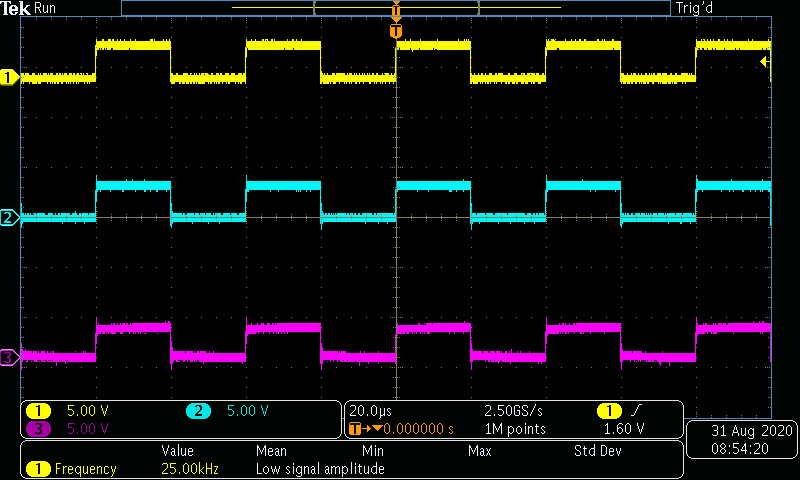
\includegraphics[width = \textwidth]{graphics/TMC4671_Gate_Signal_L}
\caption{Steuersignale PWM 0V. Gelb = U, Blau = V, Magenta = W}
\label{fig:TMC4671_Gate_Signal_L}
\end{figure}

\newpage

\section{TMC6200}\label{Appendix:TMC6200}

\subsection{Standard-Schaltkreis TMC6200}

\begin{figure}[h!]
	\centering
	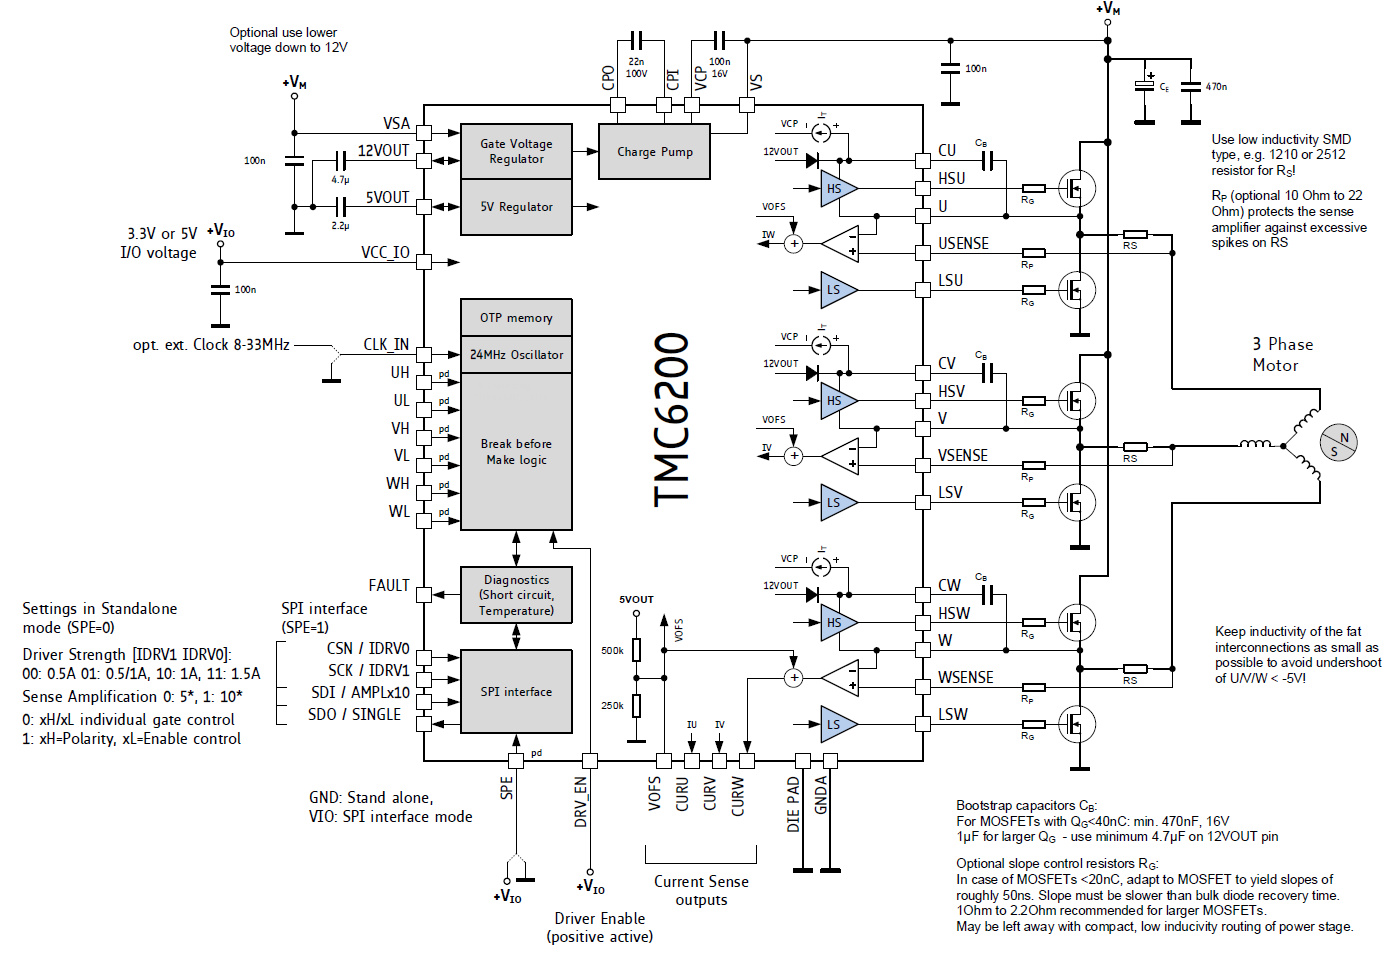
\includegraphics[width=0.8\textwidth]{graphics/Standard_Application_Cirquit_TMC6200.png}
	\caption{Standard-Anwendungs-Schaltung TMC6200.}
	\label{fig:Schaltung_TMC6200}
\end{figure}

\subsection{Blockdiagramm TMC6200}

\begin{figure}[h!]
	\centering
	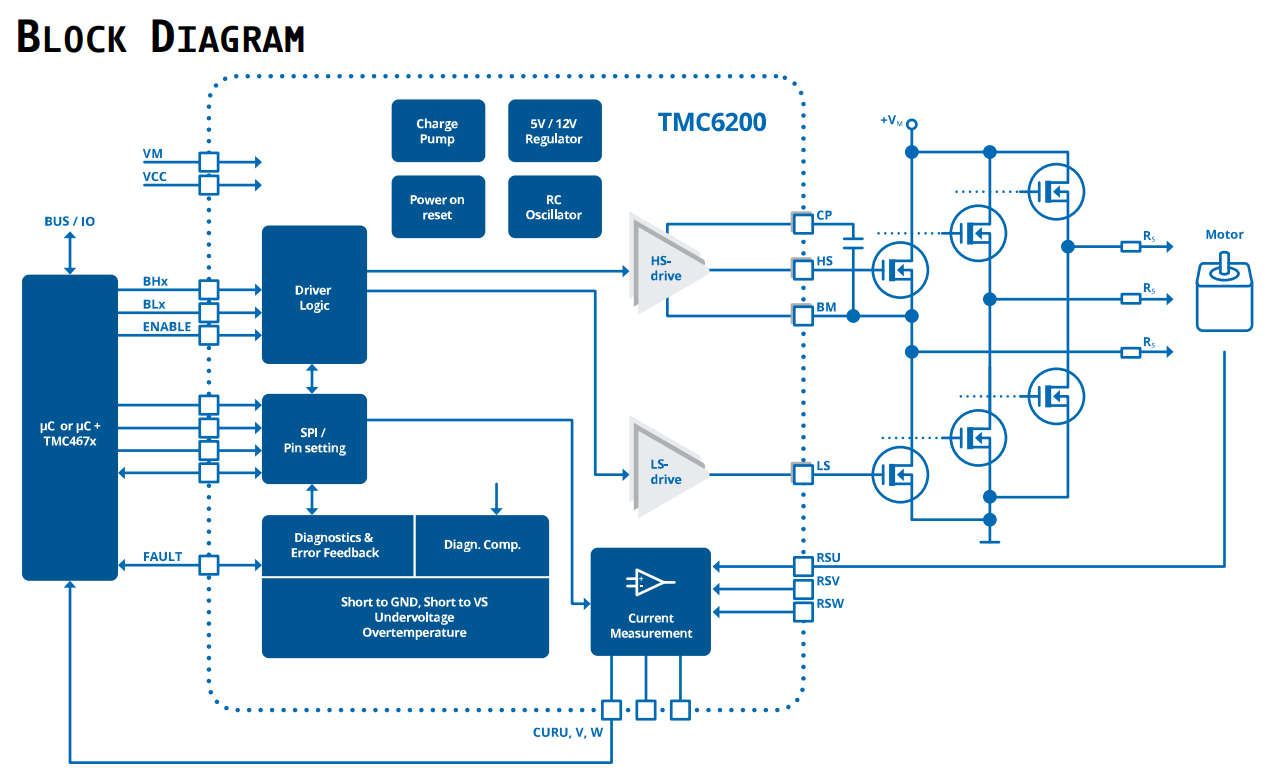
\includegraphics[width=0.8\textwidth]{graphics/Blockdiagramm_TMC6200.png}
	\caption{Blockdiagramm TMC6200.}
	\label{fig:Blockdiagramm_TMC6200}
\end{figure}

\newpage

\subsection{Verstärkungsfaktor, Strommessung, Strommesswiderstand}

\begin{figure}[h!]
	\centering
	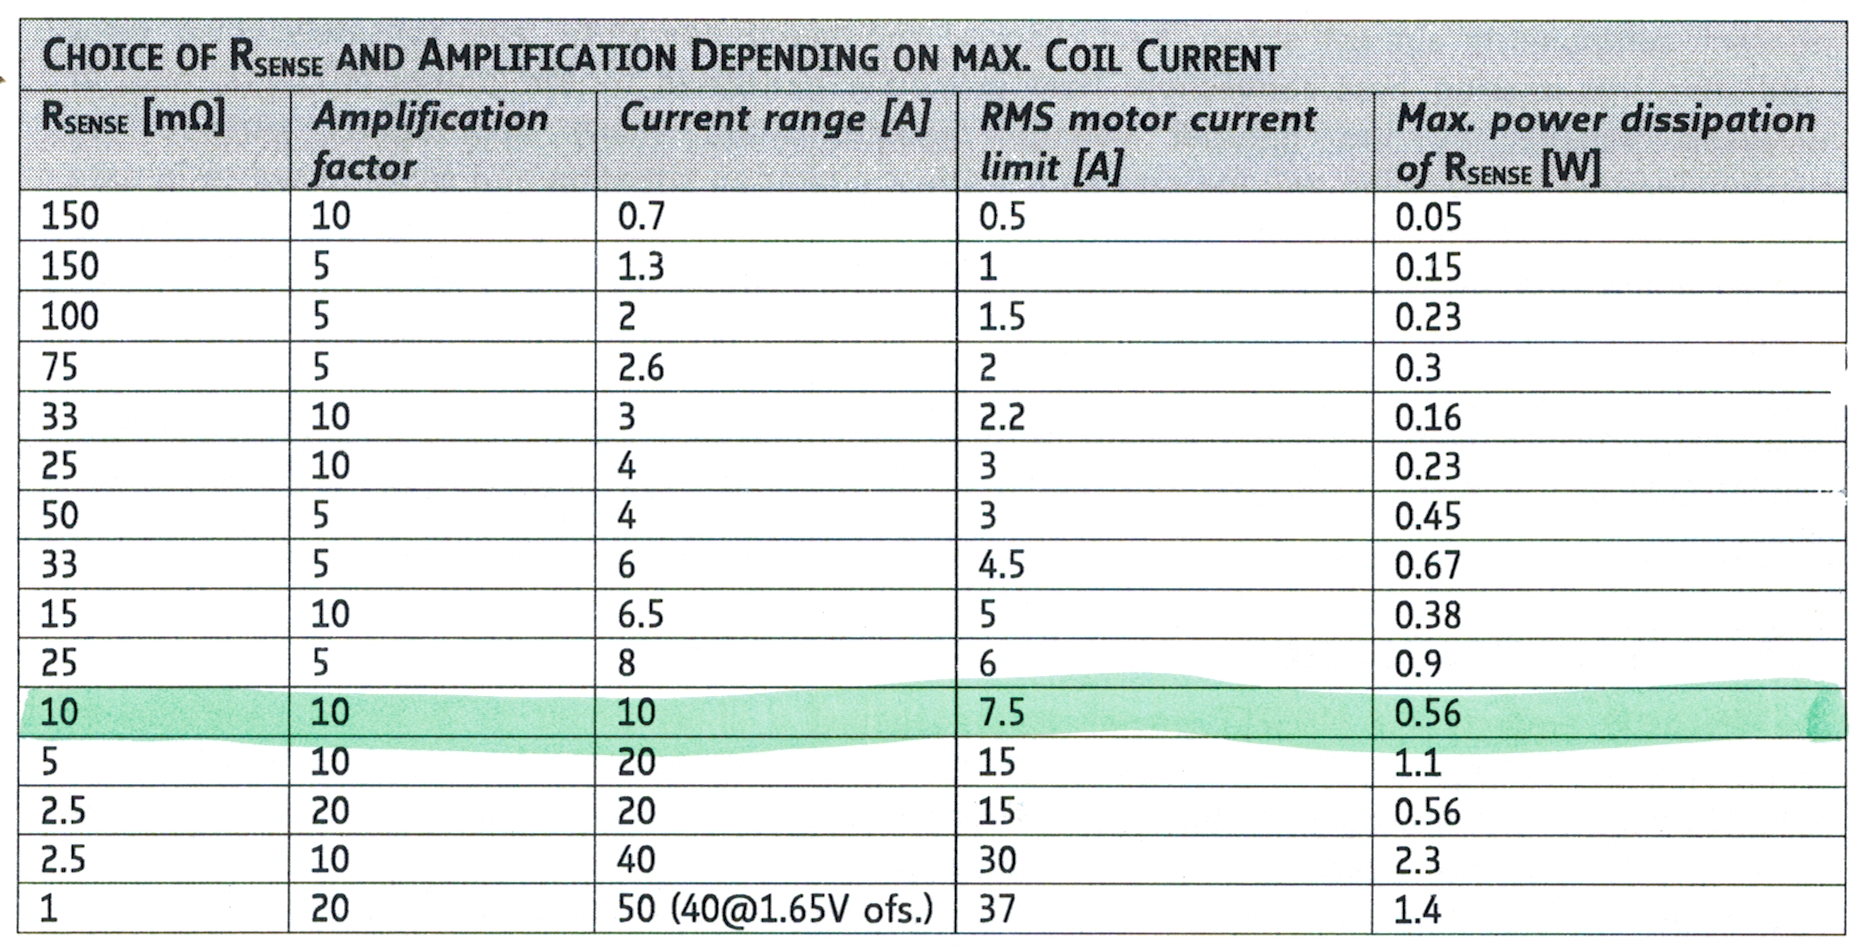
\includegraphics[width=\textwidth]{graphics/Tabelle_Shunts.png}
	\caption{Tabelle zur Bestimmung des Strommesswiderstandes aus dem Datenblatt von Trinamic.}
	\label{fig:Tabelle_Shunts}
\end{figure}

\subsection{Gate-Vorwiderstand}

\begin{figure}[h!]
	\centering
	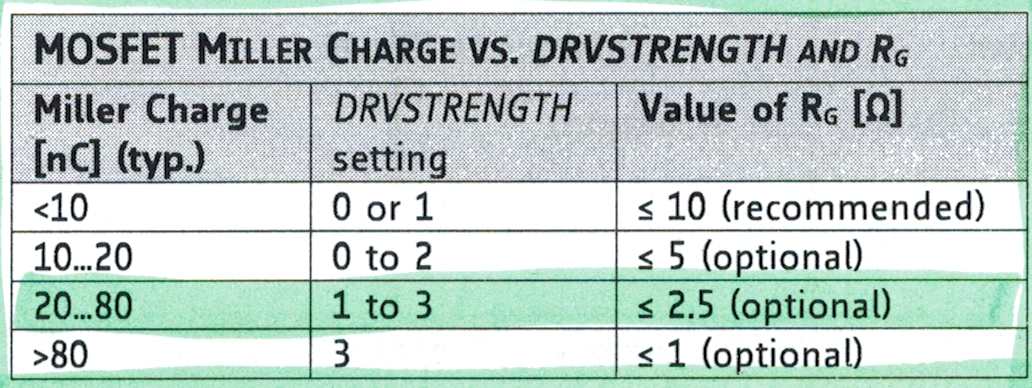
\includegraphics[width=0.5\textwidth]{graphics/Tabelle_Gatewiderstaende.png}
	\caption{Tabelle zur Bestimmung der Gatewiderstände aus dem Datenblatt von Trinamic.}
	\label{fig:Tabelle_Gatewiderstaende}
\end{figure}

\subsection{Externe Gate-Spannungsversorgung}

\begin{figure}[h!]
	\centering
	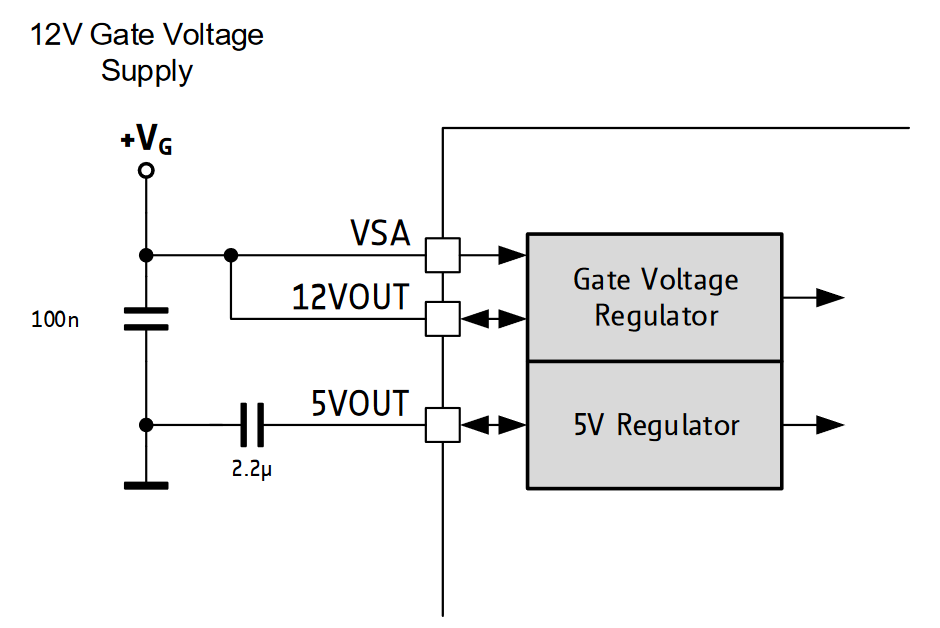
\includegraphics[width=0.4\textwidth]{graphics/Schema_Gate_Treiber_Gatespannung}
	\caption{Schema externe Gate-Spannungsversorgung.}
	\label{fig:Schema_Gate_Treiber_Gatespannung}
\end{figure}

\newpage

\subsection{Inbetriebnahme}

\subsubsection{Inbetriebnahme Setup}\label{Appendix:TMC6200_Setup}

\begin{figure}[h!]
	\centering
	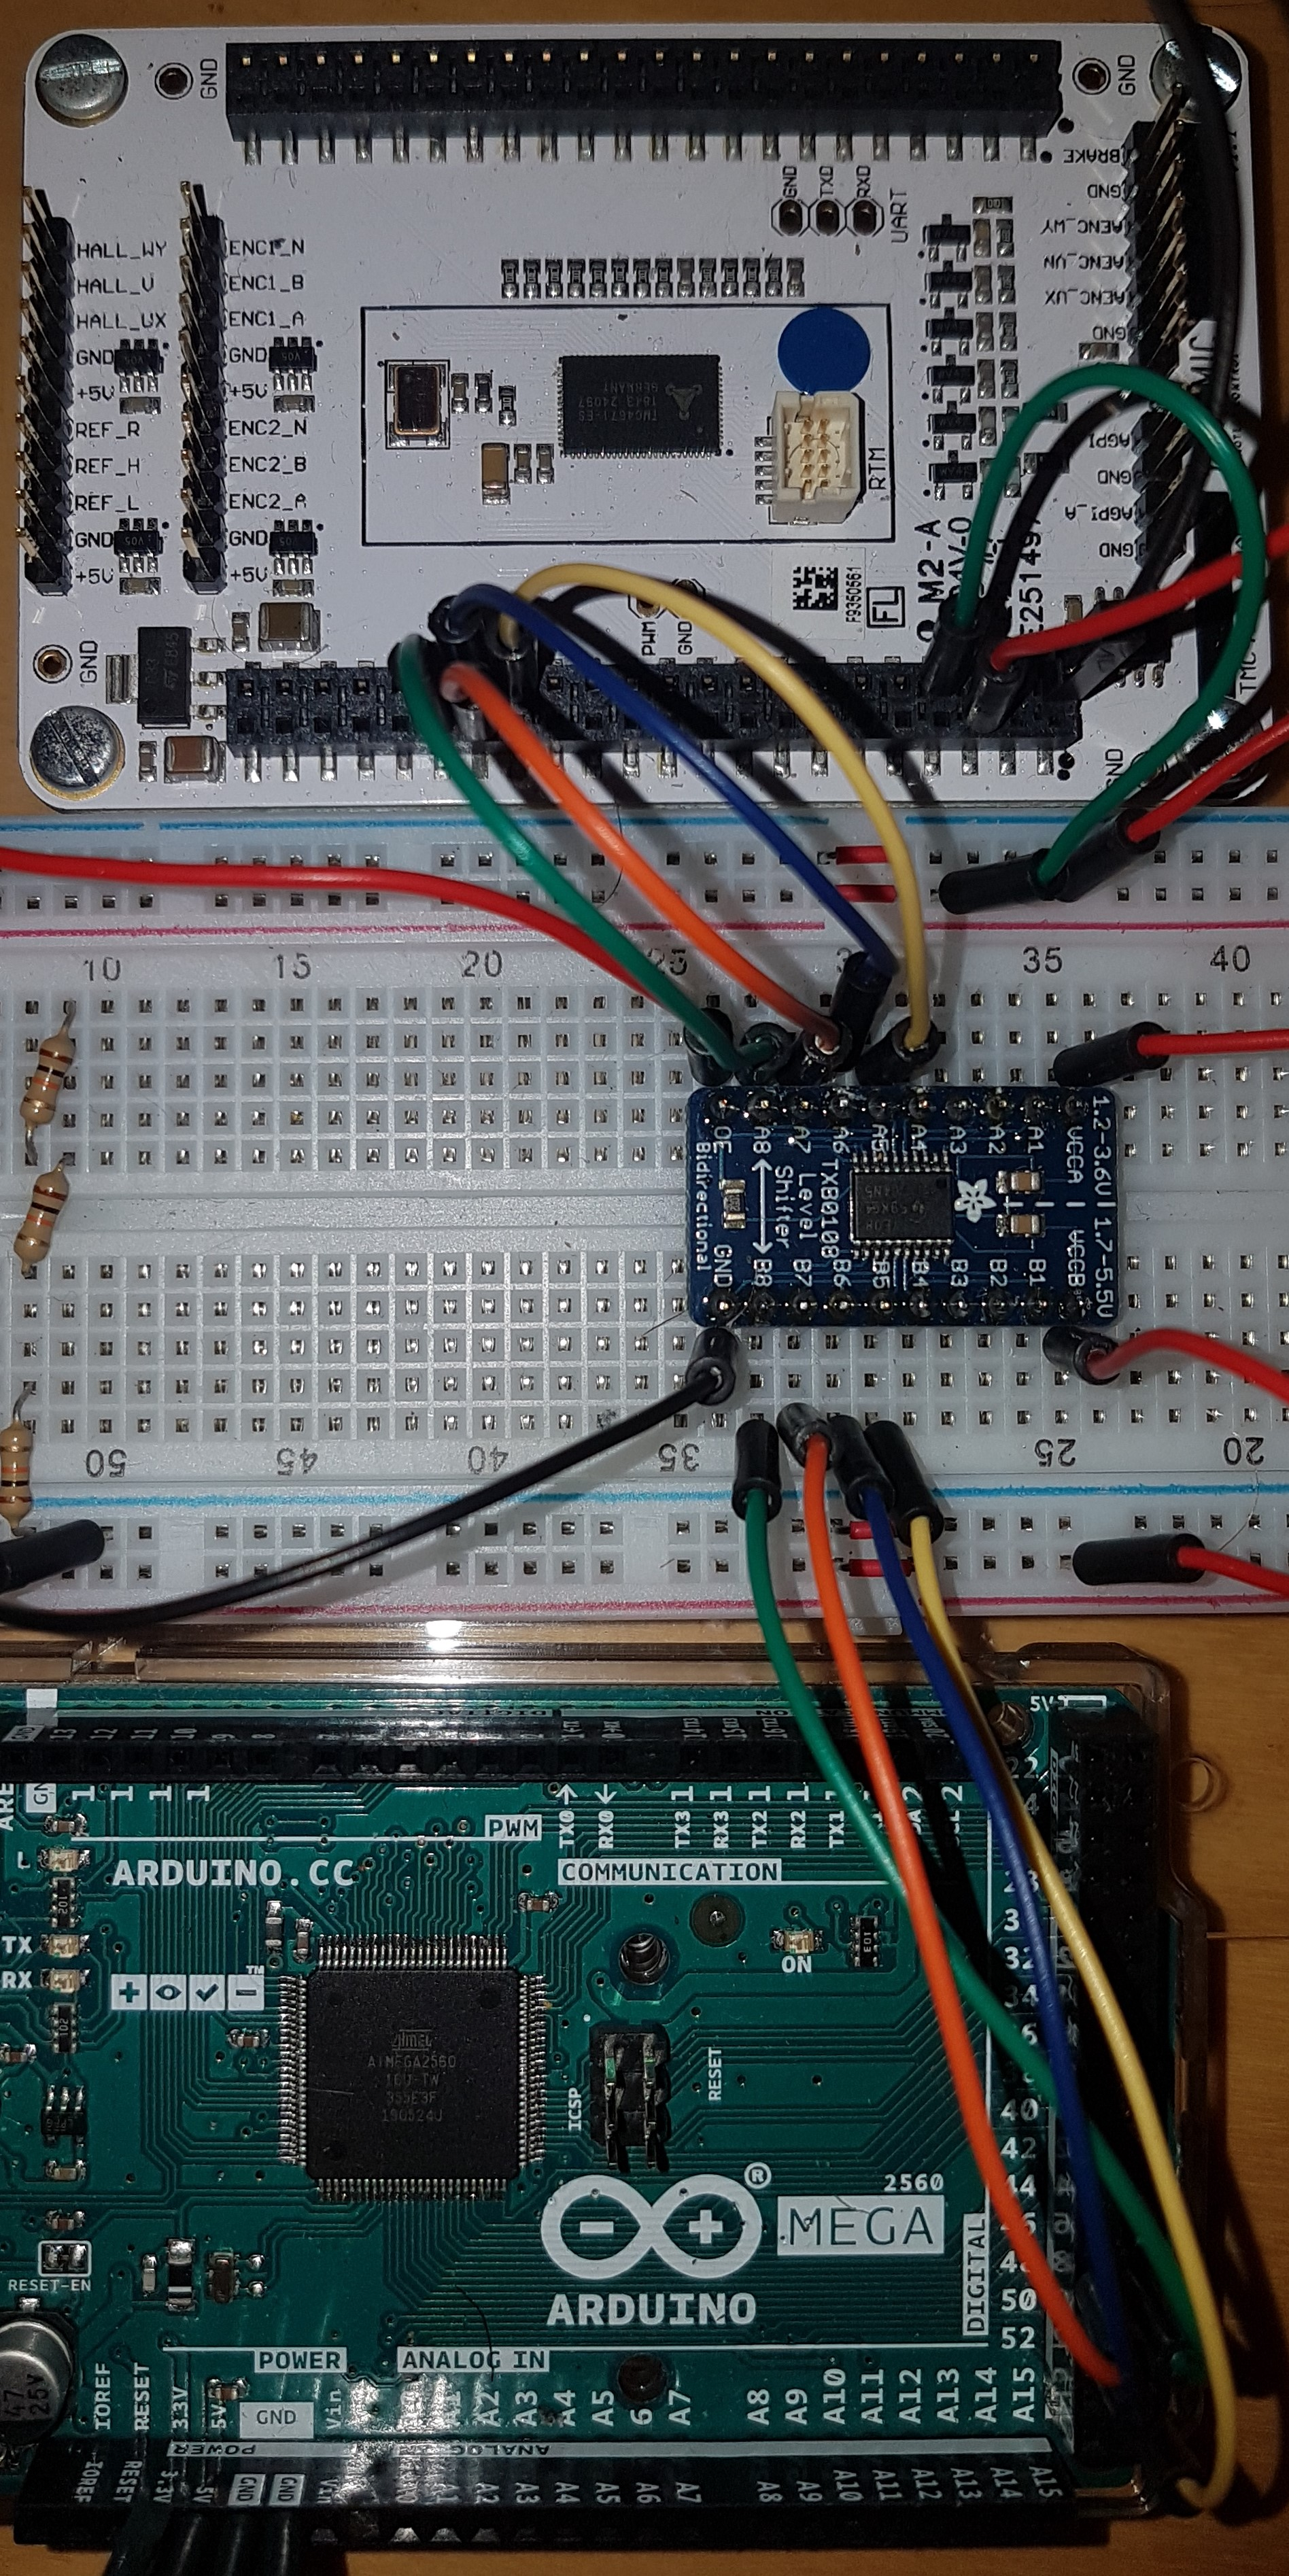
\includegraphics[angle=270,width=\textwidth]{graphics/1_komplett}
	\caption{Gesamtansicht Setup.}
	\label{fig:1_komplett}
\end{figure}

\begin{figure}[h!]
	\centering
	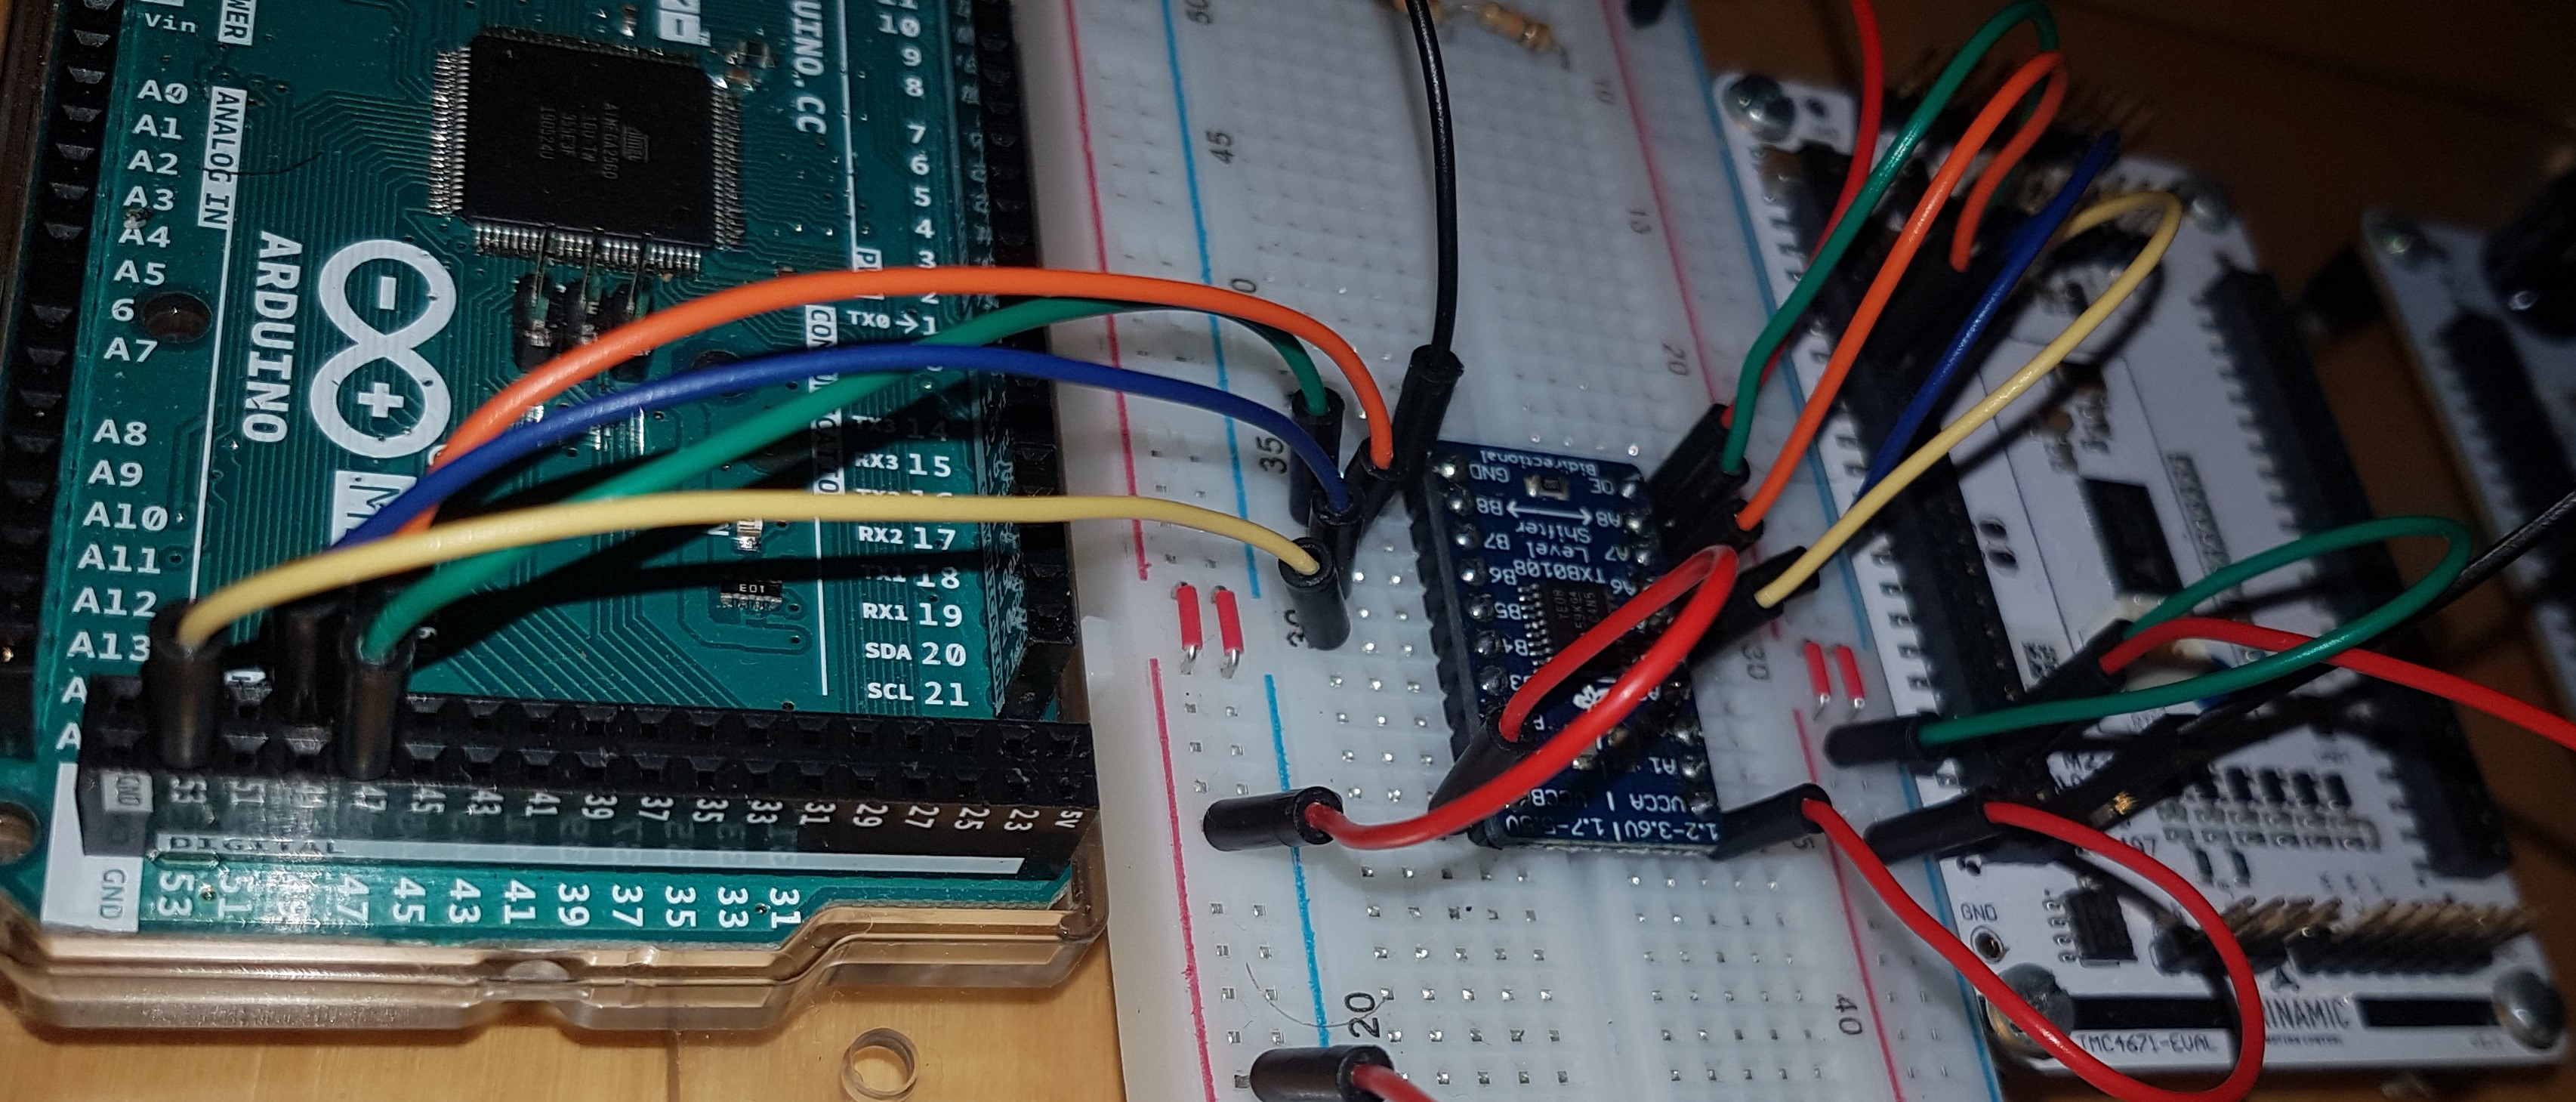
\includegraphics[width=\textwidth]{graphics/1_Arduino}
	\caption{Setup mit Fokus auf Arduino.}
	\label{fig:1_Arduino}
\end{figure}

\newpage

\begin{figure}[h!]
	\centering
	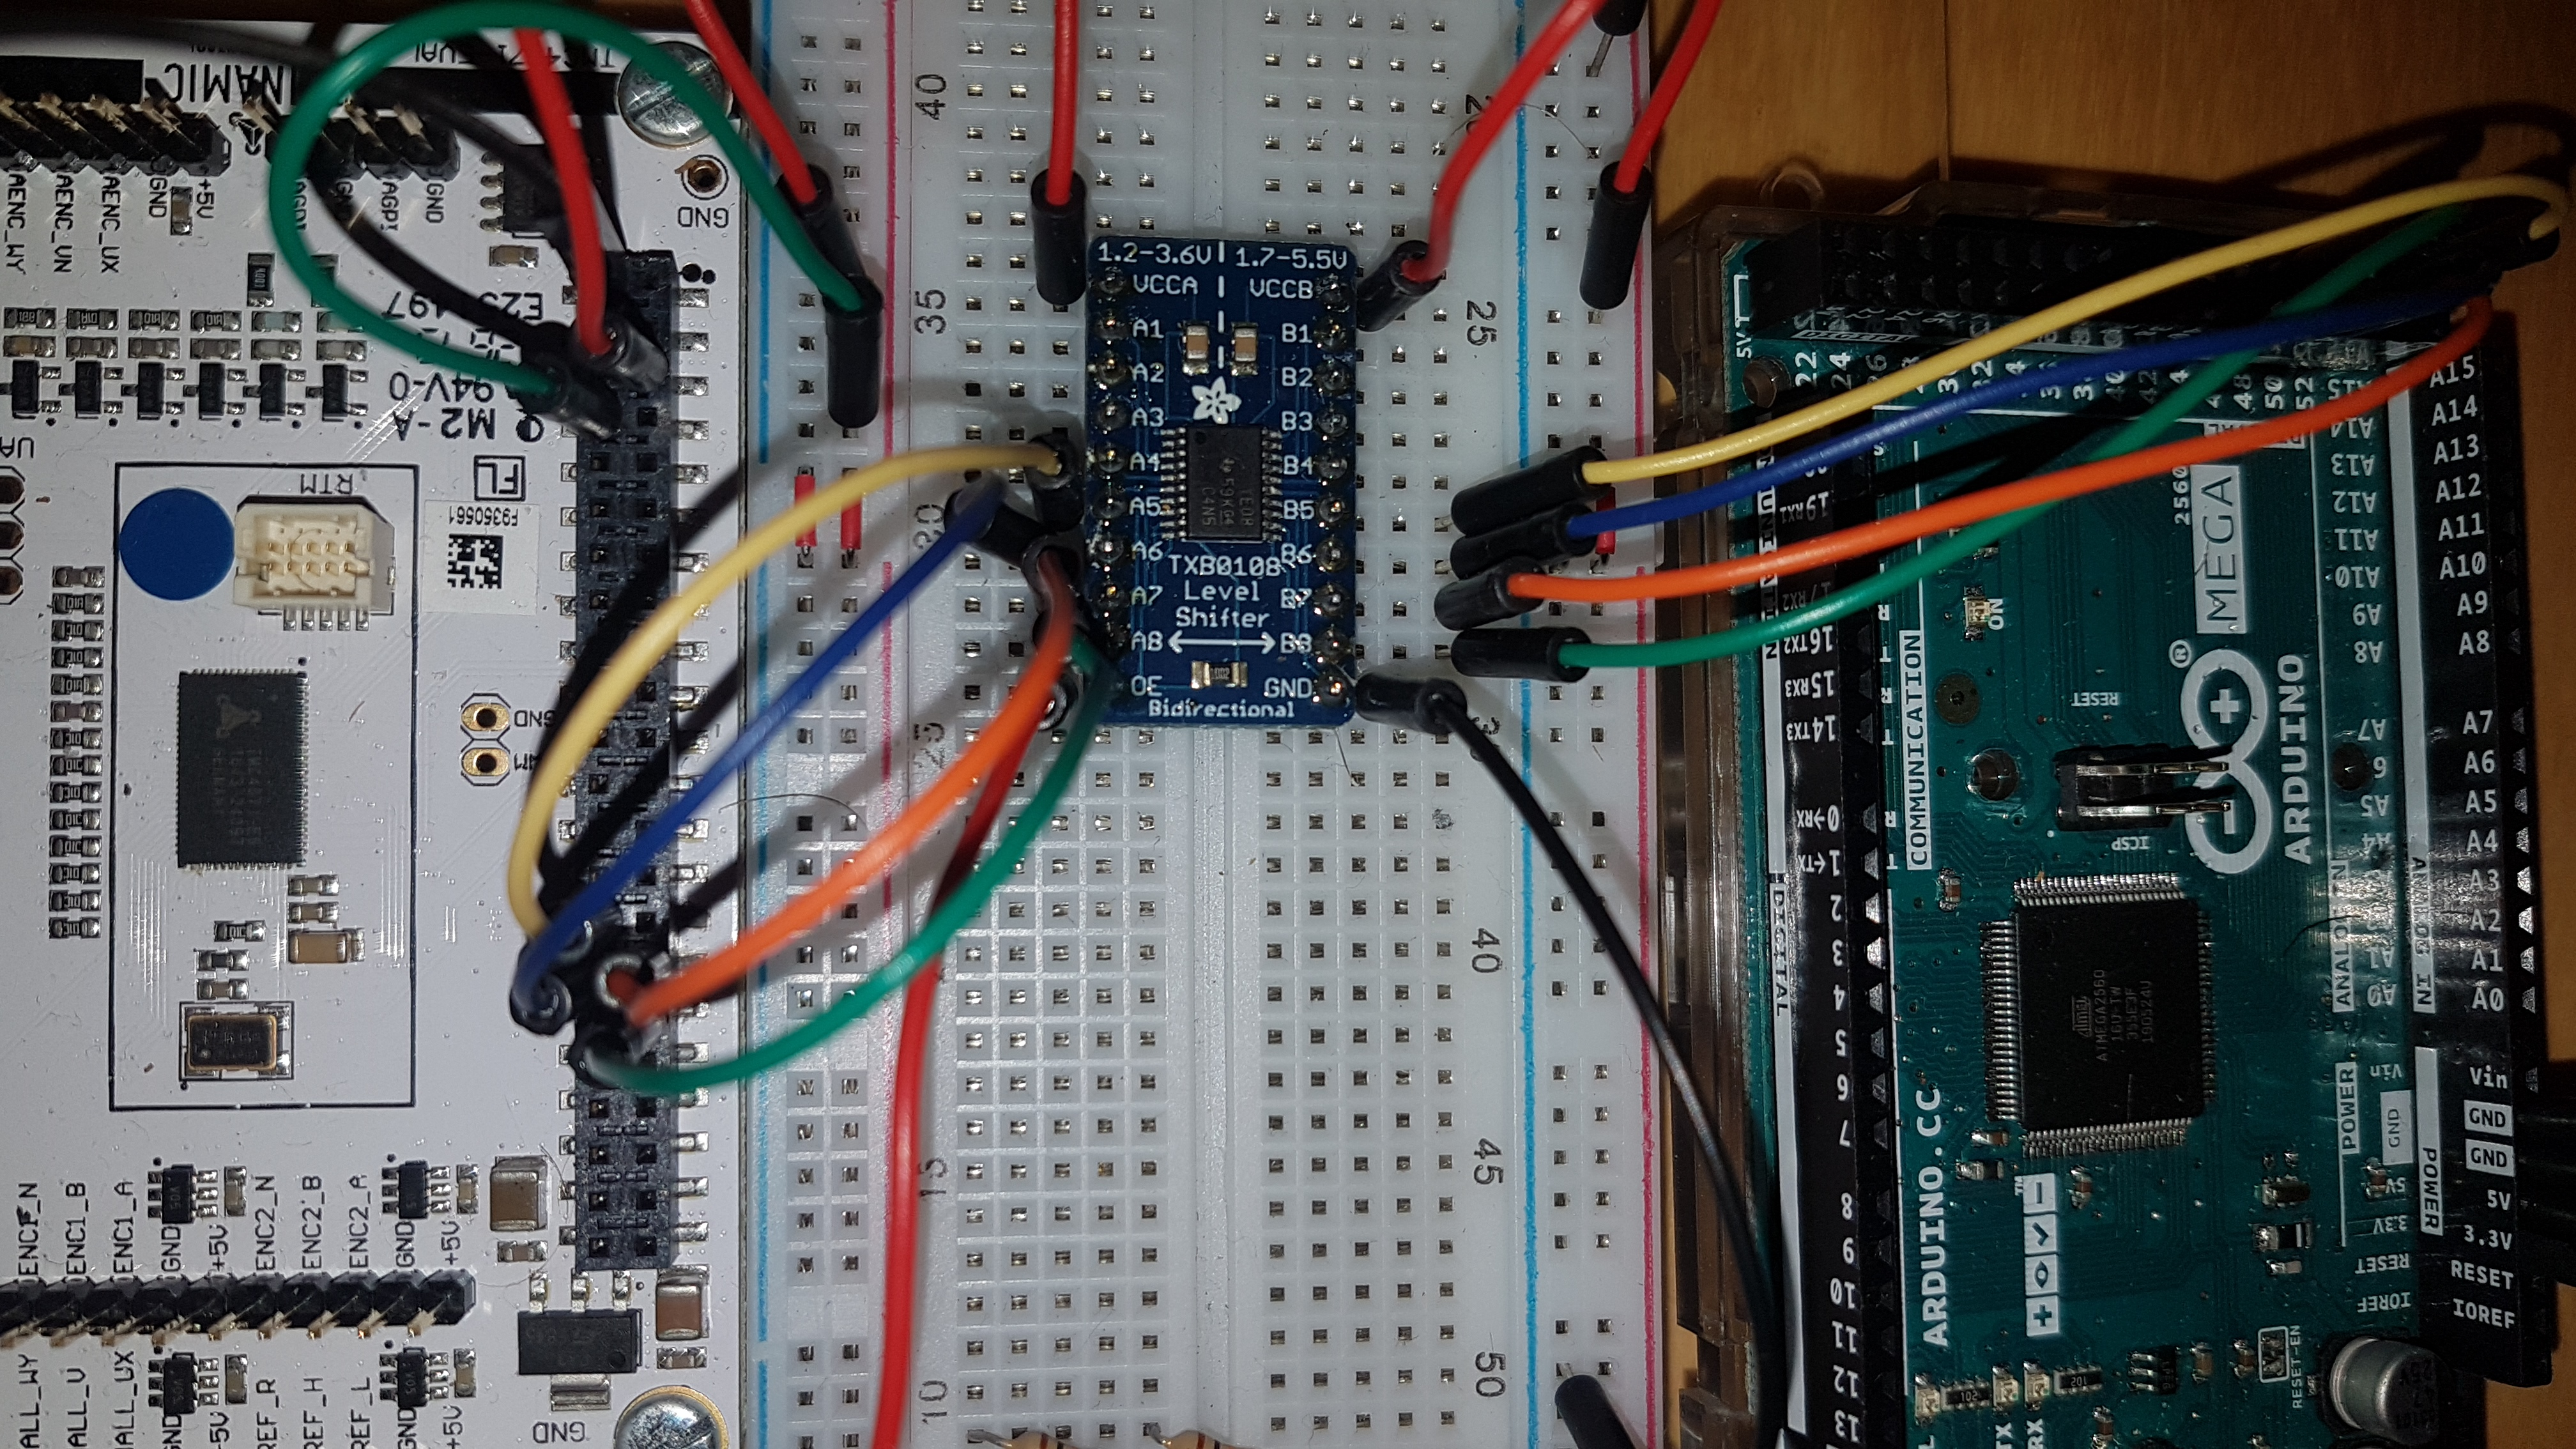
\includegraphics[angle=180,width=\textwidth]{graphics/1_EVAL}
	\caption{Setup mit Fokus auf TMC4674-EVAL.}
	\label{fig:1_EVAL}
\end{figure}

\subsubsection{Inbetriebnahme SPI-Kommunikation}\label{Appendix:TMC6200_SPI}

\begin{figure}[h!]
\center
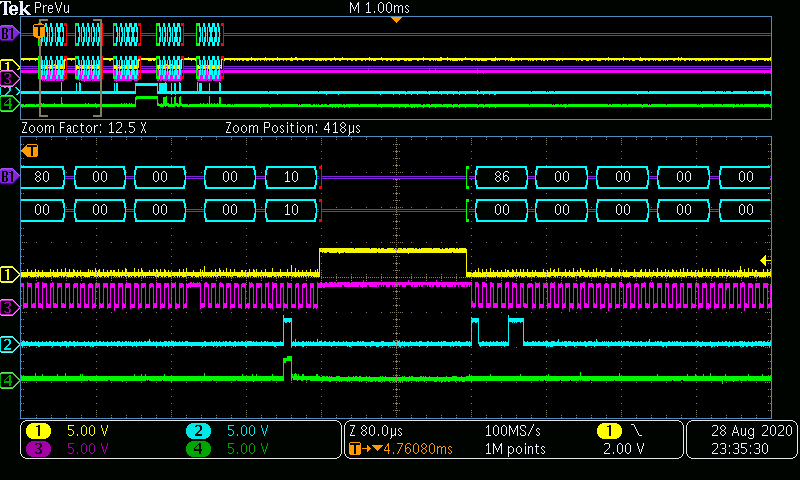
\includegraphics[width = \textwidth]{graphics/TMC6200_Beschreiben2}
\caption{SPI-Übertragung Write 1.}
\label{fig:TMC6200_Beschreiben2}
\end{figure}

\newpage

\begin{figure}[h!]
\center
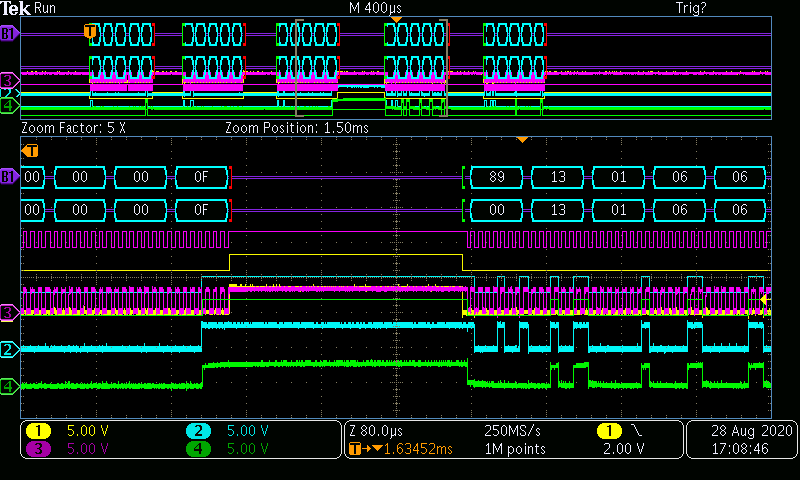
\includegraphics[width = \textwidth]{graphics/TMC6200_Beschreiben}
\caption{SPI-Übertragung Write 2.}
\label{fig:TMC6200_Beschreiben}
\end{figure}

\begin{figure}[h!]
\center
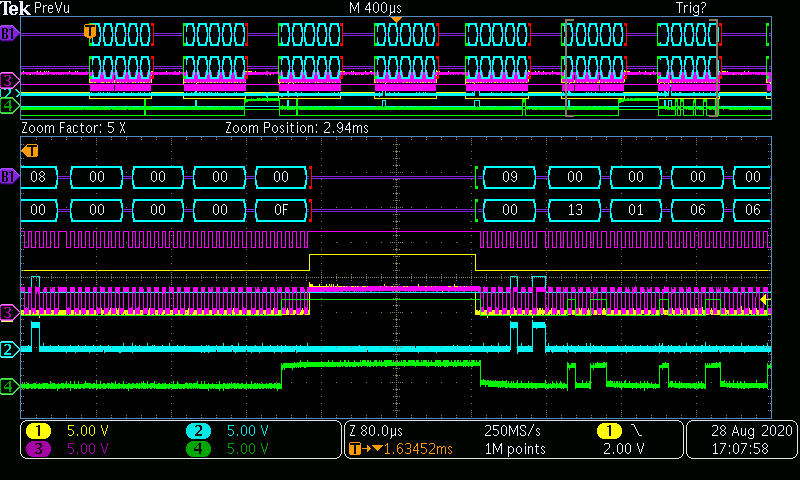
\includegraphics[width = \textwidth]{graphics/TMC6200_Lesen}
\caption{SPI-Übertragung Read.}
\label{fig:TMC6200_Lesen}
\end{figure}

\newpage

\begin{figure}[h!]
\center
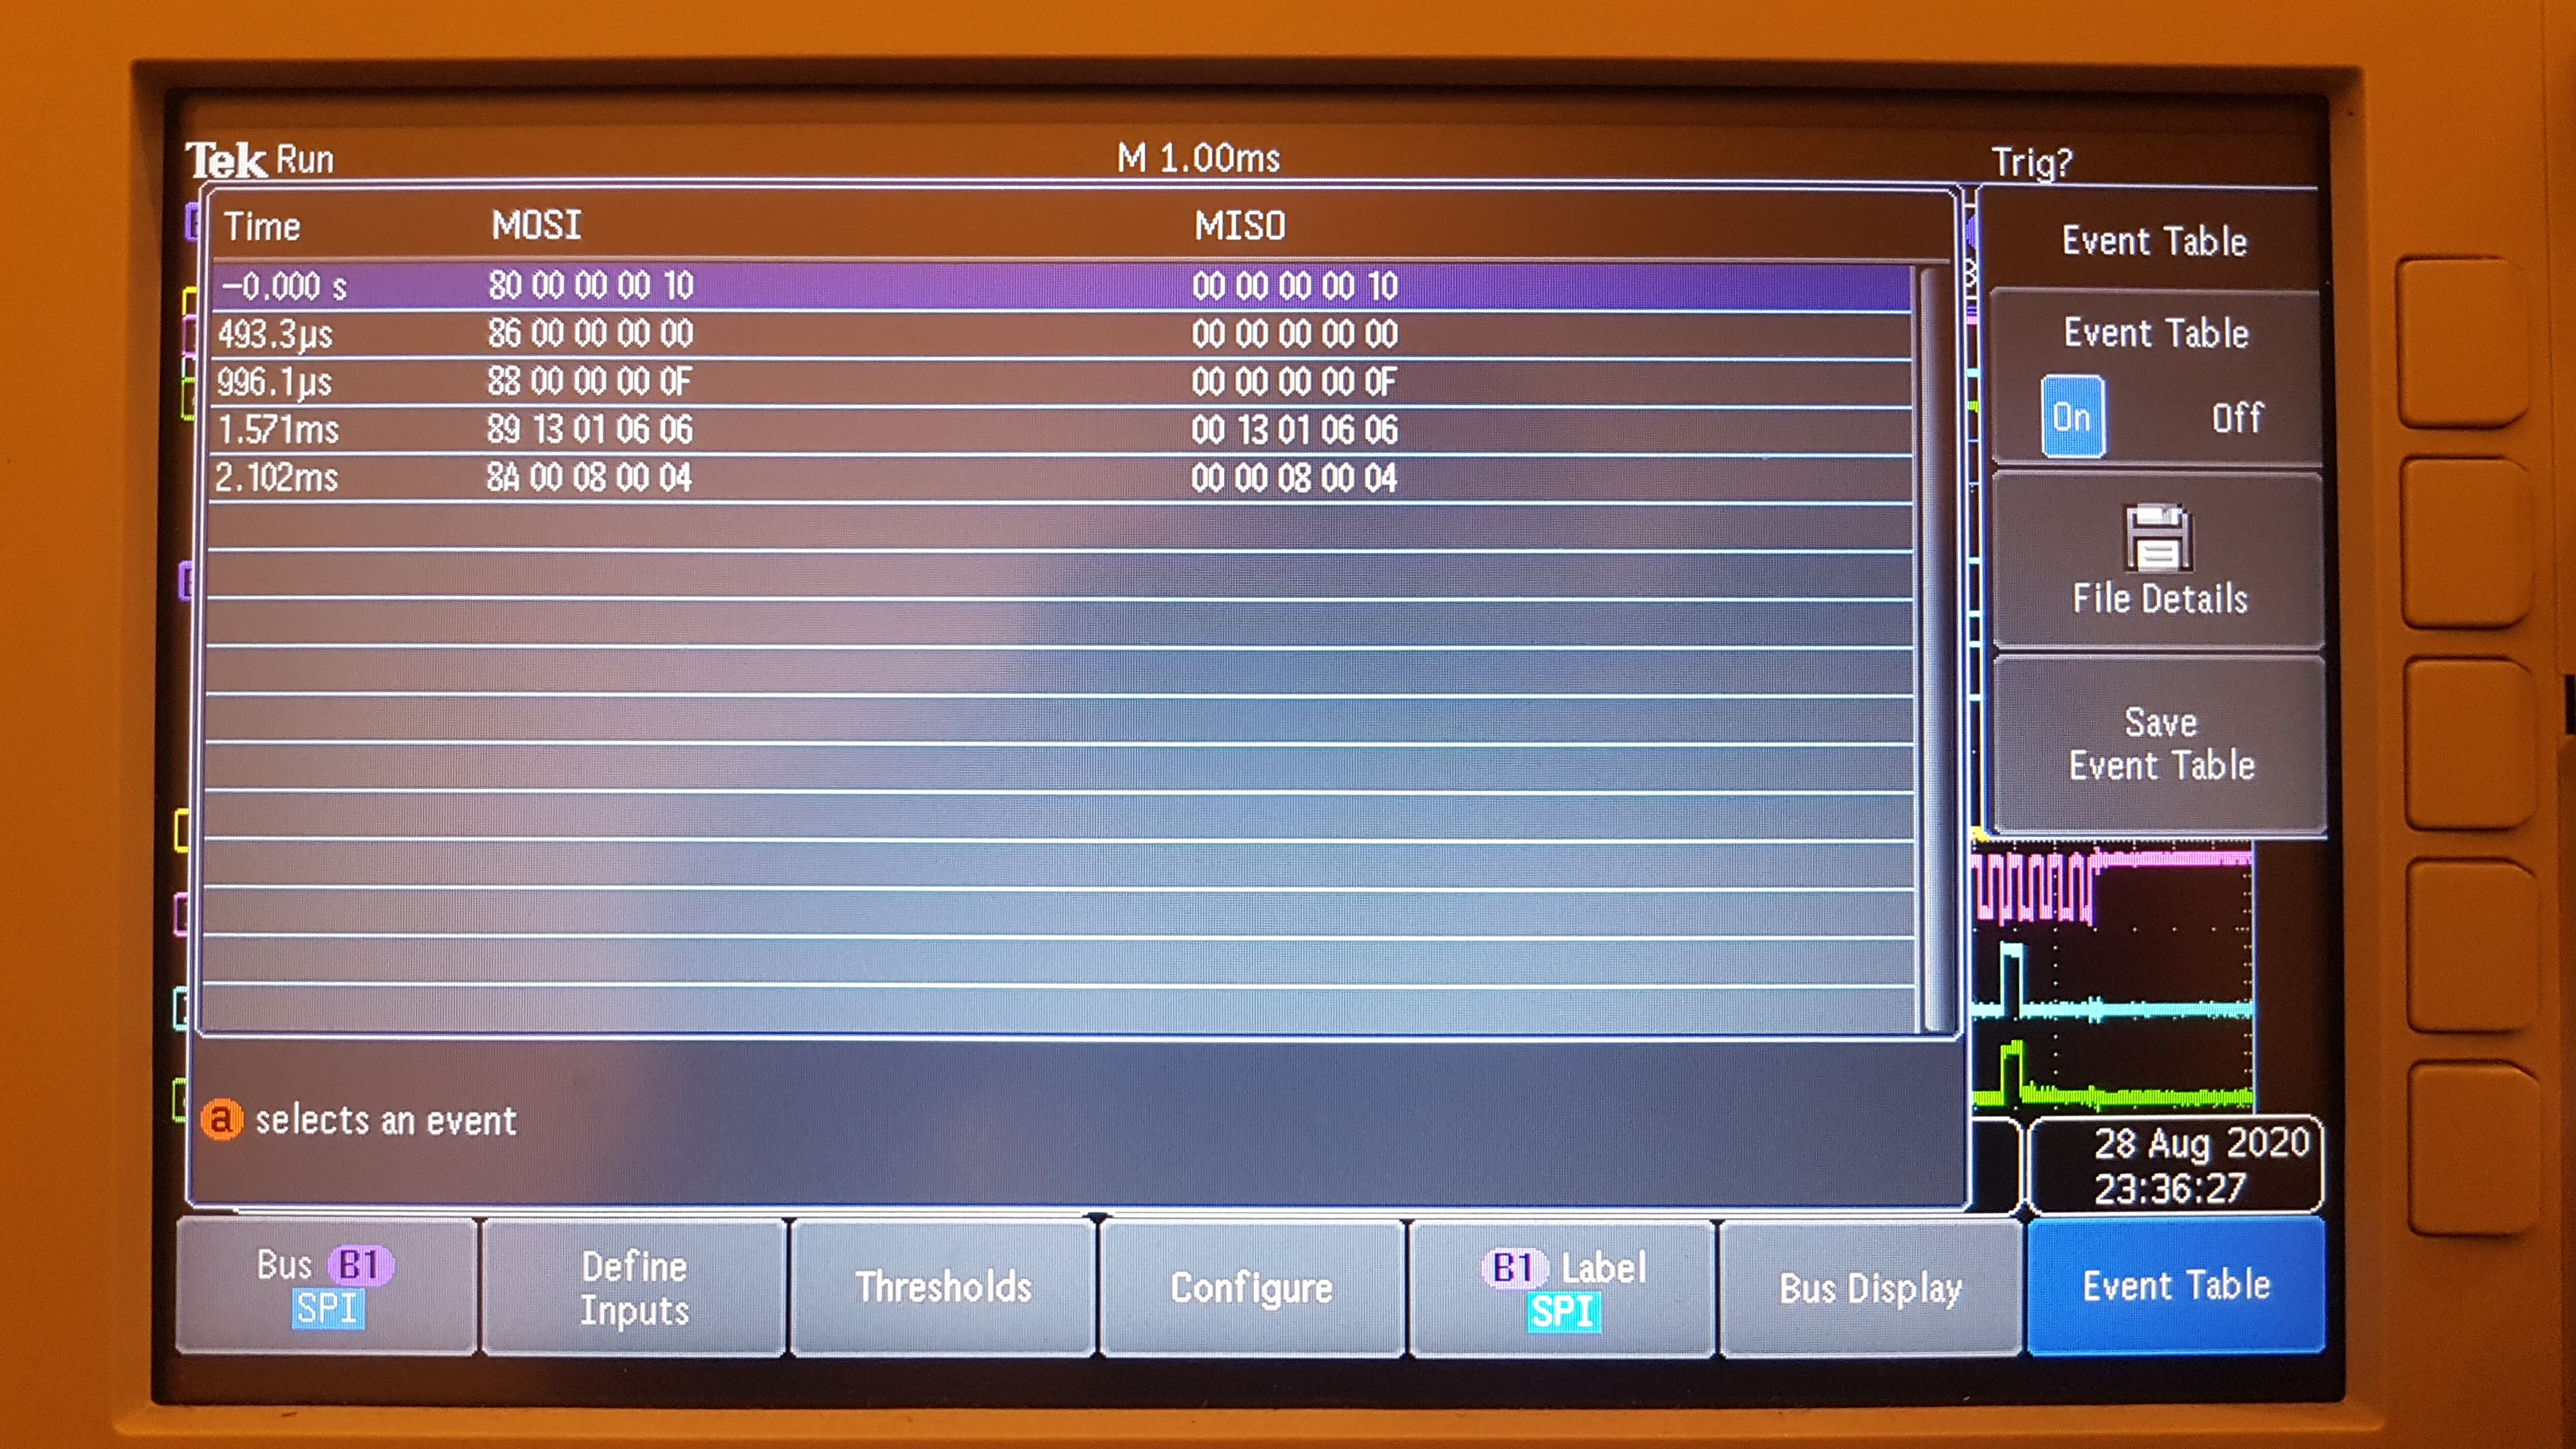
\includegraphics[width = \textwidth]{graphics/TMC6200_EventTable_Beschreiben_Bild}
\caption{Event-Table Inbetriebnahme TMC6200.}
\label{fig:TMC6200_EventTable_Beschreiben_Bild}
\end{figure}

\begin{figure}[h!]
\center
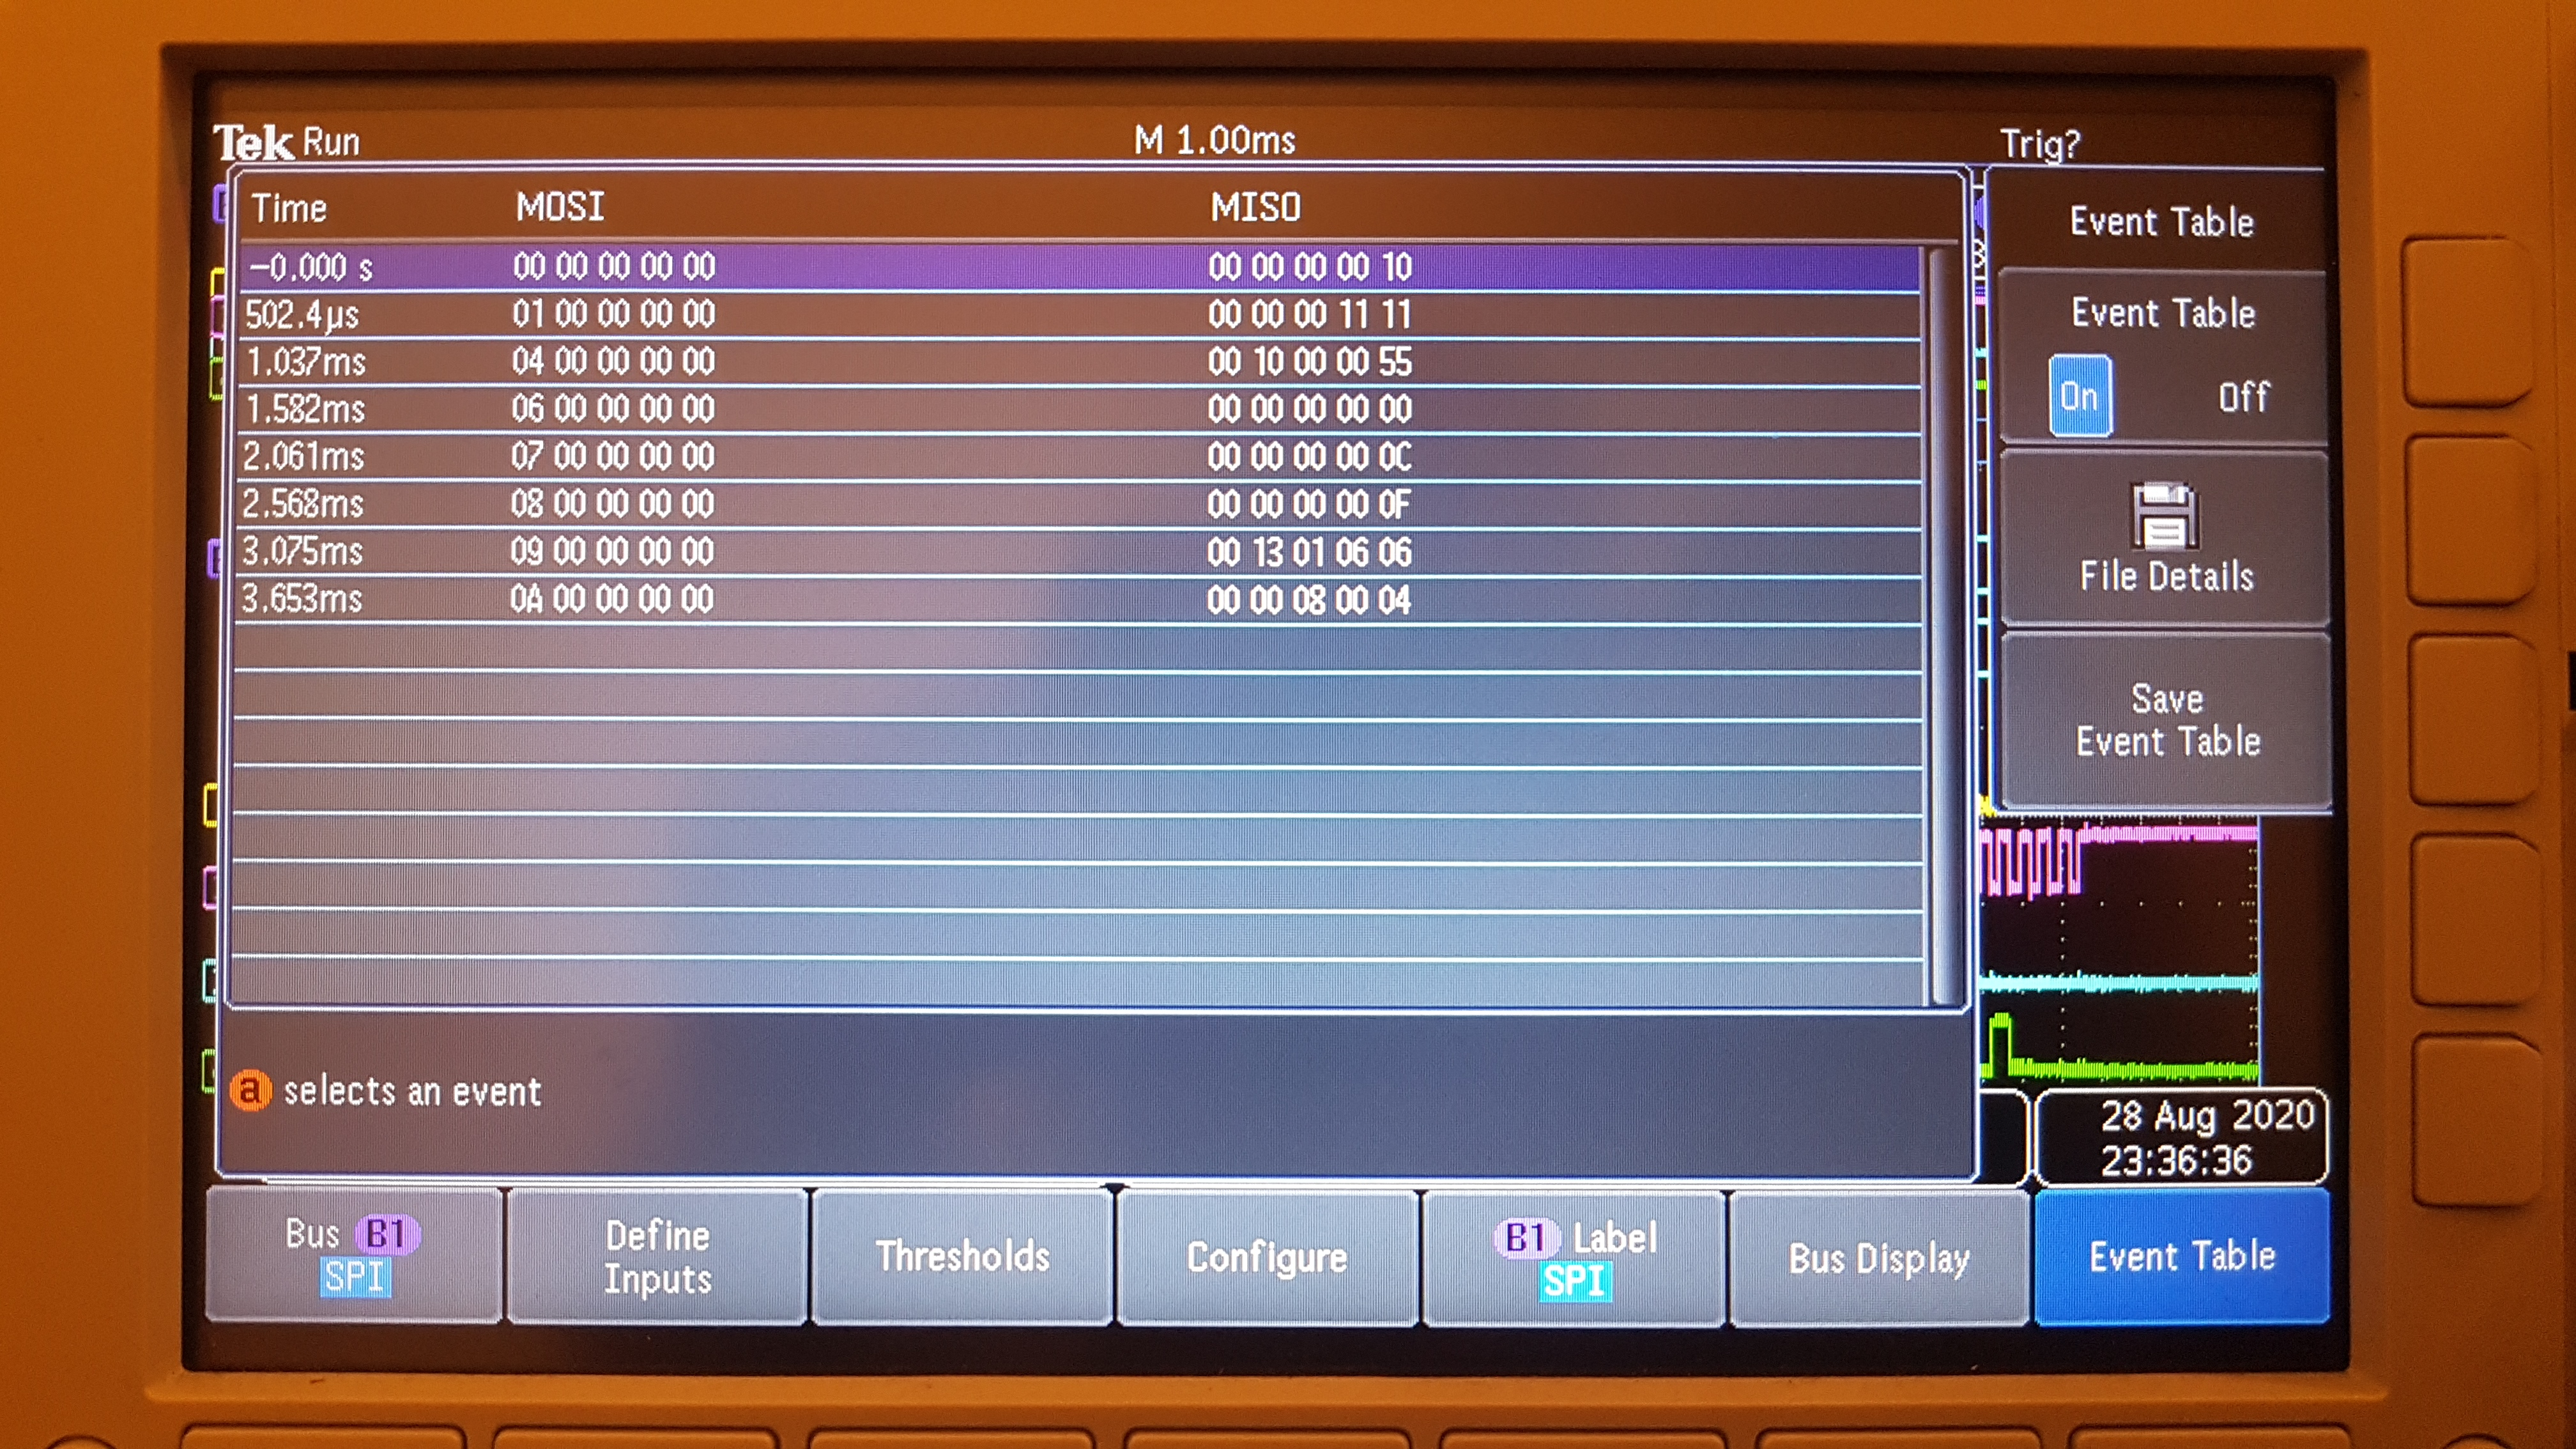
\includegraphics[width = \textwidth]{graphics/TMC6200_EventTable_Lesen_Bild}
\caption{Event-Table Inbetriebnahme TMC6200.}
\label{fig:TMC6200_EventTable_Lesen_Bild}
\end{figure}

\newpage

\subsubsection{Inbetriebnahme Gate-Ctrl}\label{Appendix:TMC6200_Gate_Ctrl}

\begin{figure}[h!]
\center
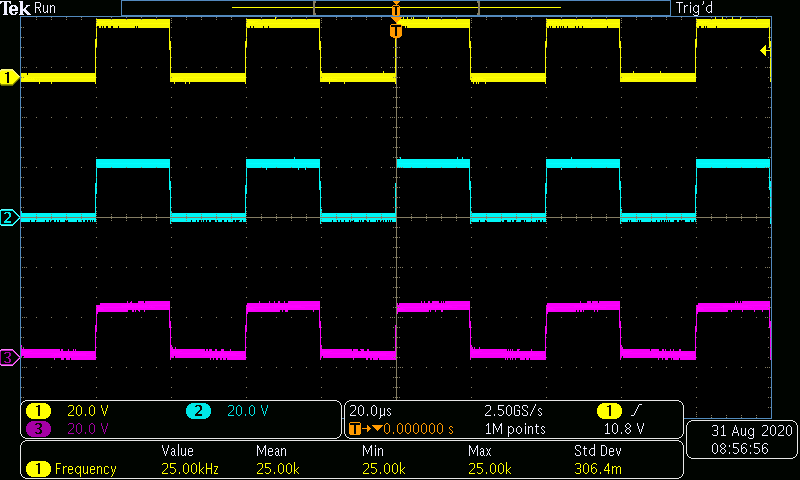
\includegraphics[width = \textwidth]{graphics/TMC6200_Gate_Signal_H}
\caption{Steuersignale PWM 48V von TMC6200 auf H-Brücke. Gelb = U, Blau = V, Magenta = W}
\label{fig:TMC6200_Gate_Signal_H}
\end{figure}

\begin{figure}[h!]
\center
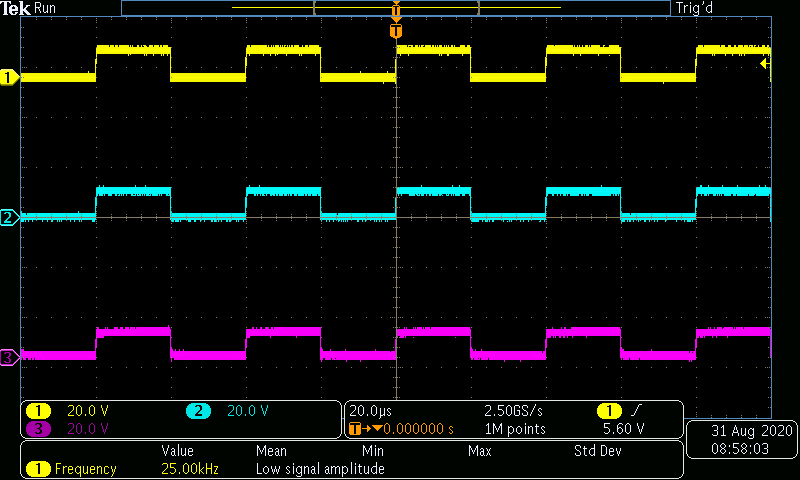
\includegraphics[width = \textwidth]{graphics/TMC6200_Gate_Signal_L}
\caption{Steuersignale PWM 0V von TMC6200 auf H-Brücke. Gelb = U, Blau = V, Magenta = W}
\label{fig:TMC6200_Gate_Signal_L}
\end{figure}

\newpage

\section{H-Brücke}\label{Appendix:H_Bruecke}

\subsection{Referenzschema}

\begin{figure}[h!]
	\centering
	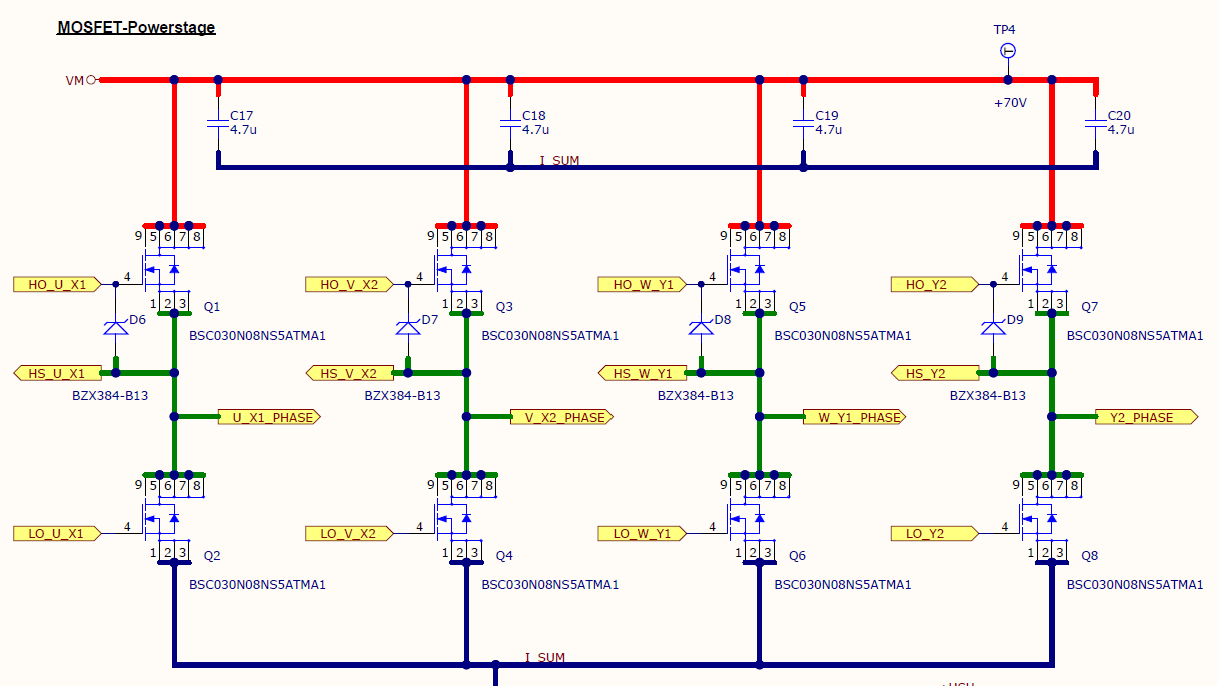
\includegraphics[width=0.9\textwidth]{graphics/Referenzschema_10A70V}
	\caption{H-Brücke.}
	\label{fig:Schema_H_Bruecke_und_BLDC_Ref}
\end{figure}

%\todo{cite: Datenblatt UPS 10A70V Schema}

\subsection{Inbetriebnahme}

\subsubsection{Inbetriebnahme Setup}\label{Appendix:H_Bruecke_Setup}

\begin{figure}[h!]
	\centering
	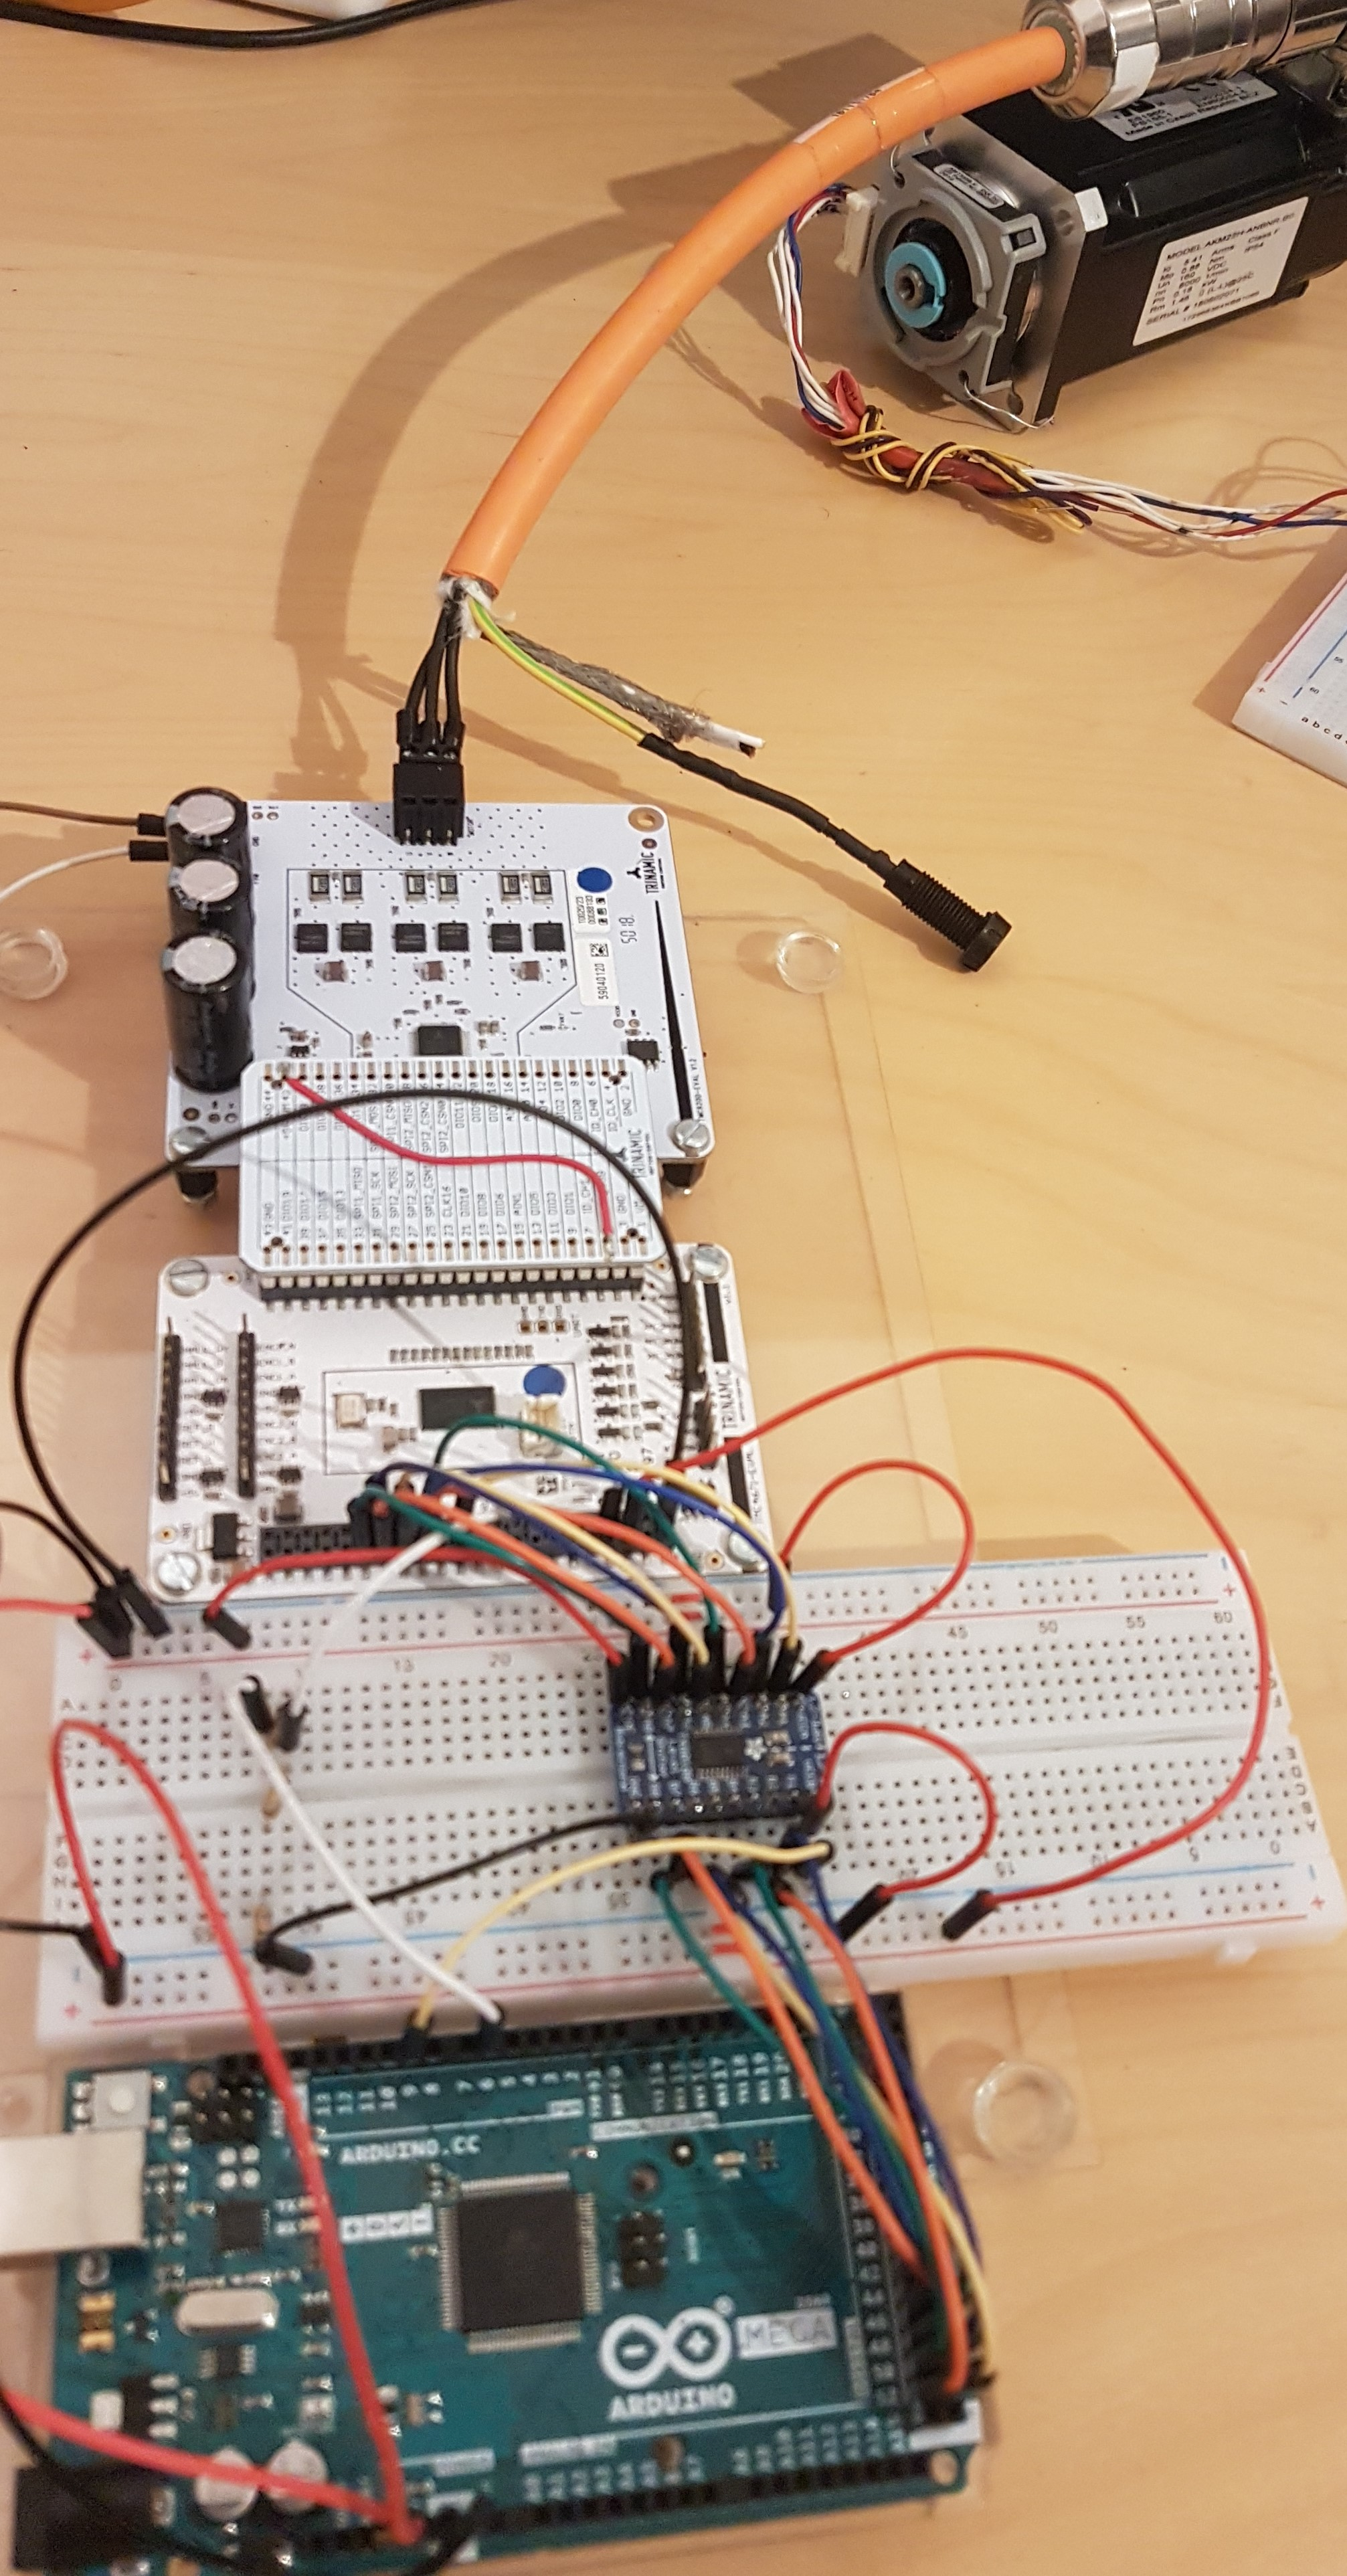
\includegraphics[angle =270, width=0.9\textwidth]{graphics/3_normal}
	\caption{Setup Inbetriebnahme H-Brücke und Motor.}
	\label{fig:3_normal}
\end{figure}

\newpage

\subsubsection{Inbetriebnahme Schaltsignale}\label{Appendix:H_Bruecke_Schaltsignale}

\begin{figure}[h!]
	\centering
	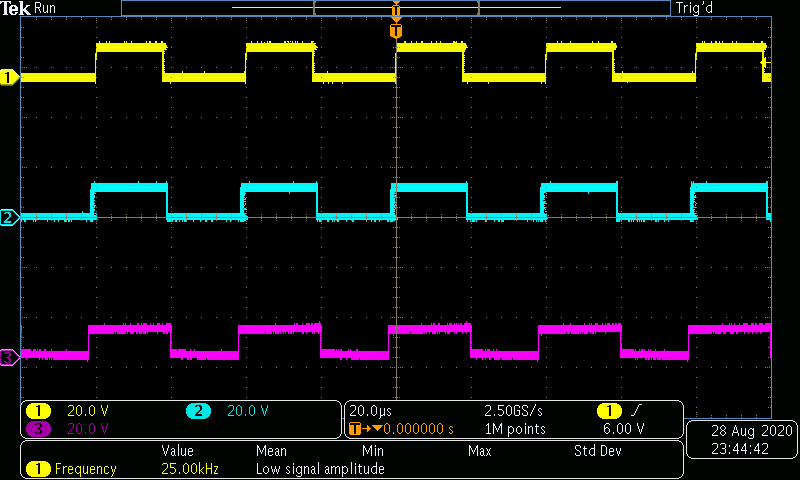
\includegraphics[width=\textwidth]{graphics/OpenLoop_TestDrive2}
	\caption{Schaltsignale während dem Openloop Testdrive. Gelb = U, Blau = V, Magenta = W}
	\label{fig:OpenLoop_TestDrive2}
\end{figure}

\newpage

\section{CUI AMT332S-V ABN-Encoder}\label{Appendix:ABC_Ecoder}

\subsection{Pinout and Interface}

\begin{figure}[h!]
	\centering
	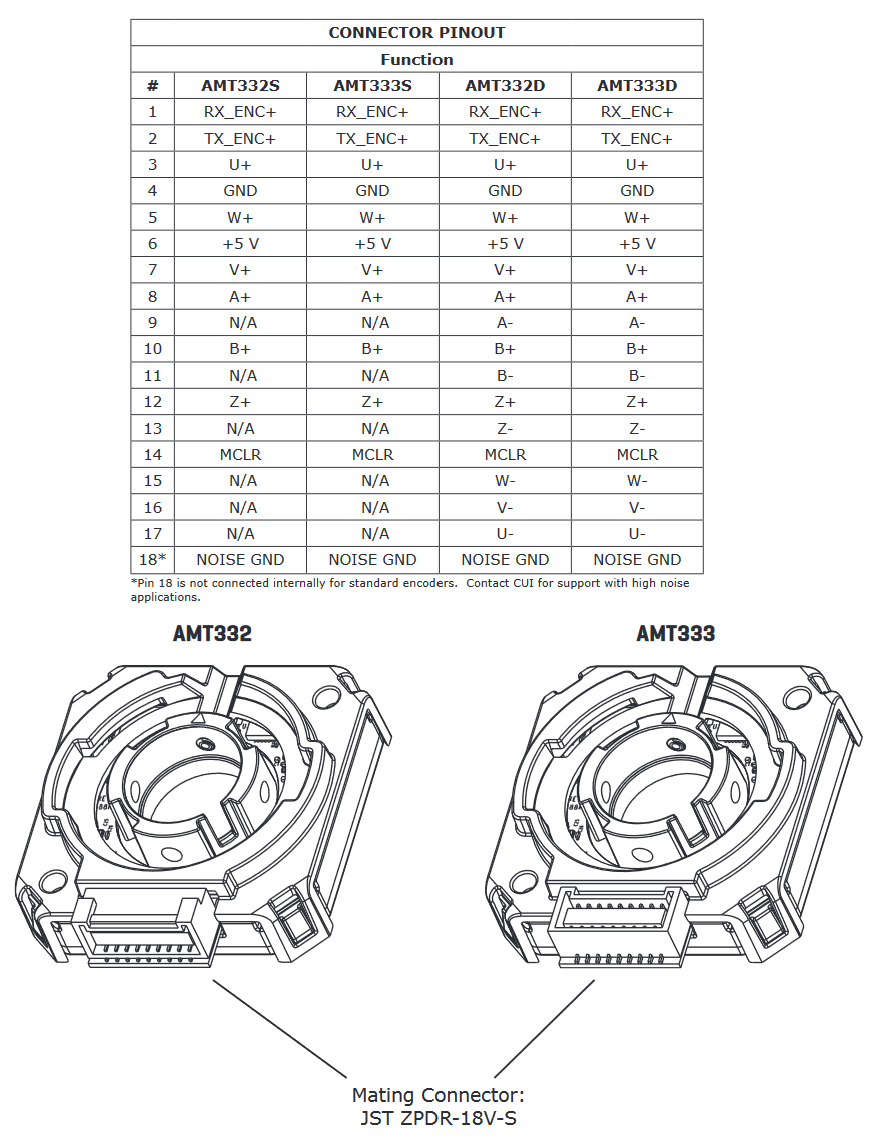
\includegraphics[width=\textwidth]{graphics/Encoder_Interface}
	\caption{Encoder-Interface Pinout-Table.}
	\label{fig:Encoder_Interface}
\end{figure}

\newpage

\subsection{Inbetriebnahme}

\subsubsection{Inbetriebnahme Setup}\label{Appendix:ABN_Setup}

\begin{figure}[h!]
	\centering
	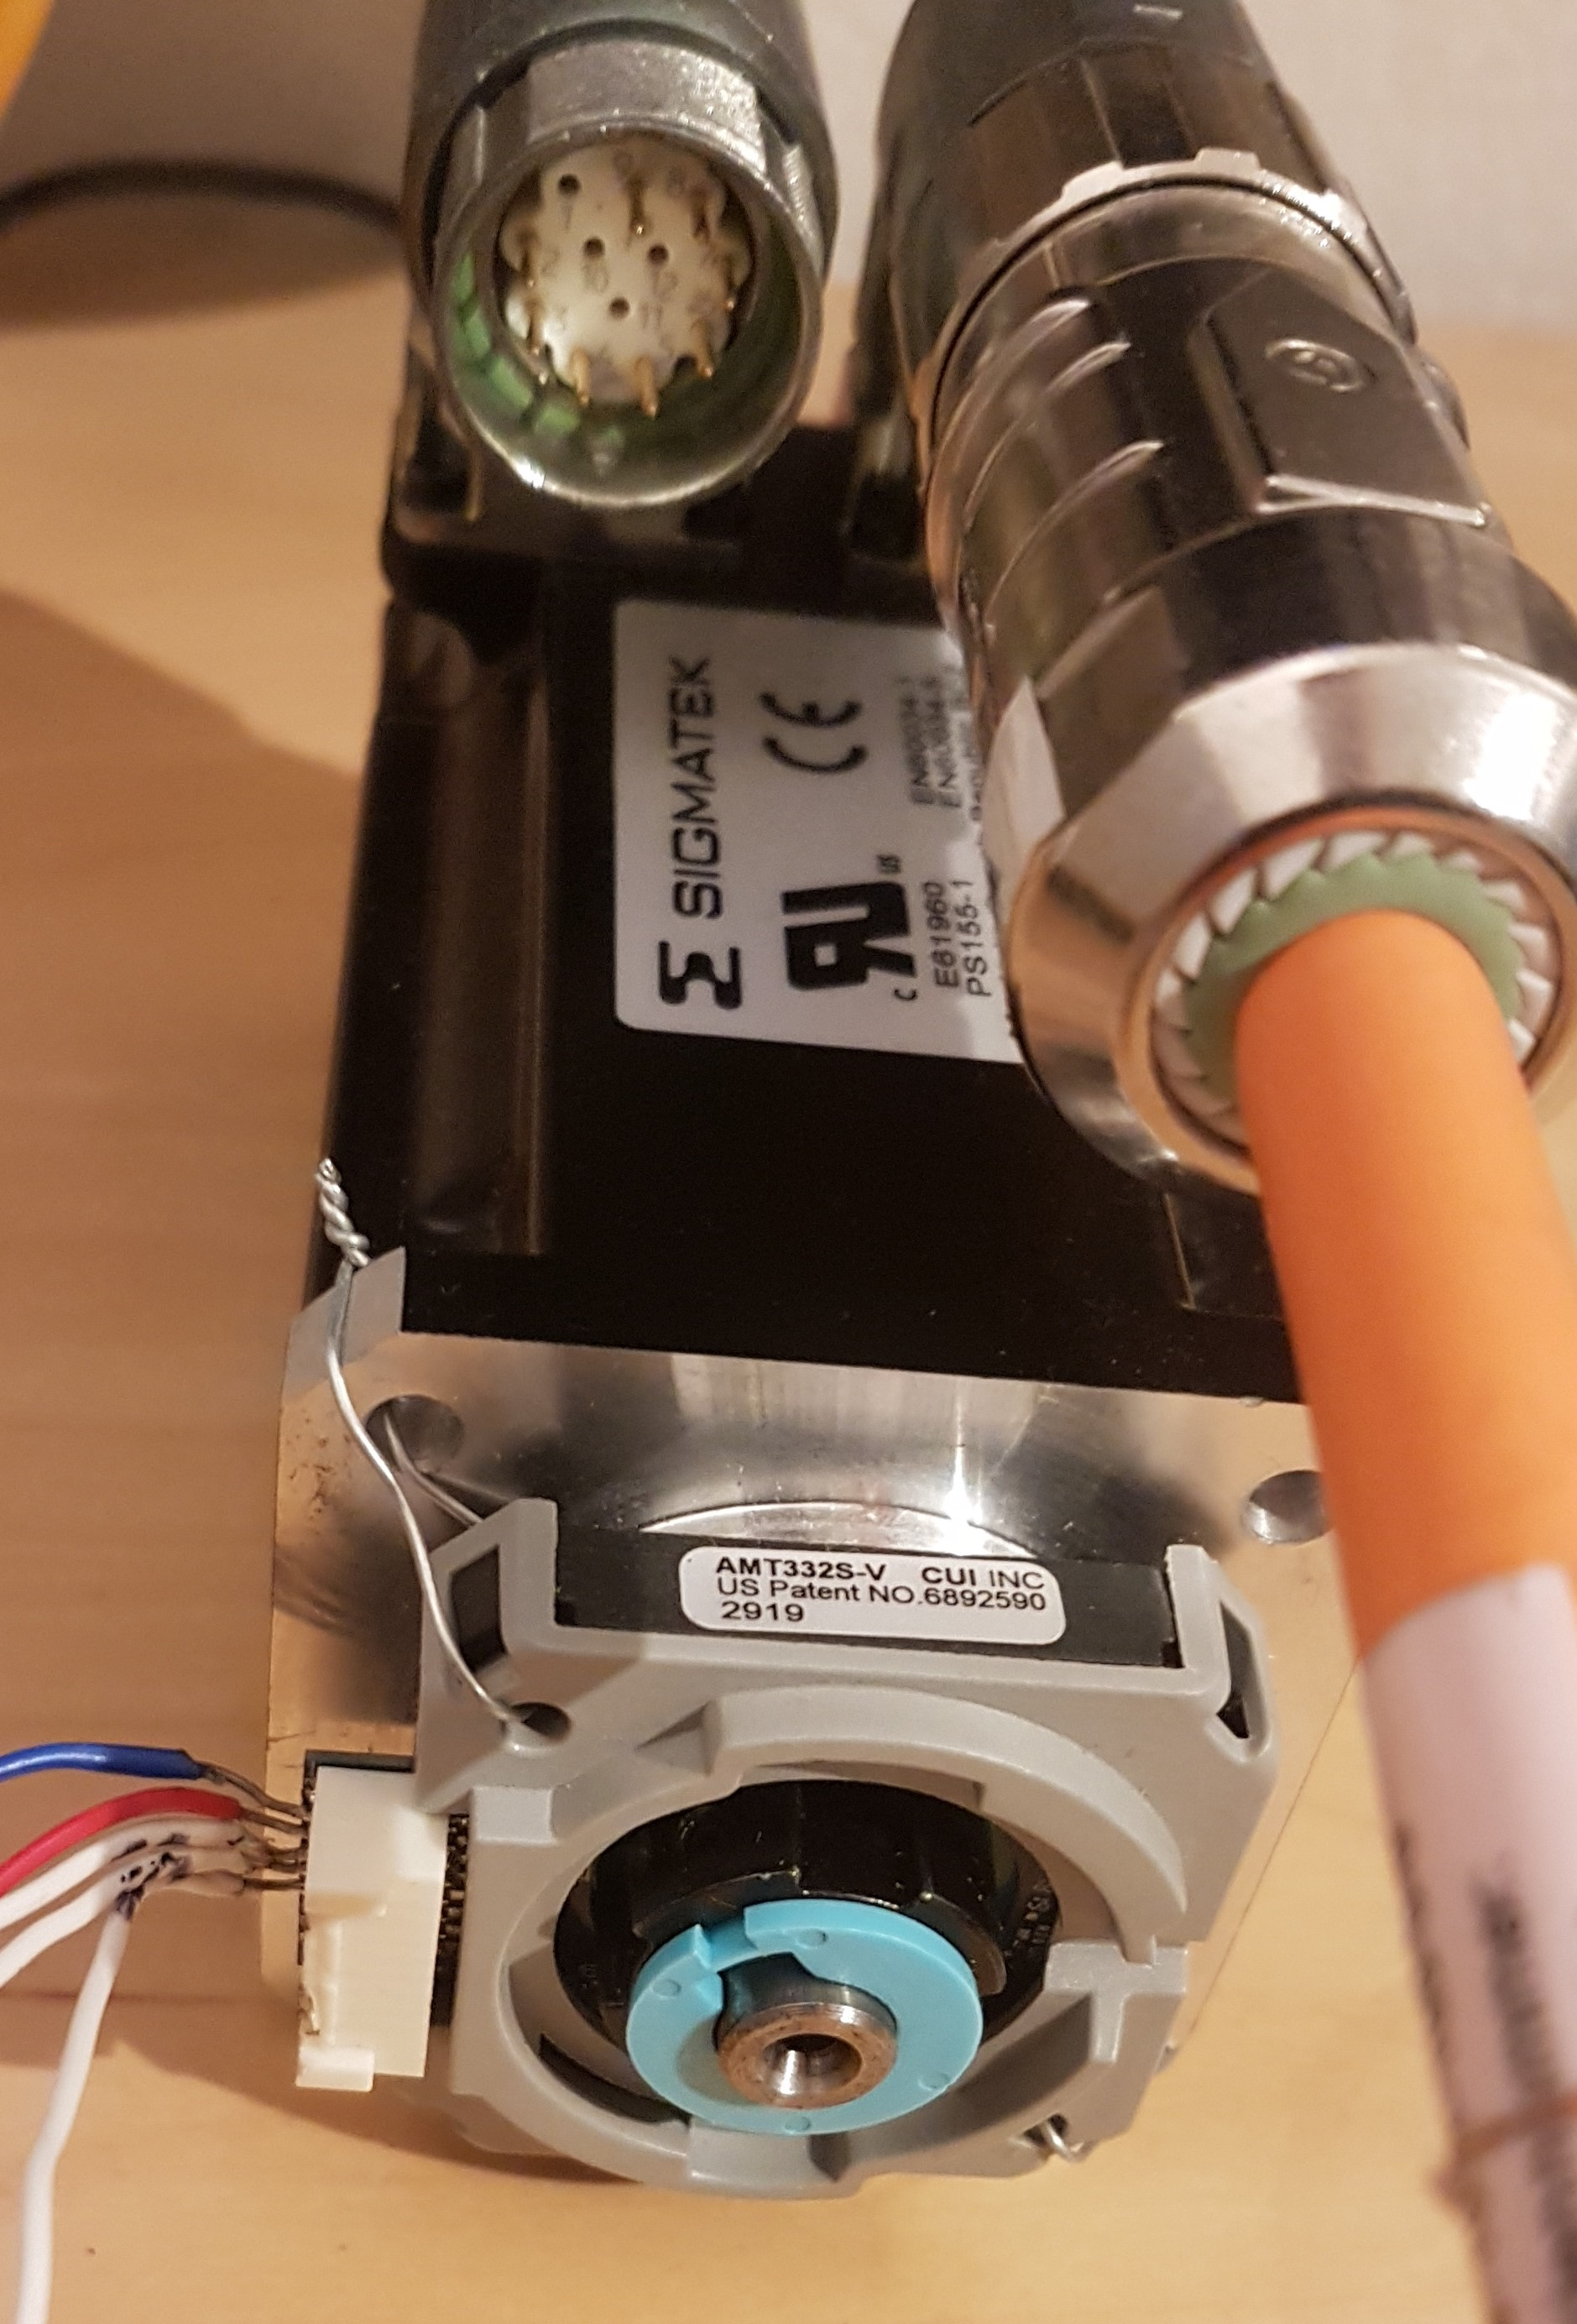
\includegraphics[angle = 270, width=\textwidth]{graphics/4_Encoder_Motor}
	\caption{Encoder-Interface Pinout-Table.}
	\label{fig:4_Encoder_Motor}
\end{figure}

\begin{figure}[h!]
	\centering
	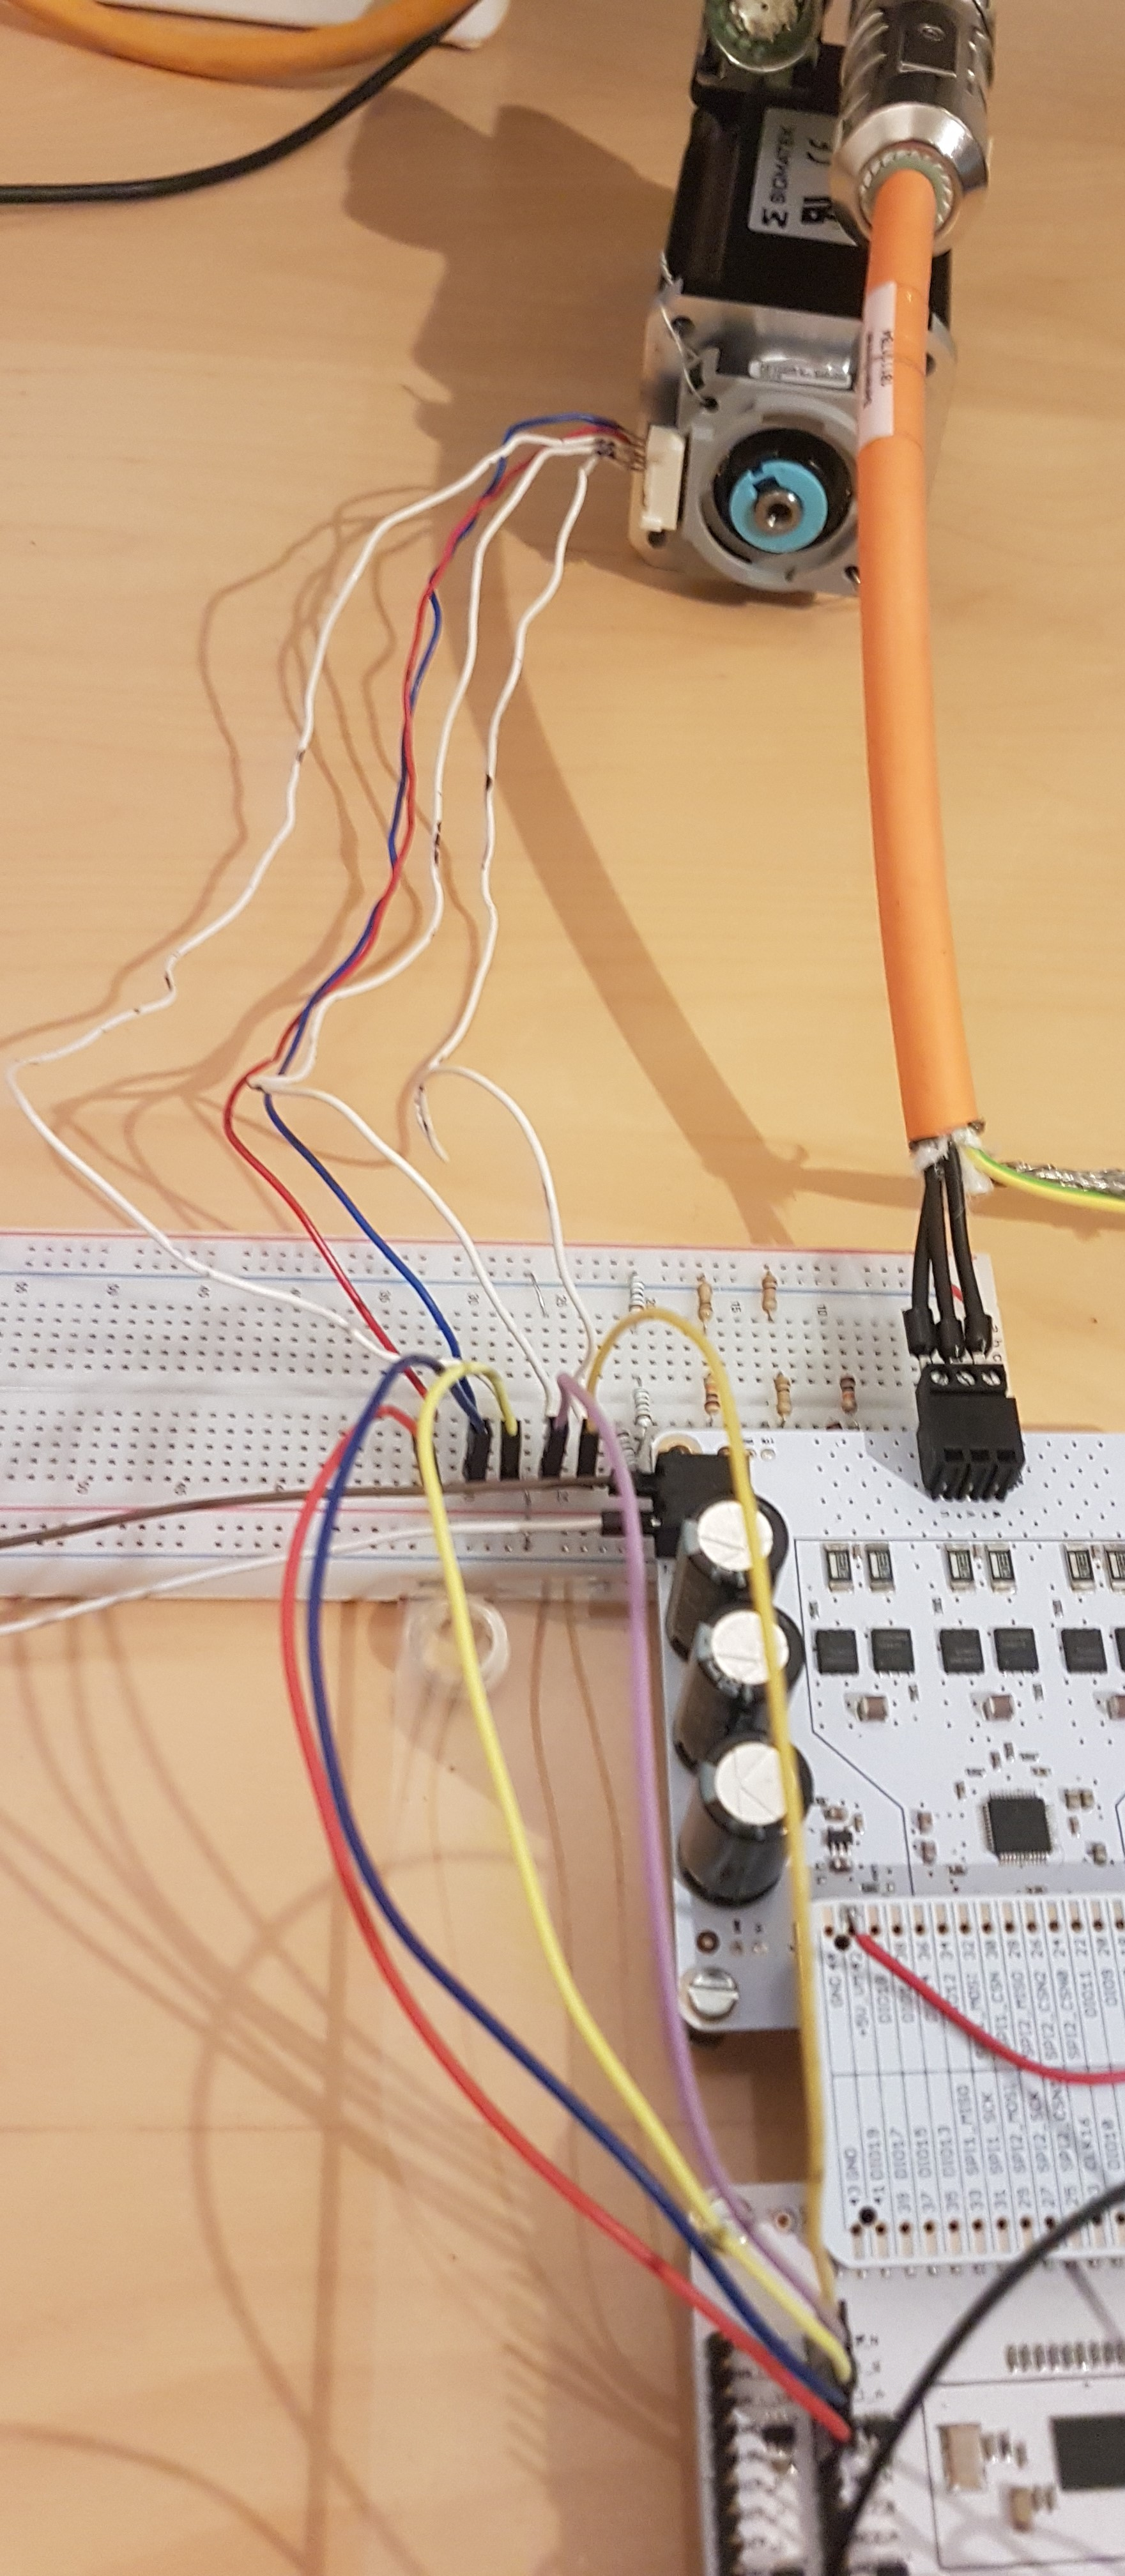
\includegraphics[angle = 270, width=\textwidth]{graphics/4_Antriebskette}
	\caption{Encoder-Interface Pinout-Table.}
	\label{fig:4_Antriebskette}
\end{figure}

\newpage

\begin{figure}[h!]
	\centering
	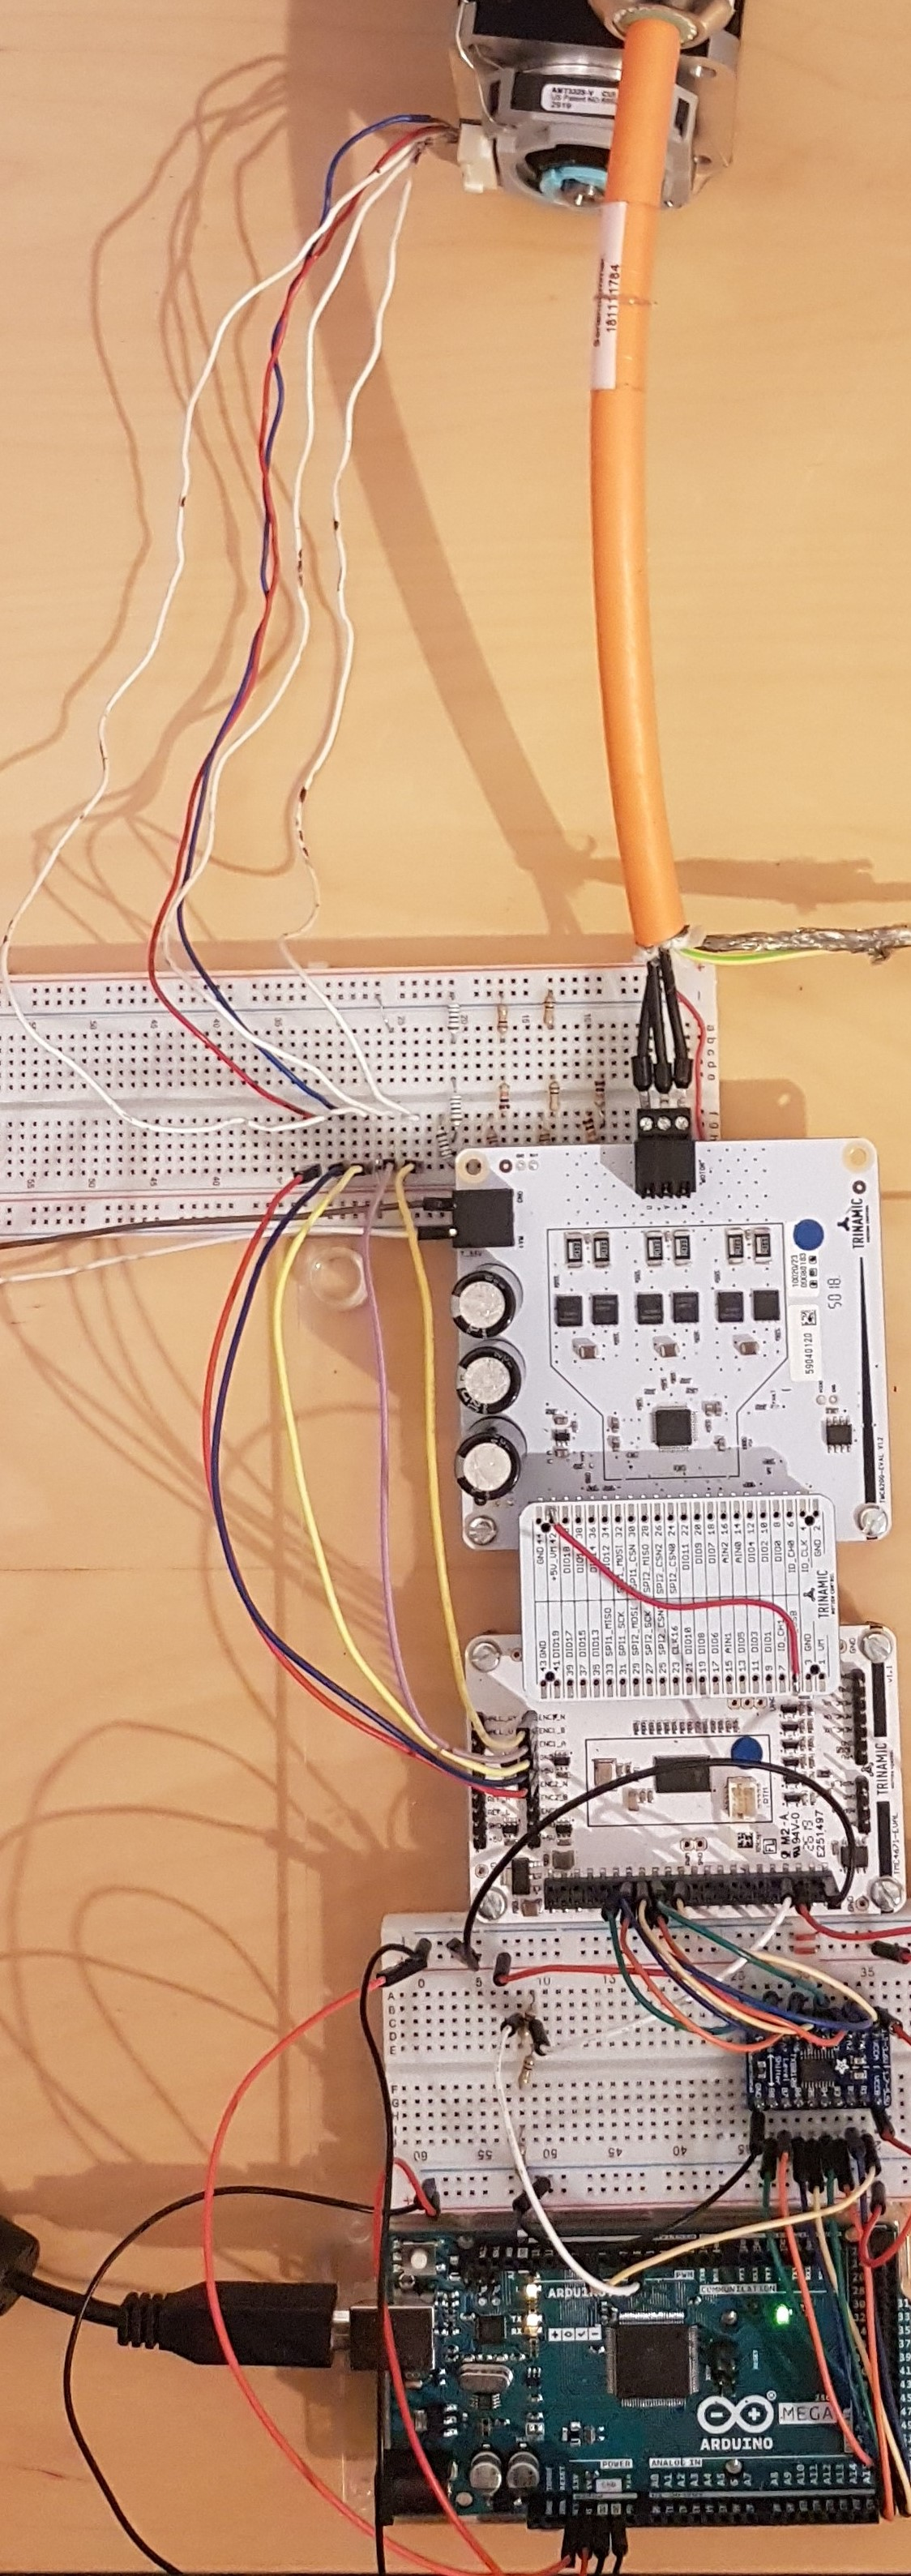
\includegraphics[angle = 270, width=\textwidth]{graphics/4_komplett}
	\caption{Encoder-Interface Pinout-Table.}
	\label{fig:4_komplett}
\end{figure}

\begin{figure}[h!]
	\centering
	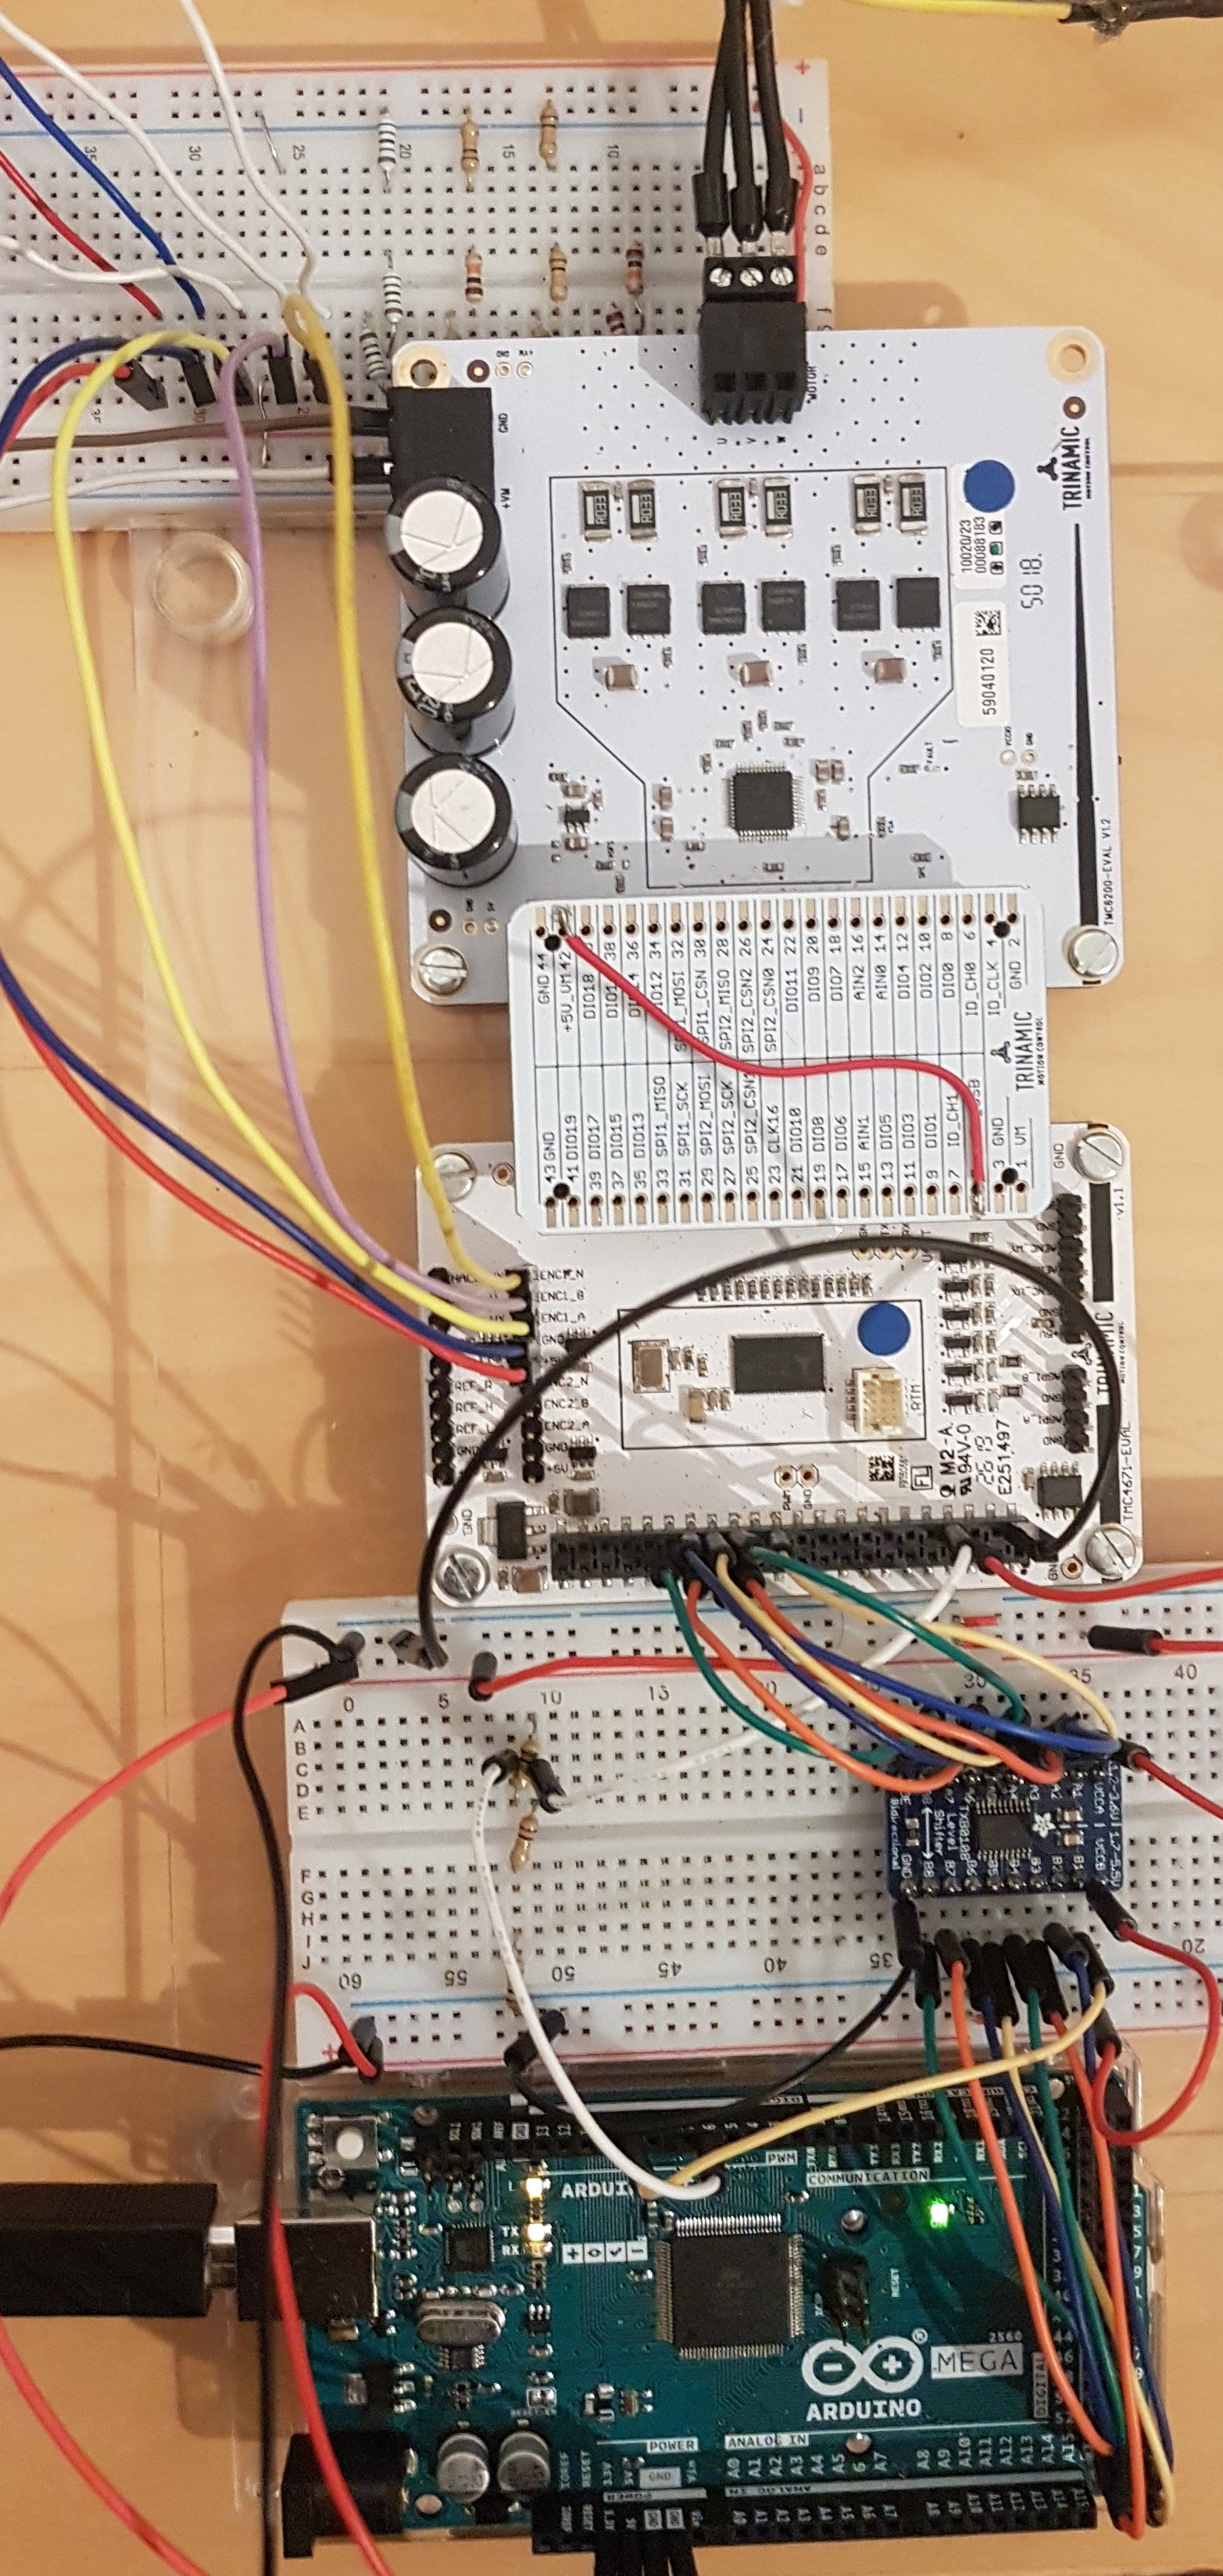
\includegraphics[angle = 270, width=\textwidth]{graphics/4_Elektronik}
	\caption{Encoder-Interface Pinout-Table.}
	\label{fig:4_Elektronik}
\end{figure}

\newpage

\subsubsection{Encoder-Signale}\label{Appendix:ABN_Signale}

\begin{figure}[h!]
	\centering
	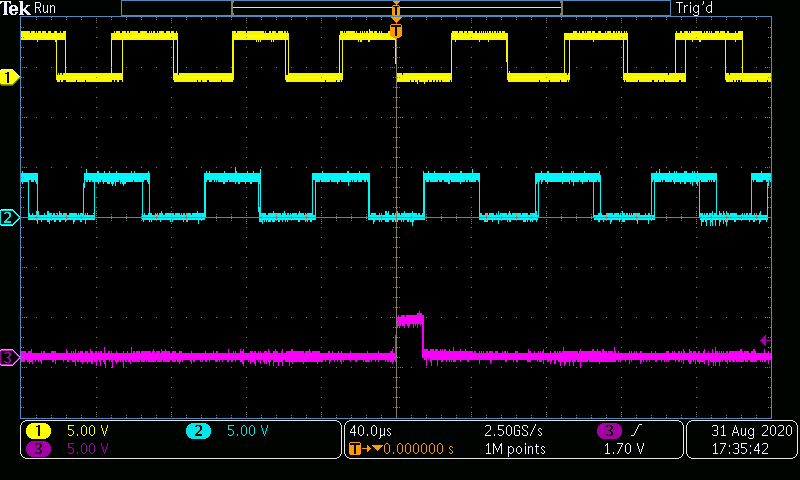
\includegraphics[width=\textwidth]{graphics/AMT322S-V_Signal}
	\caption{Encoder-Interface Pinout-Table. Gelb = A, Blau = B, N = Magenta}
	\label{fig:AMT322S-V_Signal}
\end{figure}

\newpage

\section{Mikrocontroller}\label{Appendix:Mikrocontroller}

\subsection{Brown-out-Detection}\label{Appendix:Brown-out-Detection}

\begin{figure}[h!]
	\centering
	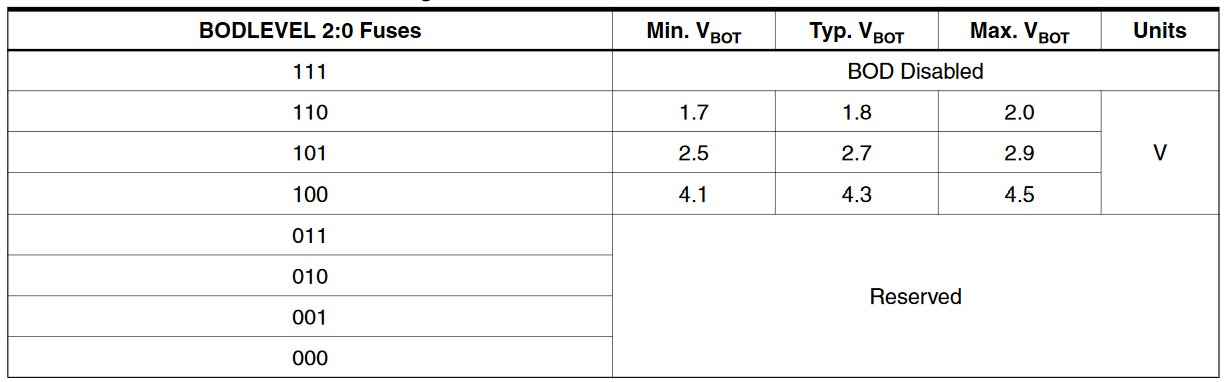
\includegraphics[width=0.7\textwidth]{graphics/Tabelle_BoD}
	\caption{Tabelle Brown-out-Detection.}
	\label{fig:Tabelle_BoD}
\end{figure}

\todo{cite: Datenblatt Atmega 2560, Seite 361}

\subsection{Full Swing Crystal Oscillator}\label{Appendix:Full_Swing _Crystal_Oscillator}

\begin{figure}[h!]
	\centering
	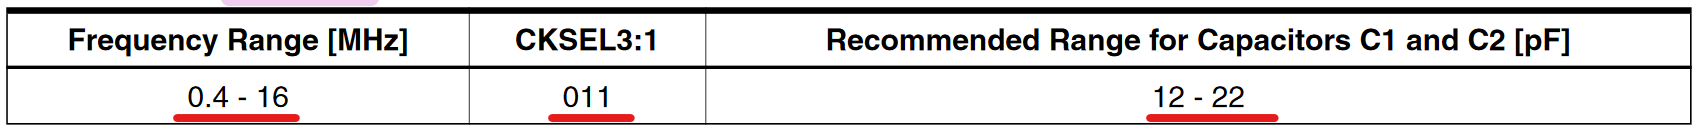
\includegraphics[width=0.7\textwidth]{graphics/Tabelle_Crystal}
	\caption{Tabelle Frequenzbereich Crystal Oszillator.}
	\label{fig:Tabelle_Crystal}
\end{figure}

\todo{cite: Datenblatt Atmega 2560, Seite 43}

\begin{figure}[h!]
	\centering
	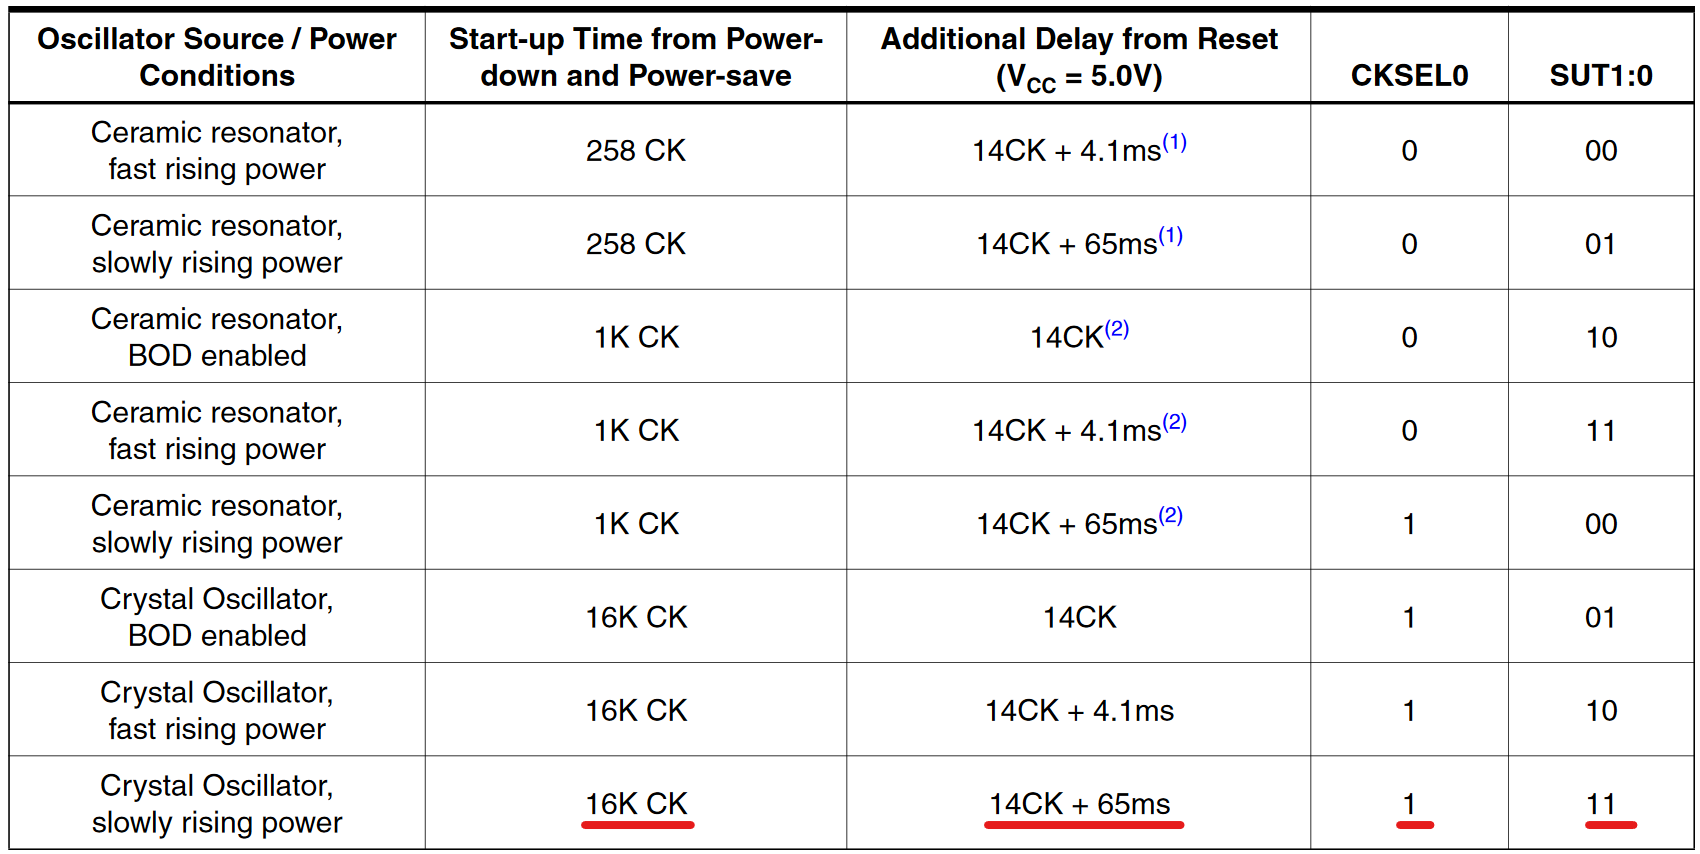
\includegraphics[width=0.7\textwidth]{graphics/Tabelle_Crystal2}
	\caption{Tabelle Aufstartzeit.}
	\label{fig:Tabelle_Crystal2}
\end{figure}

\todo{cite: Datenblatt Atmega 2560, Seite 43}

\subsection{Bootloader-Speicherplatz}\label{Appendix:Bootloader-Speicherplatz}

\begin{figure}[h!]
	\centering
	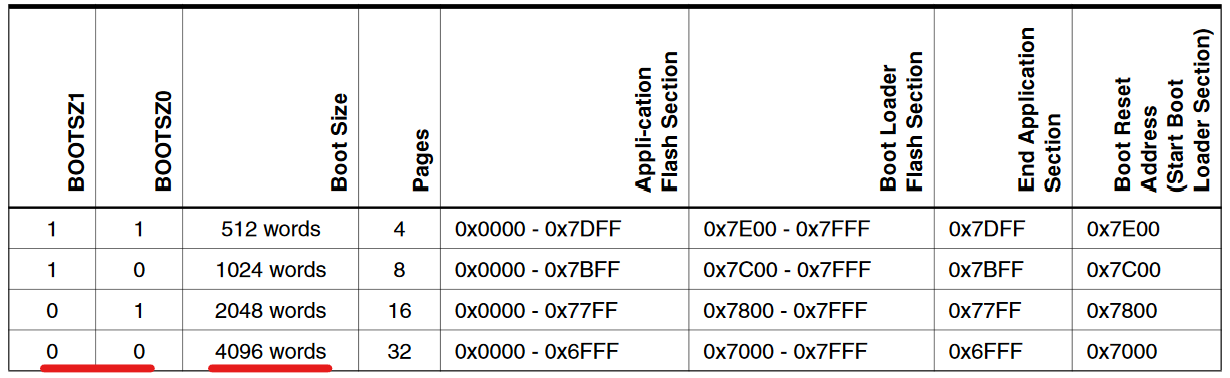
\includegraphics[width=0.7\textwidth]{graphics/Tabelle_Bootloader}
	\caption{Tabelle Bootloader Speicherplatz.}
	\label{fig:Tabelle_Bootloader}
\end{figure}

\todo{cite: Datenblatt Atmega 2560, Seite 320}

\subsection{Memory-Lock Bootloader}

\begin{figure}[h!]
	\centering
	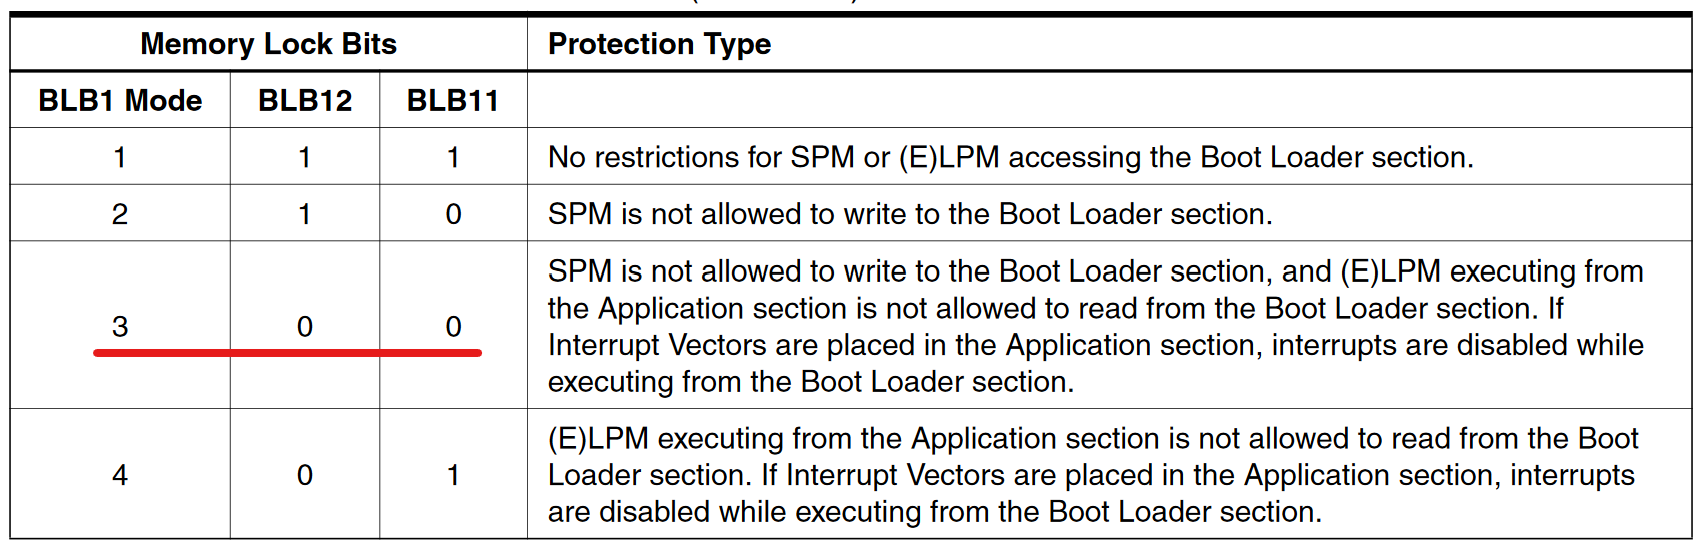
\includegraphics[width=0.7\textwidth]{graphics/Tabelle_Memory_Lock}
	\caption{Tabelle Memory Lock.}
	\label{fig:Tabelle_Memory_Lock}
\end{figure}

\todo{cite: Datenblatt Atmega 2560, Seite 326}

\newpage
\section{USB-B}\label{Appendix:USB_B}

\subsection{Geräte-Manager}

\begin{figure}[h!]
\center
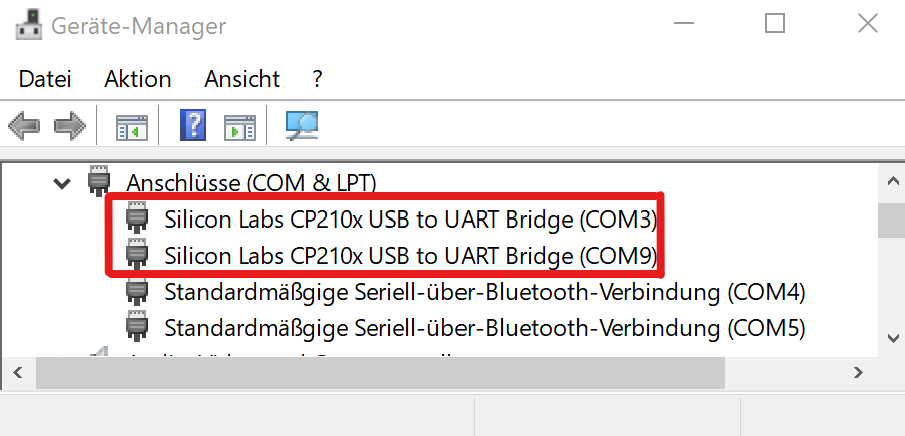
\includegraphics[width = 0.6 \textwidth]{graphics/USB_Devices_Ger_Man}
\caption{Geräte-Manager mit den aufgelisteten USB-UART-Converter (Mikrocontroller und WiFi-Modul).}
\label{fig:USB_Devices_Ger_Man}
\end{figure}

\section{Atmel Studio}\label{Appendix:Atmel_Studio}

\subsection{Fuse Bits}

\begin{figure}[h!]
	\centering
	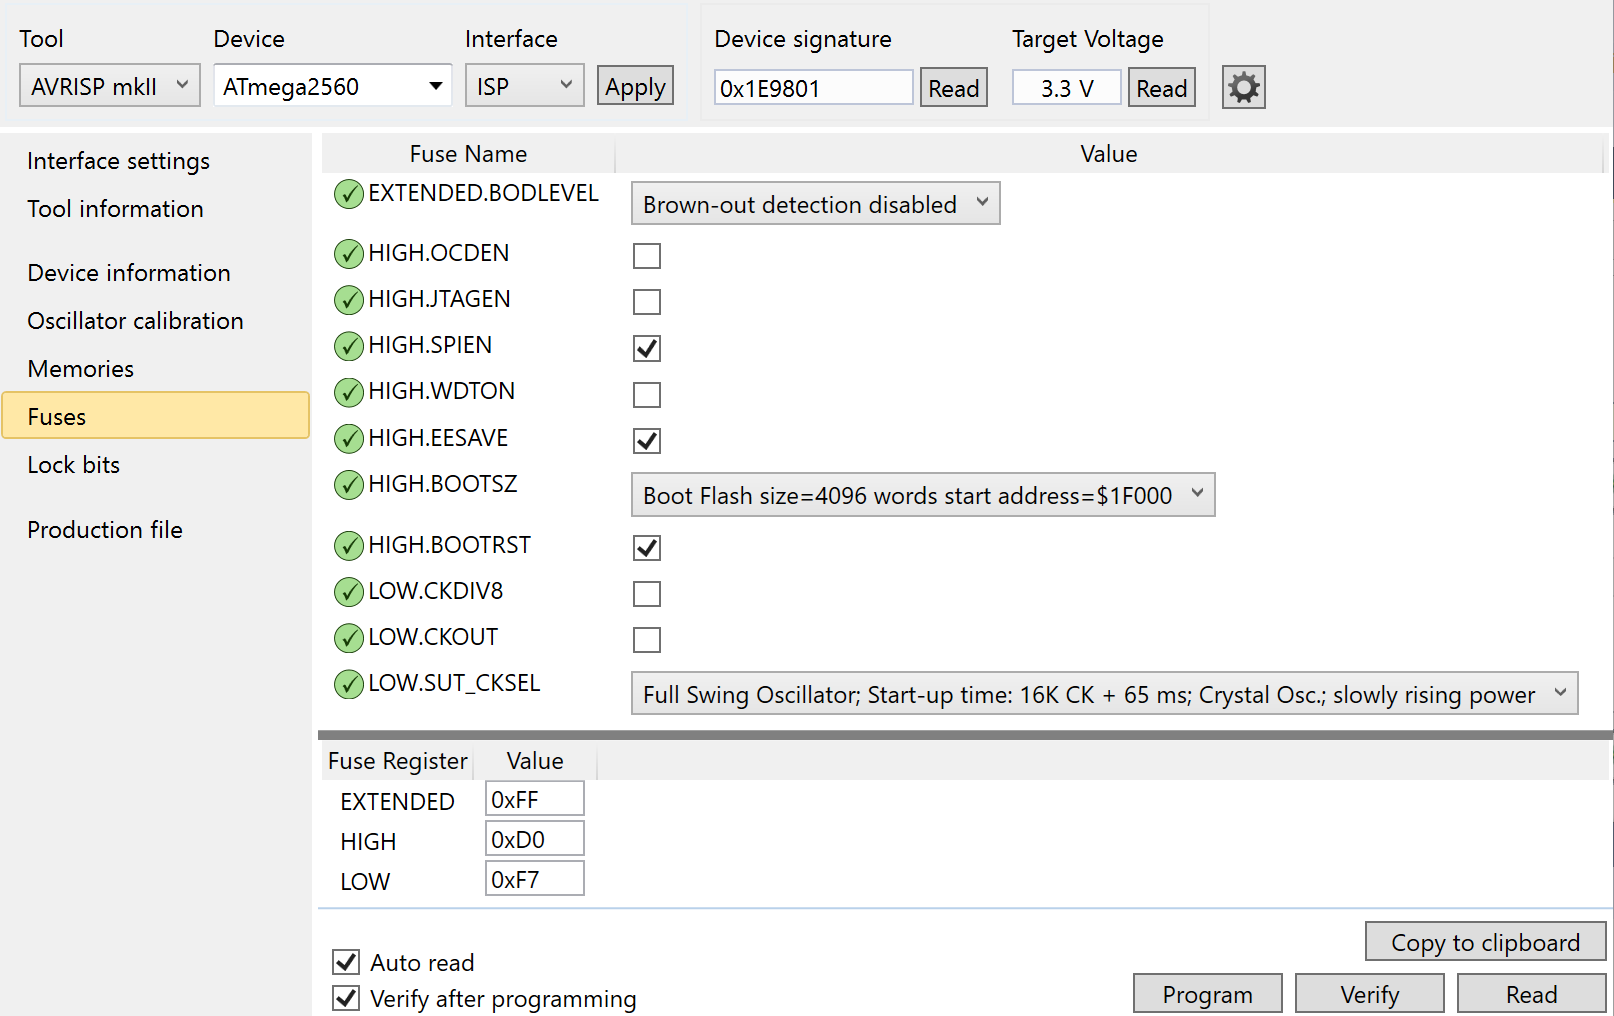
\includegraphics[width=\textwidth]{graphics/AtmelStudio_Fuses}
	\caption{Fuse-Bits Atmega2560.}
	\label{fig:AtmelStudio_Fuses}
\end{figure}

\subsection{Lock Bits}

\begin{figure}[h!]
	\centering
	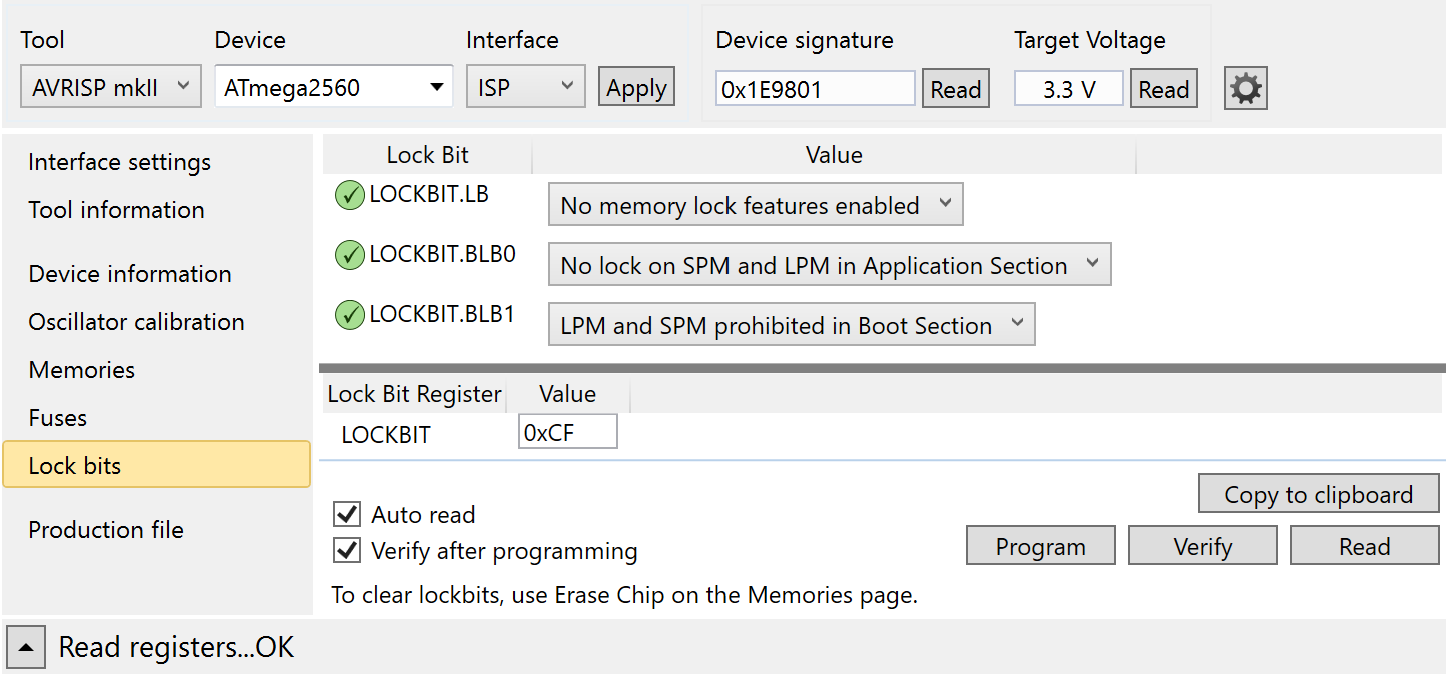
\includegraphics[width=\textwidth]{graphics/AtmelStudio_Locks}
	\caption{Lock-Bits Atmega2560.}
	\label{fig:AtmelStudio_Locks}
\end{figure}
\newpage
\subsection{Einbinden AVRdude und stk500v2 (wiring)}

\begin{figure}[h!]
	\centering
	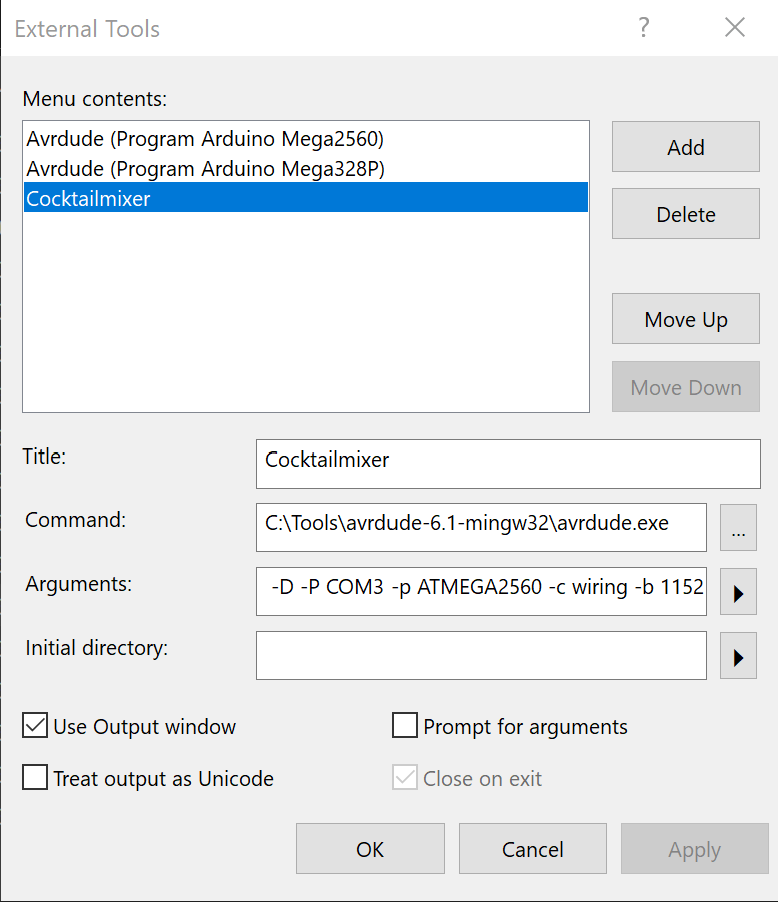
\includegraphics[width=0.5\textwidth]{graphics/AtmelStudio_External_Tools}
	\caption{External Tools Atmega2560.}
	\label{fig:AtmelStudio_Locks}
\end{figure}

\subsection{Bootloader ''Brennen''}

\begin{figure}[h!]
	\centering
	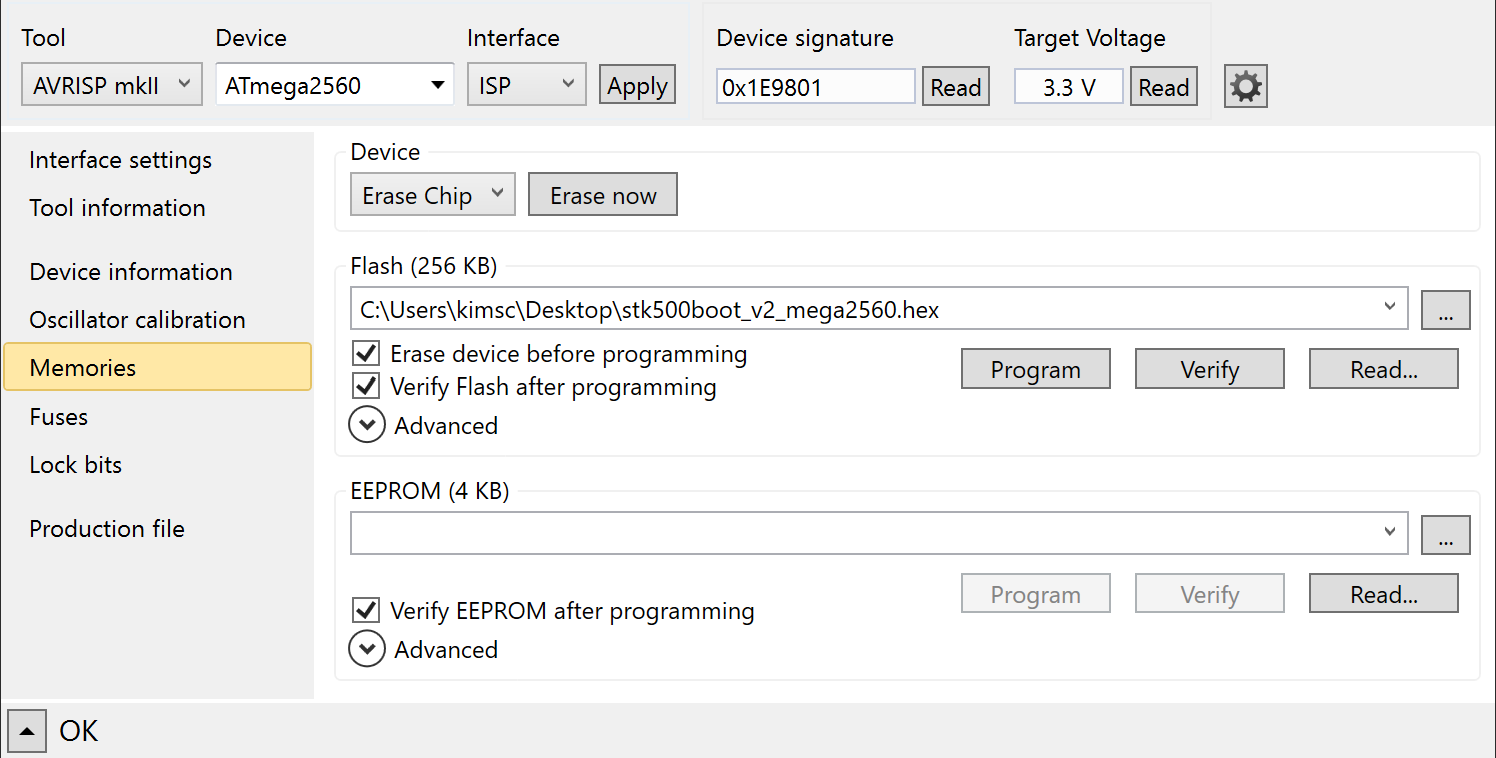
\includegraphics[width=\textwidth]{graphics/AtmelStudio_Program_Bootloader}
	\caption{Bootloader brennen.}
	\label{fig:AtmelStudio_Program_Bootloader}
\end{figure}

\end{appendix}